% ----------------------------------------------------------------
% Book Class (This is a LaTeX2e document)  ***********************
% ----------------------------------------------------------------
\documentclass[11pt,a4paper,onepage,openany]{book}
\usepackage[english]{babel}
\usepackage{graphicx}
\usepackage{epstopdf}

\def\<#1>{\texttt{<#1>}}
\def\[#1]{$[$#1$]$}

\author{Andreas Pott}
\title{WireX -- Scientific Software for Analysis and Design of Cable-driven
Parallel Robots\\[12em]
Confidential Report}
\date{last change: 23.06.2019, version 3.0.1022}
% ----------------------------------------------------------------
\begin{document}

\maketitle

\tableofcontents

\chapter{Preface and Objectives}\label{sec:Preface}%
The objective of this document is to describe and guide the development in the
WireX project. Most probably this documentation cannot be complete but giving
it a start is better than leaving everything open. This document describes
typical usage of WireCenter and gives an overview what can be done with the
program. When it comes to the second part i.e. the developer's guide, it is
tried to explain how things should be done and what was the rational behind
design decisions in the basic classes.

The documentation is a living document that can (and should) be extended and
completed by every developer of the WireX project.

\emph{WireCenter} is a simulation framework which is developed at Fraunhofer
IPA since 2009. It integrates different algorithms and tool chains
aiming at rapid development, design, simulation, investigation, calibration,
and control of cable-driven parallel robots. Its core features and algorithms
can be used with the integrated user interface, a MATLAB interface, or by a
dynamic link library which can be used in other software projects. The tool is
developed in C++ and uses OpenGL and MFC for visualization.

The development of the design Suite WireCenter is based on class library called
\emph{WireLib} what contains a collection of building blocks for scientific and
engineering computations around cable-driven parallel robots. WireLib's
software design shall not be limited to the usage made in WireCenter. However,
WireCenter is the main project showcasing at least some important features of
WireLib.

\part{User's Manual}

\chapter{Introduction to WireCenter}\label{sec:IntroducitonWireCenter}%
The WireX user guide describes how to work with WireCenter. This manual and
developers guide is dedicated to using the software as well as to extend the
software from the software engineer's point of view. Discussion and review of
the theory of cable-driven parallel robots is omitted whenever possible.
However, some fundamental knowledge is assumed.

\section{The GUI}

\subsection{Approach} The GUI of WireCenter is design as a tool for experts.
Every GUI shall be as simple to use as possible. However, intuitive use is
decided secondary to providing an expert with advanced tools for analysis and
synthesis of cable-driven parallel robots. The GUI design follows the single
document-view architecture proposed by Microsoft for MFC projects. Only one
robot document exists at the same time. Opening a new robot will discard the
current robot. Be careful, since WireCenter may overwrite current data without
prompting. WireCenter does not support undo functions.

\subsection{Structure}
\begin{figure}[tp]
  \centering
  % Requires \usepackage{graphicx}
  \includegraphics[width=\textwidth%,natwidth=1500,natheight=1053%
  ]{WireCenter_MainWindow.png}
  \caption{WireCenter's main windows with all pane windows visible. 1) The ribbon
  menu bar with its category windows gives access to all major functions. 2) The
  interactive geometry pane controls the robot geometry and displays workspace
  information. 3) The pose property pane controls the robot position/orientation
  and shows the computed local robot properties. 4) The console pane shows the
  text output from WireCenter and accepts interactive Python commands. 5) The
  algorithm control pane gives low level access to the configuration parameters
  of the algorithm objects for very advanced users. 6) The interactive object pane
  manages computations results from workspace and pose lists and represents also
  the scene graph of the 3D visualization. 7) The main view can be switched to three
  modes. Default is 3D visualization, secondly geometry editing is supported or
  a reports can be shown.}
  \label{fig:WireCenterMainWindow}
\end{figure}

Main window and its main views: The main windows consists of the ribbon bar and
view part below. The main view can be switch to three views: The 3D view, the
geometry editor, and the report view. Most functions are currently available in
the 3D view.

One can dock panes around the main view. Panes are dockable windows in the
style of recent version of Microsoft visual studio. Thus, panes can act as
flowing windows, or connect to the boarders of the main windows. If multiple
winches are connected to the same side of the main window, these panes get
tabbed. When exiting WireCenter the status of the panes is preserved for the
next session.

The console pane: The Python prompt, auto-completion of python commands,
console output, Python dictionary, saving the log, listing the actions of the
system script.

\subsection{Ribbon menu bar}
\begin{figure}[t]
  \centering
  % Requires \usepackage{graphicx}
  \includegraphics[width=\textwidth%,natwidth=1046,natheight=153%
  ]{WireCenter_Ribbon_Start.png}
  \caption{The start category of the ribbon bar.}\label{fig:WireCenterRibbonStart}
\end{figure}
The ribbon tab \emph{Start} (Fig.~\ref{fig:WireCenterRibbonStart}) has three
categories. In the left category, four commands for workspace computation as
available. The calculate button executes workspace computation using the hull
method with the current algorithm settings. The union and intersect commands
perform logical AND and OR connection of the workspace hull after changing the
settings of algorithm for  computation. The options button allows to customize
the settings used for workspace computation in a dialog box. This includes
changing the projection center for hull computation, setting the applied forces
on the mobile platform, providing the search range for the underlying line search
algorithm, and selecting the workspace criteria used for workspace computations.

In the second category in the center of the tab, one can switch between the three
main views provided by WireCenter. The \emph{3-D-view} shows a spatial rendering
of the current cable robots with visualization of workspace, cables, external
objects, path, and robot properties. The \emph{geometry} view is mainly based on
a table with the geometry data of the proximal $a_i$ and distal $b_i$ anchor
points of the cable robot. Some basic geometric manipulations such as translation
can be executed on the geometry data. The \emph{report} view enables HTML rendering
of report data generated by WireCenter (or more precisely from python extensions
embedded into WireCenter).

The category on the right of the start tab provides a number of python and systems
functions provided by WireCenter. \emph{Load} lets the user choose a python script
to be executed from inside WireCenter while \emph{Start} executes an already
 script again. The \emph{Reset} button execute a re-initialization of the python
 interpreter also clearing the python workspace on the console (e.g. unloading all
 imports, wiping all parameters set by the console). The \emph{edit} command
 visualizes the current python script, however, giving a rather small help in
 developing python scripts. Finally, the \emph{system action} shows the extensions
 provided by the WireCenter system script which is stored in the file
 \texttt{wirecenter.py}. A user can define his own new commands and operations in
 this script and thereby extend the functions of WireCenter.

Finally, the \emph{load plug-in} button lets the user load an extension DLL to
extend WireCenter's function. This requires implementation of such plug-ins where
currently no extensions are officially supported and maintained by the developers.

\begin{figure}[t]
  \centering
  % Requires \usepackage{graphicx}
  \includegraphics[width=\textwidth%,natwidth=1046,natheight=153%
  ]{WireCenter_Ribbon_Robot.png}
  \caption{The robot category of the ribbon bar.}\label{fig:WireCenterRibbonRobot}
\end{figure}

The robot tab (Fig.~\ref{fig:WireCenterRibbonRobot}) aims at editing and generating robot geometries. Here you can generate new robots, change the properties of robots, its kinematic model, the winches, and the cables. Furthermore, it give access to the parametric models (WireLibs geometry generator engine) that allows to customize robot archetypes.

\begin{figure}[t]
  \centering
  % Requires \usepackage{graphicx}
  \includegraphics[width=\textwidth%,natwidth=1046,natheight=153%
  ]{WireCenter_Ribbon_Pose.png}
  \caption{The pose category of the ribbon bar.}\label{fig:WireCenterRibbonPose}
\end{figure}

The pose tab (Fig.~\ref{fig:WireCenterRibbonPose} deals with the robots local properties such as kinematics, statics, and stiffness. One can load robot trajectories from NC programs and generate pose grids for evaluation. The pose property framework allows the user to configure a couple of tests that are locally, i.e. for a given pose, assigned and evaluated for the robot. Combining these local properties with WireCenter's ability to menage robot paths and position grids, one receives a tool kit to compute runs of cable length along a trajectory or evaluate cross sections of stiffness values throughout the a region of interest.

Pose properties of the robot can be evaluated and numerically visualized
through the respective pose pane. However, effective visualization of often
only possible using external tools to create diagrams and tables. Therefore,
WireCenter support this workflow by exporting the calculated data to csv files
that can be processed with third party tools such as Excel, Matlab, gnuplot, or
scipy/matplotlib.

\begin{figure}[t]
  \centering
  % Requires \usepackage{graphicx}
  \includegraphics[width=\textwidth%,natwidth=1046,natheight=153%
  ]{WireCenter_Ribbon_Workspace.png}
  \caption{The workspace category of the ribbon bar.}\label{fig:WireCenterRibbonWorkspace}
\end{figure}

The workspace tab (Fig.~\ref{fig:WireCenterRibbonWorkspace}) collects all kind of functions provided for configuring and evaluating the workspace of cable robots. WireCenter currently supports four engine for workspace computation that differ in the data model used to represent the workspace:
\begin{itemize}
  \item hull: The workspace hull is a representation of the boundary of the workspace and the so-called hull algorithm is used the compute the boundary. The result is the two dimensional surface of the workspace which is represented by a triangulation.
  \item contour: Is a reduction of the idea of hull to planar objects both applicable for planar and spatial robots. A contour is a polygon that is geometrically received by intersecting the hull with a plane. The geometric representation is composed from a list of line segments and can be store in vectors graphics files such as svg.
  \item grid: The possibly most trivial representation of the workspace as a point cloud.
  \item differential hull: The differential hull is an extension of the hull algorithm allowing to compute the derivation of the hull for changes in geometry, technology, or algorithm setting. The resulting object are the partial derivatives along the hull's normals for changes in parameters. This concept allows amongst other to study sensitivity of the workspace for changes in the robot's geometry.
\end{itemize}

To steer the analysis of a given robot, one can define a region of interest (RoI) where some algorithm allow to restrict the analysis to the box defined. This mainly allows to speed up and limit the local evaluation of the robot.

\begin{figure}[t]
  \centering
  % Requires \usepackage{graphicx}
  \includegraphics[width=\textwidth%,natwidth=1046,natheight=153
  ]{WireCenter_Ribbon_Design.png}
  \caption{The design category of the ribbon bar.}\label{fig:WireCenterRibbonDesign}
\end{figure}

The design tab (Fig.~\ref{fig:WireCenterRibbonDesign}) provides access to the functions managing requirements for the robot as well as for technology related design algorithms. The functions provided there aim at delivering technical details for a robot given that the desired properties are prescribed by the requirements. Furthermore, the supportive module for defining the minimum and maximum cable force based on the current robot settings is hosted here. Future version are expected to provide synthesis and optimization methods on this tab.

\begin{figure}[t]
  \centering
  % Requires \usepackage{graphicx}
  \includegraphics[width=\textwidth%,natwidth=1046,natheight=153%
  ]{WireCenter_Ribbon_View.png}
  \caption{The view category of the ribbon bar.}\label{fig:WireCenterRibbonView}
\end{figure}

Finally, the view tab (Fig.~\ref{fig:WireCenterRibbonView}) gives access to
control of the 3D view of WireCenter. Thus, one can change the visual setting
of WireCenter, set the view to certain plains, load and delete 3D-objects, and
make screenshots. Furthermore, the view tab controls visibility of build-in
3D-objects as well as for the pane winches that are docked to the main view.

The category 3-D view provides functions to align the view of the scene with
the main coordinate planes and to reset the view parameters to the initial
values. Gradient toggles rending with colored background background where the
upper and lower color can be customized by the respective buttons. Perspective
toggles 3-D rending with parallel (orthographic) and vanishing-point (perspective) projection.

The scene category allows to take a snapshot of the current view and save it
to file. Delete all objects removed custom 3-D entities from the scene graph
and 3-D visibility control visibility of built-in objects such as coordinate
frames, parallel projection of the workspace, force-dependent coloring of the
cables, and visibility of workspace objects. Some settings of the current scene
can be edited through the options button which opens a dialog box. The
\emph{drag mode} allows to interact with some entities of the 3-D scene. In drag
mode, the user can interactively move the proximal anchor points (e.g. the winches)
by clicking on the respective frames and moving the mouse. The same works for the
mobile platform, where translations along the coordinate axis are possible after
clicking the axis of the mobile frame. Picking the platform body allows to make
planar translation of the mobile platform in the currently visible plane. If the
workspace hull is computed an visible, geometric information on the clicked
triangle are display in the console window.

The window category provides for each pane  window (see the sections below) a
visibility checkbox. Using these checkbox and can display and hide the pane windows
and restore those windows after they have been closed.

\subsection{Pose pane}%
The pose pane allows to set the current position and orientation of the robot
by given its values in Cartesian coordinates. After pressing enter or clicking
the apply button the new values are written into the internal data storage of
current robot document. The pose pane lists properties local or pose dependent
performance values of the robots. The computed pose properties include the
following items
\begin{itemize}
\item Cable length: WireCenter computes the cable length for the current
    pose. Inverse kinematics always provides a numerical solution for the
cable length.

\item Cable forces: WireCenter applies the current force distribution method
    to compute a set of forces that should fulfill the structure equation
    (i.e. static force and torque equilibrium) of the robot. In general in
    cannot be guaranteed that such a solution exists and even if it exist the
    current algorithm might be incapable of finding the sought values.
    Another flag indicates if the pose belongs to the workspace. If this flag
    is set to yes, the cable forces should be valid.

\item Dexterity: Some characteristic numbers about the structure matrix are
    computed, including some norms of this matrix. Furthermore, the smallest
and largest singular values of the matrix are computed and displayed in the
property grid.

\item Singularity: WireCenter performs a rank test for the structure matrix.
    If the rank of the matrix is at its maximum value (i.e. the rank of the
matrix is equal to the current degrees-of-freedom), the robot is said to be
in a regular configuration. If there is a rank deficit, the robot is said to
be singular.

\item Available wrench: The evaluation of the available wrench is based on a
    axis aligned line search to compute the force limits. Values computed in
    this property group are only meaningful, if the pose with a wrench equal
    to zero belongs to the wrench-feasible workspace.
\end{itemize}
On top of the pose pane is a toolbar, given some options to be set related to
what properties are evaluation for the current robot pose. The options button
is of special interest since the list of properties displayed in the dialog box
is also applied when using the trajectory analysis.

\subsection{Interactive geometry pane}
The interactive geometry pane displays global properties of the robots along
with the robots geometric parameters. In the upper parts of the pane some
statistic data from the workspace hull calculation are displayed. The geometry
parameters of the robot can be interactive changed using this geometry pane. In
the tools bar one can find buttons to increase and decrease the currently
selected parameter. One can instruct WireCenter to automatically recompute the
workspace with the current settings. If the iteration depth of the workspace
hull algorithm is set to moderately values (iteration depth 2-4) the
computation time is often small enough to observe changes in the workspace
interactively.

\subsection{Objects pane}
The object pane can be used to administrate results from the workspace and
trajectory computation. Furthermore, one get access to some objects stored in
the scene graph. The list presented in the object pane provides some
interesting possibilities to transform data between different algorithm, e.g.
use the hull of the workspace as path of the trajectory executor.

\subsection{Console window}
The console window shows the output stream of all text printed in the WireLib
implementation (and also what is printed within a python script). Furthermore,
on the other tabs one can find a list of all python commands as well as all
so-called events provided by the system script.

\chapter{Setting up Robots}\label{sec:SetupRobot}%
\section{Generating a new robot}
Init a sample robot. Predefined robots can be generated using the File-New
menu. After selecting this command, a dialog box shows up that lets the user
configure the robot. Beside setting the meta data such as robot name and author
the basic properties of the robots can be defined. After selecting the desired
number of cables and the desired motion pattern, the user can choose from
possible pre-defined geometric models. Especially for robots of type 3R3T and
seven or eight cables one can choose from some variants.

\section{Motion pattern and number of cables}
Select or changing the motion pattern and number of cables.

\section{Editing the robot raw data}
There are some ways to change the robot. One can get access to the full
geometric settings of the robot by changing the main view from 3D to Geometry
mode. Instead of the robot's visualization a simple table listing the geometric
values of the robots is shown in the main view. The geometric values can be
edited by clicking on the respective leg in the array. Afterwards, the
parameters can be changed in the dialog box that is shown.

In the first block below the table a generator block is placed that can set the
geometry of the platform or base (depending on the setting of the radio button)
to form a box shaped. The generator is a legacy function from early versions of
the program and works on if the robots has exactly eight cables. After clicking
the generate button, all $a_i$ or $b_i$ are changed simultaneously.

Below that a number of edits are visible that allow to perform some global
transformations on all leg parameters, i.e. on the vectors $a_i$ and $b_i$. The
radio boxes on the right lets you select if the transformation apply to the
platform ($b_i$) or to the base ($a_i$). The available transformations are
translation, rotation, and scaling.

\section{Editing by interactive geometry pane}
The interactive geometry pane is a dockable tool windows that can be shown
along with the 3D view. In the main property grid, there is a list showing the
current geometry parameters of the robot sorted by legs. The property grid lets
the used directly change the geometry parameter by editing the value. After
selecting one of the parameters from the property grid, one can also use the
tool bar at the top of the pane to step the parameter\footnote{At least this is
what shall happen when using these buttons. It seems that as of April, 15th
2014 there is a bug in this feature.}. If the \emph{interactive} button
(showing two curved arrows) is activated, a workspace hull computation is
performed after each parameter changed. Be careful to select a sufficiently
fast workspace computation method in order to allow for interactive
modification of the robot.

\section{Editing by parameterizations}
A more elegant way to modify the geometry of the robot is provided through the
ribbon bar in the robot category of the ribbon. The block called
\emph{Parametric Model} gives access to the functions also available in the
\emph{New Robot Dialog}. From the topmost drop down list, one can select the
parametric model to be applied. If the name of a parametric model is postfixed
with \texttt{!=mp}, the respective model is not applicable to the current
robot's motion pattern. The postfix \texttt{!=now} indicates that the current
robot's number of cables does not match the one of the model. The second drop
down box selects the parameter of the currently selected model to be edited.
Finally, the last line in the field is the edit control to change the value of
the selected parameter. One can manually edit the value through the edit field
or change the value using the plus and minus buttons on the right. The double
plus or minus makes larger steps in the steps in the parameter. The value is
written to the robot data model, if the green apply button is clicked. When
this button is clicked the whole geometry model associated is applied. If the
robot already had come custom settings for the geometry, such data is
overwritten without warning or prompt. Before clicking the apply button the
values shown in the edit fields do not reflect current settings of the robot
geometry. Therefore, the first click to the apply button may produce
significant changes in the robot geometry parameters.

\section{Interactive Editing}
Interactive feature are rarely used in WireCenter since complex GUI
interactions are difficult to implement and adoption to changed is time
consuming. However, some parameters can be changed using the mouse! Editing of
the geometry is currently only possible for the frame (i.e. for the
translational vectors $a_i$). To perform interactive editing, select the ribbon
category View (Ansicht) and push the Drag-Modus button. If this mode is active,
the user can drag-and-modify the coordinate systems coupled to the base anchor
points of the robot. It is a know shortcoming of the OpenGL implementation used
for WireCenter that dragging small objects is difficult to perform.
Furthermore, selecting objects might be difficult is other shapes are closed
by.

\section{Loading and Saving Robots}
The whole robot design can be loaded and saved to files using the file menu.
The information stored in the robot files .wcrfx (WireCenter Robot File format
Xml) are mostly related to the robots geometry. Although desirable in future
version of WireCenter algorithm settings or the 3D scene are not stored in the
robot file. If you want to model a scene or describe a scenario consider using
a python script to store the robot geometry together with a list of commands to
load 3D objects into the scene.

\chapter{Kinematics and static evaluation}\label{sec:KinematicsStatics}%
The kinematic and static evaluation of the robot related to pose depended, i.e.
local properties of the cable robot. WireCenter provides a number of algorithms
to compute such local robot properties. The approach in WireCenter is to store
the current robots kinematic state for both configuration space (cable length)
and operational space (mobile platform's state) and to allow the computation of
the respective other states.

\section{Configuration of basic parameters}
Setting up and editing the geometry of the robot was described in the last
section. Beside the geometry given by $a_i$ and $b_i$ there are a number of
other parameters of the robot that influence the behavior and kinematic
properties.

The reachable positions of the robot are influenced by the minimum and maximum
length of the cable. Technically speaking this value depends one the capacity
of the winch (diameter and length of the drum) but to simply computation
WireCenter stored this property in configuration parameters of the robot
document. There is a menu item\footnote{define which!} to edit these parameters
for the current robot.

Another mechanical restricting of the reachable motion of the robot depends on
the guiding pulleys. Firstly, the finite radius of the pulley makes the
kinematic behavior of the robot involved, especially if the radius of the
pulley is not negligible compared to the overall size of the robot. In the
default configuration WireCenter ignores the influence of the pulley, i.e. it
applies the \emph{standard model} for cable robots for its kinematic
evaluations. However, for a couple of problems an extended so-called
\emph{pulley model} can be use. Pulley models are available for inverse
kinematics, forward kinematics, and computation of the structure matrix.
Details can be found in the literature \cite{Pott2012}.

Due to limitations in the mechanical design of winches it is often not possible
to allow for arbitrarily large deflection angles at the pulley. There are
different restrictions to care for (limited rotation capacities of joint axis
possible auto-collision of the cable and the housing of the winch, lack of
reliability in guiding the cable around the pulley for very small deflection
angles). According to the definitions in the cable robot XML file format, one
can specify two angles characterizing the deflection capacities of the guiding
pulley. These limitations can be used for analyzing the reachable workspace.

The limits on the cable force put major restrictions on the wrench-feasible
workspace, i.e. the set of all poses that can be statically balanced with a
given interval of cable forces. This interval is given by the minimum and
maximum cable force. These parameters are configured through the workspace
options dialog and stored in the robot document. The dependency between the
technical parameters of the winches and drive trains are complex and the
current version of WireCenter provides only little support for automatic
configuration. Therefore, it is up the user to set the limits manually after
careful consideration.

\section{Inverse kinematics}
Inverse kinematics computes cable length for given platform positions and
orientations. Inverse kinematics is smoothly embedded into the GUI as 
WireCenter maintains and visualized a pose state for the robot, i.e. a position 
$r$ and an orientation $R$ are modelled. Their parameter values can be changed
through data fields (see PoseInsepctor Pane), through python calls, or even
interactive by drag-and-dropping the platform with the mouse. This pose of the platform
(often abbrevated by $y=(r,R)$ in the literature) is automatically send to the 
kinematic code to compute cable length. GIven that the respecitve algorithms
are enabled in pose evaulations, other properties are computer such as force 
distribution, stiffness, and dexterity. 

\section{Forward kinematics}
Forward kinematics estimates the pose of the platform for a given set of cable
length. Using forward kinematics from the GUI is involved as it is difficult
to enter interesting test data for cable length. Therefore, testing forward
kinematics from the GUI usually done through the PoseEvaluation framework. With
specific evaluators, one can compute set-value cable length with the inverse
kinematics and test such data with the forward kinematics algorithms. One gets
interesting results if different level-of-details models are used in formward
and inverse kinematics, e.g. compare how setpoint values from the standard 
model work with an pulley forward kinematics (and vice versa). The second
way to approach forward kinematics computations on the GUI is using the python
command prompt, which lets the user store cable length in variables and pass
these cable length vector to the forward kinematics code. 

\section{Force distributions}
Since many cable robots are over-constrained, there is no unique vector of
cables forces that balance the wrench applied to the platform. In many cases
there exist infinitely many such vectors, and force distribution algorithms
aims at computation preferred cable force vectors. Setting up the pose of
interest is done in the same way as for inverse kinematics.

\section{Evaluating structure matrix and Jacobian}
A prerequisit for force distribution is the determination of the strucutre matrix
(which is almost identifcal to the Jacobian except for some conventions on its sign).
The strucutre matrix can be computed with the pose evaluation and is also stored in a
state. Using the button \emph{Structure Matrix} on the \emph{Pose} pane one can inspect
the numerical values of the current structure matrix. The matrix view dialog box
also opens an interface which lets the user easily expert the values in formats
that can be used in Python, Maple, Matlab, LaTeX, CSV, and HTML. If you nned the
result for furhter steps in a different applications it is straight forward to 
receive the required format from the Windows clipboard.

\section{Stiffness computation}
Stiffness computation is also implemented as a kinetostatic state based service.
Simply click the \emph{Stiffness Matrix} button on the Pose pane to open the stiffness
matrix in the matrix view. Again, you can inspect the values and export the matrix
in the format of your choice for future analysis. 

\section{Region of Interest (ROI}
The concept of a \emph{Region of Interest} (ROI) is used in the WireCenter GUI
to prescribe a set of poses to be analyzed. The ROI is a set of poses within an
axis aligned bounding box. This set can be subject to different analysis
algorithms such as workspace computation. The ROI replaces some auto generated
search spaces with a user defined search region (the region of interest).

Use the respective pane in the ribbon bar under Workspace-Region of Interest
(Arbeitsraum $\rightarrow$ Region of Interest) To setup the ROI a new pane is
added to the ribbon under "workspace" section. The ROI can be defined in the
following ways through the buttons in the ROI pane:
\begin{itemize}
\item from the bounding box of the robot frame
\item from the desired workspace specified by the application requirements
\item from the installation space specified by the application requirements
\item by manually editing the data
\end{itemize}
If the \emph{auto} option is active, other methods that have their own way to
determine their region their locally used interest use the given ROI instead.
If the visible button is activated, the region of interest is shown as an
opaque box in the 3D view.


\chapter{Motion evaluation}\label{sec:MotionEvaluation}%
\section{Load nc-programs}
Loading trajectories from nc-files. configuration of the interpolator.

\section{Trajectory playback}
playback trajectories

\section{Trajectory analysis}
performing analysis along a trajectory. configuration of the options. some
hints on quickly using Excel for visualization.

\section{Creating animations}
creating videos from motion data.

\chapter{Workspace computations}\label{sec:Workspace}%
WireCenter has a number of advanced methods to compute and visualize the
workspace. However, a number of definitions are required to understand what
WireCenter can do and to perform meaningful analysis of a cable robot.

The workspace is the set of poses ($r,R$) of the cable robot mobile platform
where one or more specific criteria are met. The workspace is in general a six
dimensional set within the spatial Euclidian group (SE3), i.e. the workspace in
general involved both position and orientation of the mobile platform. Clearly,
the full six dimensional workspace are difficult to compute as well as
impossible to visualize. Therefore, one usually perform some projection into
the two or three dimensional space to get some understand of the underlying
high dimensional object. A detailed discussion of different types of the
workspace can be found in the literature. Here, we just refer to some technical
terms. The translational workspace is the set of all positions (translations or
in the symbols above: all vectors $r$) that can be realized with the platform
for a given constant orientation $R_0$. Contrary, the orientation workspace is
the set of all orientations of the mobile platform (i.e. all matrices $R\in
SO_3$) that can be realized for a constant position $r_0$. Finally, the total
orientation workspace is a set of all positions where the robot can realize all
orientations $R\in\mathcal R$ in a given set of orientations $\mathcal R$. The
\emph{inclusion orientation workspace} is the set of all positions that can be
realized with at least on orientation $R\in\mathcal R$ from a set of given
orientations $\mathcal R$.

\section{Workspace Criteria}
Following the definition of the workspace above, a pose belongs to the
workspace if it fulfills a specified criteria. The following criteria are
implemented in WireCenter and can be selected from the drop-down menus in the
dialog workspace options:
\begin{itemize}
\item \emph{wrench-closure}: a pose is said to be wrench-closure if there
    exits any one positive distribution of cable forces which fulfills the
    static equilibrium conditions described by the structure equations. See
    Verhoeven for details on the definition of wrench-closure
    \cite{Verhoeven2004}.

\item \emph{wrench-feasibility}: a pose is said to be wrench-feasible, if
    there exists a force distributions where all forces are within a given
    range between the minimum cable force $f_{min}$ and the maximum cable
    force $f_{max}$. In the literature there are couple of methods to compute
    force distributions, where WireLib implement some of them. The following
    methods are of special interest:
    \begin{enumerate}
    \item \emph{closed-form method}: very fast, work well for large number
        of cables, no full coverage of the workspace. It was reported that
        workspace coverage is poor for suspended robots. See Pott et al.
        for details on this method \cite{Pott2009}.
    \item \emph{advanced closed-form method}: fast, feasible for large
        number of cable, large improve workspace coverage compared to the
        closed-form method. It seems that some parts of the workspace are
        still not exactly covered. See Pott \cite{Pott2013}.
    \item \emph{Dykstra method}: Iterative optimization method. average
        speed, proofed reliable in many settings. Dykstra method was used
        in many tests are reference method. See Hassan et al. for more
        details \cite{Hassan2007}.
    \item \emph{Puncture method}: Fast initial guess, quick iterative
        search. Computes small force distributions for any number of cable.
        However, workspace coverage seem to be similar to the closed-form
        method, since closed-form method is used as initial guess.
    \end{enumerate}
\item \emph{available wrench set}: test if the robot can generate all
    wrenches defined by a (hyper-)ellipsoid. Very good for designing the
    robot for specific process requirements. However, the calculation of the
    wrench set is time consuming. Therefore, the methods is relatively slow.
    The concept of the wrench set is discussed in detail in the paper by
    Bouchard et al. \cite{Bouchard2010}.

\item \emph{Reachability}: Checks only the kinematic constraints of the
    robot, i.e. if the pose can be reached with the cable stroke defined
    from
    the minimum and maximum cable length.
\end{itemize}

\section{Orientation setting}
After selecting the test to be performed for the pose under consideration one
most define which orientation(s) are checked at this position and how
WireCenter should react after checking several orientations with different
results. By default, the orientation is set to the identity matrix, i.e. the
platform is subject to pure translation from the world coordinate frame. A
single orientation can be set through the GUI using the ribbon menu workspace
$\rightarrow$ define (Arbeitsraum $\rightarrow$ Orientierung festlegen).
Subsequent calls overwrite the previous setting. It is also possible to
predefine a number of different orientations or in other words an orientation
set $\mathcal R$. To menu options are available. One can add a single
orientation to the current set or one can generate a bunch of orientations (a
spectrum of orientations) which are generated as a linear grid within the angle
parameterizations. If custom set shall be defined, one has to write a python
script which makes multiple calls to the \texttt{addOrientation()} function.

The ribbon-pane presents an important option labeled 'check all' (alle
pr\"ufen). If enabled a pose is considered to be part of the workspace after
successfully testing all orientations for the current position. If the options
is disabled the position is considered to be part of the workspace if any one
orientations passes the workspace test. Speaking in the technical terms of the
introduction, one has to enable this 'check all' option to compute the total
orientation workspace. If the option is disabled one computes the inclusion
orientation workspace instead. If only one single orientation is set, the
result does not depend on the status of the 'check all' option.

WireCenter offers different data models and strategies to compute the
workspace. Firstly, the hull method is described. The hull method aims at
quickly approximating the boundary of the workspace. Cross sections are based
on the same idea that is used for the hull methods, but compute a one-dimensional
slice instead. Grid computation is possible the most widely spread
technique for workspace computation where a regular or irregular grid is
generated and their evaluated point-wise. Finally, differential hull is an
interesting extension to the hull method, which allows to compute the
differential parameter dependencies between the geometry of the robot and the
hull of the workspace.

\section{Hull computations}
Computing the hull of the workspace aim at approximating the two dimensional
surface of three dimensional workspace object. The idea of the hull method is,
to decouple the topology of the data model from the actual geometrical values.
On initialization a closed triangular grid is generated. In the core
computation this grid is only distorted to approximate the sought workspace
hull. If the original sphere is topologically not an appropriate to describe
the workspace of the robot under consideration, the hull method will not
provide meaningful results. However, if the shape of the workspace can be
approximated with the hull approach, the algorithm is very fast and accurate.

The computation is started from a point called \emph{projection center} where a
unit sphere is formed. The resolution of the sphere can be controlled by
recursive subdivision. The parameter iteration depth tell WireCenter how many
times the recursion is applied to the triangular facettes of the sphere. In
each iteration the number of triangles is multiplied by 4. The connection
between the center and the points of the unit sphere define directions where
for each of these directions a line search is perform to find the boarder of
the workspace. The line search is done with a simple regula falsi search which
is cancel if the remaining length is smaller that a threshold, i.e. the
parameter calls epsilon.

WireCenter will try to automatically generate an initial position for the
projection center. However, if this does not work well the user can set a value
in the workspace options dialog. The options dialog lets the user also choose
the accuracy eps, the maximum search distance, and the forces and torques what
are applied as applied wrench to the mobile platform. For normally sized
robots, the search range is fine. If very large robots shall be considered the
default value might be too small.

A useful property of the hull method, is that it allows to perform boolean
operations of the latest results with the results received from changes in the
configuration parameters. For example one can compute the workspace of a robot,
where no wrench was applied to the platform. Now we change the wrench so some
value. Instead of calling the calculate function, we can call the unite or
intersection function. WireCenter will compute the workspace for the new
settings (but for the same vector \texttt{center}!) and compare the result with
the last result. Since we assume that center was not changed, the rays used for
the line search remain the same and we can compute the length of the rays
computed: If the operation unite (intersect) was called the large (smaller)
value is used for the resulting workspace. One can make subsequent calls to
unite and intersect to take into account many different conditions. To consider
longer sequences of boolean operations, it is more comfortable to write a
python script. However, the computations can be done with GUI after manually
changing the parameters again and again.

The data model of the workspace hull allows for the computation of some
interesting properties of the workspace. WireCenter can compute the surface and
volume of the workspace by summing up the area of all triangles and
tetrahedrons that form the workspace. Furthermore, the barycenter (not be
confused with the barycenter approach for force distribution) of the workspace
hull can be computed. The outer geometric structure can be described with the
smallest axis aligned bounding box that contains the workspace hull. All these
statistic parameters are shown the workspace pane. WireCenter also presents
some statistics on the data model, i.e. the number of vertices and triangles.
Finally, the computation time is measured.

Workspace hull is currently the only workspace algorithm which has a
multi-threaded implementation. Since multi-core CPU have become very common,
multi-threaded evaluation can significantly reduce the computation times. The
parallel computation can be switched off through the ribbon bar and is enabled
by default.

\section{Cross sections}
The approach for cross section is very similar to workspace hull where the 2D
devascularization is replaced with a planar polygon. Again we start from a
projection center and define a unit circle. The normal axis can be easily set
to on of the coordinate axis of the world coordinate system but using the
scripting interface one can also define an arbitrary normal for the unit
circle. To compute the cross section, rays are generated in the same way as it
is done for hull computation and a line search is performed along the rays.
Therefore, the same limitations and parameters apply the results computed from
cross section objects. At the end of the computations the data model of the
cross section contains a list of lines defined by their endpoints where the
lines form a closed loop. Due to the internal data model the lines might not be
sorted but occur in somewhat arbitrary order.

The options on the workspace ribbon allow to directly compute a cross section
with the normals $x$, $y$, and $z$ where the current projection center
implicitly defines the level of the cross section to be computed.

An extension to the basic cross section, one can compute multiple cross
sections (called a counter grid) at different layers through the GUI. To do so,
select the options from the ribbon Workspace $\rightarrow$ Contour
$\rightarrow$ Contour Grid (Arbeitsraum $\rightarrow$ Kontur $\rightarrow$
Konturgitter). In this dialog, one can choose the number of slices to be
computed as well as in which directions the cross sections shall be computed.

Cross section objects can be saved to different file formats: A simplified
export into SVG is possible through a python command. Furthermore, one can save
the data model into a text file that contains Matlab commands to generated a
diagram from the data.

\section{Grid computations}
A straight forward way to estimate the workspace of a robot is to generate a
discrete regular or random set of poses and evaluate each pose independently.
Therefore, discrete grid represent a point-wise, zero dimensional data model
for the considered workspace. This approach is supported by WireCenter through
workspace grid commands on ribbon workspace $\rightarrow$ grid (Arbeitsraum
$\rightarrow$ Gitter). Firstly, a search space is derived. By default, the axis
aligned bounding box of the robots frame is used to define the extend of the
search space in world coordinates. Alternatively, the initial search space can
be defined from the region of interest. A sampling step width can be defined
for each coordinate (x,y,z), orientation evaluation work the same way as
defined in workspace hull.

Currently the coverage of the grid, i.e. the number of poses from the grid that
belongs to the workspace can only be proved through the python interface.
Similarly, advanced parameters for generating the grid can only be selected
through scripting with the \texttt{Iws} object. See the python documentation in
chapter~\ref{sec:Python} for more details and methods.

\section{Differential Hull}
Setting up the parameters, compute the grid, select the visible grid.
interpreting the results.

\section{Interference tests}
Cable-cable interference, object intersection, Wire Span Envelope, enclosing
the wirespan with a cone, saving the WireSpan to STL.

The cable-cable interference algorithm is taken from the paper
\cite{Perreault2010}.

\section{Saving the workspace}
Saving the workspace to disc is available for workspace hull and also for
workspace cross sections. Due to the different nature of the data models the
saved file formats differ. Workspace hulls are composed from triangular
objects which can be saved to the well known STL file format that can be
imported by many CAD and 3D utilities. Furthermore, the workspace hull can
be exported to a matlab script that creates in turn a 3D diagram showing the
computed workspace. Thereby, WireCenter exports the workspace data to a
Matlab structured matrix. The comments for exporting the workspace hull can
be found in the file menu under export.

Workspace cross section

\chapter{Robot Design}\label{sec:RobotDesign}%
Setting the geometry of the robot (this is partially covered by the chapter
on
setting up the robot).


\section{Parametric models}
Parametric models are generator class from WireLib that set the geg
Generating a new robot from a pre-defined parametric model.

%\section{}
Changing the geometry of an existing robot.

\section{Using geometric transformations}
Performing transformations of an existing robot

\section{Application and Workspace requirements}
Setting the required workspace

Setting the required dynamic parameters.

\chapter{Robot Components}\label{sec:RobotComponents}%
\section{Winches}
selecting winches and setting technical parameters of the winches. loading and
saving winches.

\section{Cables}
selecting cables and setting its parameters. loading and saving cables.

\chapter{Python Scripting}\label{sec:PythonScripting}%
WireCenter has a build-in scripting language for automation and configuration.
Many functions that can be started through buttons and menus can also be trigger
through respective commands in the scripting system. This lets the user create
work flows and to run series of commands automatically. Instead of inventing yet
another scripting language, WireCenter employs the standard python\footnote{see
https://www.python.org/} scripting language. This is done by an embedded python
interpreter that exposes many internal function through a simple to use interface.
The functions can be roughly separated into two groups. The first group access
the underlying robot data model and its connected computational services. The
second function set interfaces WireCenter itself, i.e. aspects of the graphical
user interface and functions related to the visual representation. WireCenter
uses the old python dialects with version 2.X (currently  python v2.7.10) rather
than the latest python version 3.x. So make use to use the right syntax in python
scripting.

\section{Introduction to scripting in WireCenter}
The straight forward use of python is to create a custom script in WireCenter's
main directory. The basic template of a python script looks as follows
\begin{verbatim}
from IWC import *

def main():
    print "Hello World"
	Ikin.setPosition(0,0,1)
    print "Ready"	
\end{verbatim}
There are two important things to notice in this script. The first line tells python to load the WireCenter API. This function call only works if the script is invoked inside WireCenter as there is no standard python library \texttt{IWC}. After executing this initial line, the WireCenter extensions of python are loaded and is available through the respective objects (such as \texttt{Ikin}) for usage.

Secondly, the function \texttt{\texttt{main}} is define (but as an advanced python user can see in the script) not invoked. The name main is hard-coded to WireCenter and relates to C++-style where this name relates to the entry point of a program. Technically speaking there is nothing special about the main function is python compared to any other function. However, in WireCenter the main function is called by the framework as a matter of convention.

After saving the script, one can load and execute this python script with the Start$\rightarrow$Python$\rightarrow$Load button. The main function is immediately called after loading and remains in the memory. A subsequent call to Start$\rightarrow$Python$\rightarrow$Start makes another call the main function. Clearly, as python scripts are not part of the WireCenter application, one can edit and rerun the scripting without terminating WireCenter.

\section{Customizing and Extending WireCenters}
WireCenter has some support for custom extensions that can be realized through python. The file \texttt{wirecenter.py} is called the system script and is automatically loaded during startup. The system script defines to types of functions: \emph{Events} and \emph{Actions}. An event is triggered when certain states within the executing of WireCenter occur, e.g. startup. Then, the script is asked to execute a function call \texttt{OnStart} which can be used to customize the startup procedure of WireCenter. Another event is \texttt{OnPoseUpdate} which is executed whenever a new position or orientation is entered and WireCenter recalculates pose related properties.

Actions in turn can be fired by the user. In this way, the user can implement custom workflows that are integrated into WireCenter similar to the built-in functions. An event can be executed either by starting the actions from the ribbon bar (Start$\rightarrow$Python$\rightarrow$System Action) or by double clicking on the action on the name of the action in the console pane on the action tab. Implementing an event in the system script is simple. One has to simply add a new function
\begin{verbatim}
def actionCustomAction():
    print "Search the holy grail!"
\end{verbatim}
which name starts with the six letters \texttt{action}. Note that events take no function parameters. When parsing the system script during startup of WireCenter, all functions with this naming convention are recognized to be custom extensions for WireCenter. The list of actions is parsed only once during the startup procedure of WireCenter. Thus, new events only show up after restart of the application. Changes in the implementation become effective after resetting the python interpreter with the respective button in the python category window on the start ribbon bar.

\section{Good practice}
In the following some examples for the usage of python scripts within WireCenter are outlined. Clearly, one can develop other strategies to benefit from the scripting:
\begin{itemize}
\item Using python to generate reports and format the computational results. Python scripts allow to extract data from WireCenter's internal data model and execute formatting to custom target file formats. One can e.g. create and customize plots of force distributions, workspace, or kinematic properties in python script for later usage in a report.

\item Designing analysis programs in python: More involved sequences of analysis functions can be scripted in python, taking the results from the previous step as input data in the next step.

\item Implement custom parameterizations to configure the robot geometry. Using the python interface makes in easy to generate a parametric robot with a custom number of cables and parameters. In fact, most of the build-in parameter model (used in the New Robot Dialog) were evaluated as python scripts before they got hard-coded into WireCenter. The same strategy is suitable for customizing the technological data such as winch parameter, drive-trains, etc.
\end{itemize}

\section{Configuration of Python and Extensions}
To use libraries from python it is necessary to have Python version 2.7.3.1
installed. It is important that the installation path does not contain any white.
After the installation, the system variable \texttt{PYTHONHOME} has to be created,
the value should be set to
\begin{verbatim}
PYTHONHOME = .;C:\<PYTHONINSTALLATIONPATH>\App
\end{verbatim}
where \texttt{<PYTHONINSTALLATIONPATH>} is the base path of the
\texttt{PortablePython} installation. There are different ways to set the
environmental variable \texttt{PYTHONHOME}. Firstly, one can set it as
permanently in the settings of Windows, secondly, one can set it using the
command shell prior to starting WireCenter, e.g. by using a bat-script on the
windows console. Run cmd.exe, type the above statement into the shell, then
start WireCenter.exe manually from the shell. During development, one can set
individual environmental variables in the debug settings of visual studio to
customize the behavior. In the project settings, go to list item
\texttt{configuration} and select environmental variables (in German Visual
Studio: Konfigurationseigenschaften $\rightarrow$ Debuggen $\rightarrow$
Umgebung) and past the full statement above into the field. You may even choose
different settings for debug and release if desired.

Some script uses the packages \texttt{numpy} and \texttt{matplotlib} 1.1.0. The
folders \texttt{numpy}, \texttt{matplotlib} and \texttt{dateutil} have to be
copied into the WireCenter folder. These folders are located in the
\texttt{App/Lib/site-packages} folder of the python installation. The last step
is to copy the \texttt{tk8.5} folder from \texttt{App/tcl} to
\texttt{App/Lib/tcl8.5}.

\section{Known Issues with Python}%
The embedded python interpreter in WireCenter has some problem with special
symbols such as the German Umlaute. The problem is related to the code page
used for the python script. If at least on character in a script is a Umlaut or
similar the whole script causes an error. Note that this error is even caused
if the Umlaut occurs inside a string literal or even as part of a comment.
Therefore, it seems that the bug is caused by the parser even before the
interpreter starts to work.

In some configuration special characters can be used if encoding is switch as
follows to a proper code page
\begin{verbatim}
# -*- coding: iso-8859-1 -*-
#
# (c)opyright 2009-2018 by Andreas Pott

from IWC import *

def main():
	...
\end{verbatim}
The first line (although it is formatted to be a comment) is understood by the
python parser to change the encoding where the codepage selected above allows
for using German Umlaute. You might need another codepage to tune for other 
languages If you what to instruct Python to change the code
page you must do it in the first line of the script. For further information on
this subject please consult the python documentation.

A main strength of python scripting is pythons rich library of additional
functions. Basically, the embedded python interpreter allows to load all kinds
of python extensions where on many computers the respective include paths and
configuration settings are not properly set. Unfortunately, no general solution
for this issue is yet found for WireCenter but there is some kind of work around
to bypass the problem. Write your custom extension as python script or as system
action and use the template below
\begin{verbatim}
from IWC import *
import os

...

def main():
    ...
    os.system("python external_script.py")
    ...
\end{verbatim}
to call another script in an external process. This process is started in a 
separated process and (given a proper installation of python on your computer) 
allows also to use python libraries such as \texttt{matplotlib} and \texttt{numpy}.
If parameter passing is required between the calling script and the external 
script, one can use command line parameters for the python script or store larger 
amount of data in temporary files on the hard disk.

\section{Python Reference}\label{sec:Python}
In the following, a list of all functions available through python is given. 
The list was generated from library version V3.0.1022. Since the number of
functions exposed to python is heavily evolving, this list is subject to
frequent changes and the respective version number shall be updated
accordingly.

Currently, there are seven python module available in WireCenter: Ikin, Iws,
Irobot, and Icontrol encapsulate the functions directly related to the robot
document and provided through WireLib. Furthermore, the modules Iscene, Iapp,
and Iplugin represent functions that are build into WireCenter.

%% The following subsections are automatically generated from the WiPy module
%% using this python script.
%%
%% import WiPy import inspect %%
%% modules = [Ikin, Iws, Irobot, Icontrol]
%%
%% for mod in modules:
%%    print "\subsection{Module", mod.__name__,"}"
%%    for (x,b) in inspect.getmembers(mod):
%%        if ('__' in x):
%%            continue
%%        str = "\\texttt{"+mod.__name__+"."+x+"()}: "+ inspect.getdoc(b)
%%        str = str.replace('_','\_')
%%        str = str.replace('^','\^')
%%        str = str.replace('%','\%')
%%        print str
%%        print ""

\subsection{Module Ikin }
\texttt{Ikin.StiffnessEllipsoid()}: plot the ellipsoid of the translational stiffness matrix at the pose r, R [VECTOR: a, b, c (3 doubles)]

\texttt{Ikin.calculateCableCableBoxCollisions()}: calculate cable-cable collisions inside a box [xmin, ymin, zmin, xmax, ymax, zmax]

\texttt{Ikin.calculateCableCableCollisions()}: calculate cable-cable collisions of a pose [x, y, z, a, b, c]

\texttt{Ikin.forwardKinematics()}: compute the forward kinematics for the given cable length and return the pose as list r, R [l1, ..., lm]

\texttt{Ikin.forwardKinematicsElasto()}: compute elasto geometrical forward kinematics for a given pose and length offset r (3 doubles [m]), R (3 doubles [rad]) $|$ [l\_off\_1, ..., l\_off\_m]

\texttt{Ikin.forwardKinematicsPulley()}: compute the forward kinematics with pulley for the given cable length and return the pose as list r, R [l1, ..., lm]

\texttt{Ikin.getCableCableBoxCollisions()}: get cable-cable collisions inside a box

\texttt{Ikin.getCableCableCollisions()}: get cable-cable collisions of a pose

\texttt{Ikin.getMinimalStiffness()}: return the minimum eigenvalue of the stiffness matrix [integer] K\_c(i=1), K\_g(i=2), K\_total(i=3)

\texttt{Ikin.getOrientation()}: get the current orientation of the mobile platform of the robot as nested list [void]

\texttt{Ikin.getPlatformTransformed()}: return the transformed platform vector b0 of the i-th cable

\texttt{Ikin.getPosition()}: get the current position of the mobile platform of the robot as list [void]

\texttt{Ikin.getPotentialEnergy()}: returnt the potential energy of the system for current pose (r,R) and given unstretched cable length l [l1, ..., lm]

\texttt{Ikin.getRequiredStiffness()}: return the minimal required robot stiffness

\texttt{Ikin.getStiffnessMatrix()}: Calculate the stiffness matrix at the pose r, R and store it internally [VECTOR: a, b, c (3 doubles)]

\texttt{Ikin.getStiffnessMatrixMain()}: Calculate the stiffness matrix at the pose r, R [VECTOR: a, b, c (3 doubles), cable forces (8 doubles)]

\texttt{Ikin.getStiffnessMatrixMatrix()}: Calculate the stiffness matrix at the pose r, R and return it as nested list [VECTOR: a, b, c (3 doubles)]

\texttt{Ikin.getStiffnessMatrixTranslational()}: Calculate the translational stiffness matrix at the pose r, R [VECTOR: a, b, c (3 doubles)]

\texttt{Ikin.getStructureMatrix()}: Calculate the structure matrix at the pose r, R and store it internally for later use (e.g. for getting coefficients) [VECTOR: a, b, c (3 doubles)]

\texttt{Ikin.getStructureMatrixCoef()}: return a coefficient of the previously calculated structure matrix [i, j (2 ints)]

\texttt{Ikin.getStructureMatrixMatrix()}: return the the pre-computed structure matrix AT as a nested list [void]

\texttt{Ikin.getStructureMatrixMaxColumnNorm()}: get the maximum norm for all columns of the structure matrix [void]

\texttt{Ikin.getStructureMatrixMaxRowNorm()}: get the maximum norm for all rows of the structure matrix [void]

\texttt{Ikin.getStructureMatrixSingularValues()}: get the singular values of the structure matrix [void]

\texttt{Ikin.getWinchAperture()}: get the aperture for the i-th winch, a given workspace (min,max) and a given vector u [VECTOR.Min (3 doubles), VECTOR.Max (3 doubles), u(0,0,0)]

\texttt{Ikin.getWireRangeForBoxDriver()}: Calculate the minimum and maximum cable length required for a box [VECTOR.Min (3 doubles), VECTOR.Max (3 doubles)]

\texttt{Ikin.help()}: Print the names of all methods in Ikin [void]

\texttt{Ikin.inverseKinematics()}: return the length of the i-th cable for position x, y, z using the standard model [cable, VECTOR (3 doubles)]

\texttt{Ikin.inverseKinematics2()}: return the length of all cables for the current position as list using the standard model [void]

\texttt{Ikin.inverseKinematicsPulley()}: return the length of all cables for the current position as list using the pulley model [void]

\texttt{Ikin.levmarDeltaPose()}: get the norm of the last parameter improvement [void]

\texttt{Ikin.levmarFinalJacobianNorm()}: get the infinite norm of the Jacobian for the found parameter vector [void]

\texttt{Ikin.levmarFinalObjFuncError()}: get the final error of the objective function for found parameter vector [void]

\texttt{Ikin.levmarFunctionEvals()}: number of evaluations of the objective function [void]

\texttt{Ikin.levmarInitialObjFuncError()}: get the initial error of the objective function for found parameter vector [void]

\texttt{Ikin.levmarIterations()}: get the number of iterations [void]

\texttt{Ikin.levmarJacobianEvals()}: number of evaluations of the jacobian [void]

\texttt{Ikin.levmarTerminationCode()}: get reason for termination: [1] stopped by small gradient J\^{}T e [2] stopped by small Dp [3] stopped by itmax [4] singular matrix. Restart from current p with increased mu [5] no further error reduction is possible. Restart with increased mu [6] stopped by small $||$e$||$\_2 [7] stopped by invalid (i.e. NaN or Inf) func values. This is a user error

\texttt{Ikin.poseEstimate()}: do pose estimation using current cable length [int choose Method]

\texttt{Ikin.poseEstimateBoundingBoxArea()}: 

\texttt{Ikin.printZeroLength()}: print the reference (zero) length of the robot for the home pose [void]

\texttt{Ikin.setAdditionalCableLength()}: set the additional cable length between drum and Ai for stiffness calculation [cable nr, additional length in m]

\texttt{Ikin.setElasticityModel()}: Set elasticity model [0: NONELASTIC, 1: LIN\_ELASTIC, 2: SAGGING]

\texttt{Ikin.setInterferenceClippingBox()}: set the clipping planes for the intersection region [xmin, xmax, ymin, ymax, zmin, zmax]

\texttt{Ikin.setInterferenceOrientationWorkspace()}: set the search interface for intersection testing [Alpha\_min, Alpha\_max, Delta\_alpha, Delta\_min, Beta\_max, Delta\_beta]

\texttt{Ikin.setKinematicsModel()}: Set kinematics model [0: FIXED, 1: PULLEY]

\texttt{Ikin.setPosition()}: set the current position of the robot [VECTOR (3 doubles)]

\texttt{Ikin.setRequiredStiffness()}: set the minimal required robot stiffness [k]

\texttt{Ikin.setRotationAxisAngle()}: set the current rotation of the robot [double ux, double uy, double uz, double beta]

\texttt{Ikin.setRotationQuaternion()}: set the current rotation of the robot [VECTOR (double q1, double q2, double q3, double q4)]

\texttt{Ikin.setRotationR()}: set the current rotation of the robot (column-major) [(9 doubles)]

\texttt{Ikin.setRotationXYZ()}: set the current rotation of the robot [double x double y double z]

\texttt{Ikin.setSolverAlgorithm()}: Set the type of solver algorithm for forward kinematics [int] types are 0:levmar\_dif, 1:levmar\_der, 2:levmar\_difBounded, 3:levmar\_derBounded, 4:gauss\_newton

\texttt{Ikin.setStiffnessCoefficient()}: set the specific spring constant in N [k]

\subsection{Module Iws }
\texttt{Iws.addOrientation()}: add one orientation [a, b, c] with R = Rz(c)*Ry(b)*Rx(a) to the list [a, b, c]

\texttt{Iws.bloatHullBy()}: Bloat the hull by a given delta length in meter away from the hull center [delta]

\texttt{Iws.calcDisabledWspc()}: Calculate disabled workspace for a box [Min.x, Min.y, Min.z, Max.x, Max.y, Max.z]

\texttt{Iws.calcHyperplanes()}: get the Hyperplane representation for a pose [r.x, r.y, r.z]

\texttt{Iws.calculateCableCableInterferenceSetsHulls()}: calculate convex hulls for all cable-cable collision sets [void]

\texttt{Iws.calculateCablePlatform()}: compute set of platform positions without cable-platform collisions around center [void]

\texttt{Iws.calculateCableSpan()}: calculate the wirespan [void]

\texttt{Iws.calculateCablesVelocity()}: calculate cables' velocity for a given pose [x, y, z, a, b, c], based on min and max velocity set

\texttt{Iws.calculateDifferentialWorkspace()}: calculate the differential variations of the workspace [void]

\texttt{Iws.calculateDisabledWspc()}: Calculate disabled workspace for a box [Min.x, Min.y, Min.z, Max.x, Max.y, Max.z]

\texttt{Iws.calculateHyperplanes()}: get the Hyperplane representation for a pose [r.x, r.y, r.z]

\texttt{Iws.calculateInnerBox()}: calculate the biggest box inside the workspace [void]

\texttt{Iws.calculateInterference()}: calculate global cable-cable interference for constant platform orientation and store the interference regions internally [void]

\texttt{Iws.calculateInterferenceCablePrintParalellogramMultipleLayers()}: calculate printable parallelograms in the given height interval [void]

\texttt{Iws.calculateInterferenceWithPrintEllipse()}: calculate largest printable superellipse [void]

\texttt{Iws.calculateInterferenceWithPrintParallelogram()}: calculate list of printable parallelograms [void]

\texttt{Iws.calculateInterferenceWithPrintStarShape()}: calculate largest printable star-shaped polygon [void]

\texttt{Iws.calculateIntersectionObstacleCables()}: calculate the intersection of the cables with an obstacle based on a regular grid [void]

\texttt{Iws.calculateOptimalCone()}: Calculate optimal cone for a given workspace using a given base index. [ID, Axis Out, Aperture Out]

\texttt{Iws.calculatePrintShadowData()}: calculate shadow centers and shadow scaling factors [void]

\texttt{Iws.calculateWorkspace()}: Start the workspace calculation for the current robot object. [void]

\texttt{Iws.calculateWorkspaceCrosssection()}: Calculate a cross-section of the workspace. [x/y/z]

\texttt{Iws.calculateWorkspaceProperties()}: Calculate workspace properties like volume etc. and return the results in a dictionary [void]

\texttt{Iws.calculateWorkspaceWrenchClosure()}: calculate the coefficients of the wrench-closure workspace for the current robot [void]

\texttt{Iws.checkInterferenceWithPrintEllipseMultLayerCriteria()}: check if superellipses in the height interval (center(2), center(2)+printheight) can be calculated independently  [void]

\texttt{Iws.checkInterferenceWithPrintParaMultLayerCriteria()}: check if parallelograms in the height interval (center(2), center(2)+printheight) can be calculated independently  [void]

\texttt{Iws.checkInternalPointsForInnerBox()}: enable the check of internal points during the determination of the inner box [bool]

\texttt{Iws.checkPoseForCableCableCollision()}: Check if a pose is behind or in front of a collision plane with respect to an initial position.

\texttt{Iws.checkWrenchEllipsoid()}: check, if a ellipsoidal wrench is feasible for the precalculated hyperplane representation [f.x, f.y, f.z, $|$ tau.x, tau.y, tau.z]

\texttt{Iws.checkWrenchPoint()}: check, if one wrench is feasible for the precalculated hyperplane representation [f.x, f.y, f.z, $|$ tau.x, tau.y, tau.z]

\texttt{Iws.clearShapes()}: delete currently visualized shapes [void]

\texttt{Iws.clipByBoundingBox()}: clip the bounding box for the workspace calculation [x\_min, y\_min, z\_min, x\_max, y\_max, z\_max]

\texttt{Iws.createCylinderGrid()}: create a concentric grid with cylinders for use in evaluateGrid in order to analyze the workspace [min.x, min.y, min.z, max.x, max.y, max.z, normal, layerSteps, radiualSteps, angularSteps]

\texttt{Iws.createGrid()}: create a regular grid for use in evaluateGrid in order to analyze the workspace [min.x, min.y, min.z, max.x, max.y, max.z, eps.x, eps.y, eps.z]

\texttt{Iws.createOrientationSet()}: generate a whole set of orientation (delta a, b, c) R = Rz(c)*Ry(b)*Rx(a) in defined nr. of steps [a, b, c, number of steps (default:10)]

\texttt{Iws.createRandomGrid()}: create a random grid for use in evaluateGrid in order to analyze the workspace inside the box given by the grid [min.x, min.y, min.z, max.x, max.y, max.z, number\_of\_gridpoints]

\texttt{Iws.createRandomOrientationSet()}: generate a uniformly distributed random orientation set with a given number of orientations. If a,b,c and max\_angle is given, only orientation around the reference orientation (a,b,c) with distance max\_angle are generated [OrientationCount $|$ a,b,c,max\_anlge]

\texttt{Iws.evaluateGrid()}: check each vertex in the workspace grid [void]

\texttt{Iws.getBoundingBox()}: return a list with the axis aligned bounding box of the workspace. returns a list with six values [void]

\texttt{Iws.getCableSpanMatrix()}: return a segments by n matrix (a list of lists) containing in each the column number of segments angels of the cable span. These angles are evenly distributed on a 360 circle around the local frame of A\_i [void]

\texttt{Iws.getCableSpanTriangulation()}: return a 3 by (segments*n) matrix (a list of lists) containing n blocks with each number of segments position vectors with the cartesian cable span. Together with the respecitve values of a\_i, the generalized cone of the cable span is defined [void]

\texttt{Iws.getCablesVelocity()}: get cables' velocity [void]

\texttt{Iws.getCalculationTime()}: get the computation time for the most recent workspace calculation [void]

\texttt{Iws.getEps()}: get the accuracy eps for the line search used for workspace hull computation [void]

\texttt{Iws.getForceLimits()}: Get the minimum and maximum force for the cables as list with two element [void]

\texttt{Iws.getGridCoverage()}: return the percentage in the range between 0 and 1 of the vertices in the grid that belong to the workspace [void]

\texttt{Iws.getInterferenceMatrix()}: return the interference matrix with is 9xn containint triangles with the interference region [void]

\texttt{Iws.getIterations()}: get the current number of iterations used in line search [void]

\texttt{Iws.getMaxCablesVelocityBox()}: get max required cables' velocity in a box [min.x, min.y, min.z, max.x, max.y, max.z, eps.x, eps.y, eps.z]

\texttt{Iws.getMinInterferenceAngle()}: get minimal size of the orientation set for which cable-cable collisions can occur everywhere [void]

\texttt{Iws.getOrienationWorkspaceCoverage()}: return the percentage in the orientation workspace at the position (x,y,z) in the current orientation workspace belonging the the workspace [x,y,z]

\texttt{Iws.getProjectionCenter()}: get the center for the projection in workspace calculation and return a list with x, y, z value [void]

\texttt{Iws.getVelocitySet()}: get velocity set [void]

\texttt{Iws.getWorkspaceCoI()}: get the center of inertia in x,y,z coordinates of the volume occupied by the workspace hull [void]

\texttt{Iws.getWorkspaceCrosssectionMatrix()}: return a 6 by n matrix (a list of lists) containing in each column begin and end of line segments of the cross section [void]

\texttt{Iws.getWorkspaceGeometry()}: Returns the geometry data of the workspace [vertices, triangles, number of triangles]

\texttt{Iws.getWorkspaceSurface()}: get the surface of the workspace [void]

\texttt{Iws.getWorkspaceVolume()}: get the volume of the workspace [void]

\texttt{Iws.help()}: Print the names of all methods in Iws [void]

\texttt{Iws.intersectWorkspace()}: Intersect the current robot workspace with new parameters (perform boolean AND operation) [void]

\texttt{Iws.intersectWorkspaceWireLength()}: Intersect the current robot workspace for limitation in wire length [void]

\texttt{Iws.loadObstacle()}: load an obstacle for cable-obstacle interference from a STL file [filename]

\texttt{Iws.loadWorkspaceVerticesCSV()}: load workspace vertices from CSV [filename, iteration depth]

\texttt{Iws.loadplatformstldata()}: load platform geometry in .stl format [filename]

\texttt{Iws.newCablePlatformRayBall()}: setup data structure to approximate the set of collision free platform positions [void] 

\texttt{Iws.printDifferential()}: print some results from the differential calculation [void]

\texttt{Iws.printForceDistribution()}: calculate and print the force distribution for the given pose [x, y, z]

\texttt{Iws.printProperties()}: print the properties of the workspace on the screen [void]

\texttt{Iws.saveCableSpaceEnvelope()}: save the envelope occupied by the cables to a STL file [filename, cableselector]

\texttt{Iws.saveWorkspace()}: save workspace to STL file [filename]

\texttt{Iws.saveWorkspaceCrosssection()}: save workspace cross-section to SVG file [filename]

\texttt{Iws.saveWorkspaceCrosssectionMatlab()}: save workspace cross-section to a matlab file such that the file generates a diagram of the workspace [filename]

\texttt{Iws.saveWorkspaceMatlab()}: save workspace to a .m file such that Matlab can generate a diagram from it [filename]

\texttt{Iws.saveWorkspaceVerticesCSV()}: save workspace vertices to CSV [filename]

\texttt{Iws.setBoundingBox()}: set the bounding box for the workspace calculation [x\_min, y\_min, z\_min, x\_max, y\_max, z\_max]

\texttt{Iws.setCableCableSetting()}: set cable-cable display setting [CableCableSetting]

\texttt{Iws.setConditionMin()}: set the minimum condition number of acceptance of workspace [double]

\texttt{Iws.setDeltaAlpha()}: set discretization parameter for cable-cable interference [setDeltaAlpha]

\texttt{Iws.setDeltaEta()}: set discretization parameter for cable-cable interference [setDeltaEta]

\texttt{Iws.setEllipseExp()}: set exponent parameter for printing superellipses [exponent]

\texttt{Iws.setEps()}: set accuracy for line search [double]

\texttt{Iws.setEpsGeometry()}: set delta for computed discrete differences in differential hull [double]

\texttt{Iws.setEtaMax()}: set size of orientation set [double]

\texttt{Iws.setForceLimits()}: Set the minimum and maximum force for the cables [min, max]

\texttt{Iws.setIterations()}: set the iteration depth for recursive subdivision [int$<$10]

\texttt{Iws.setLinearSolver()}: select the solver used to check the workspace criterion [lu=0, llt=1, ldlt=2, householerQr=3, jacobiSvd=4, explicitPseudoinverse=5]

\texttt{Iws.setMethod()}: define the calculation method and criteria for force distributions; controls method for workspace calculation [METHOD 0 (default):closedForm; 1:bruteForce; Criteria 0 (default):feasible; 1:euclidean; 2:infinity;

\texttt{Iws.setNumberOfPrintLayers()}: set numberofprintlayers parameter for selecting the number of layers in the printing height interval [setNumberOfPrintLayers]

\texttt{Iws.setOrientation()}: set the orientation (a ,b, c) R = Rz(c)*Ry(b)*Rx(a) (deletes existing) [a, b, c]

\texttt{Iws.setOrientationRequirement()}: select if at least one or all orientations in the set needs to be satisfied in workspace calculation [Single Orientation:0, Else all]

\texttt{Iws.setPlatformCenter()}: set center location for cable-platform calculation [center(0), center(1), center(2)]

\texttt{Iws.setPn()}: set vector of printing nozzle in the platform coordinate frame [pn(0), pn(1), pn(2)]

\texttt{Iws.setPrintCenter()}: set center location for printing parallelograms and superellipses [center(0), center(1), center(2)]

\texttt{Iws.setPrintDir()}: set direction vectors for printing parallelograms and superellipses [d1(0), d1(1), d2(0), d2(1)]

\texttt{Iws.setPrintDisplayShadows()}: set cable-print display setting [PrintDisplayShadows]

\texttt{Iws.setPrintHeight()}: set printheight parameter for printing [PrintHeight]

\texttt{Iws.setPrintParaVisNumber()}: set printParaVisNumber parameter for selecting visualized printable parallelogram [printParaVisNumber]

\texttt{Iws.setProjectionCenter()}: set the center for the projection in workspace calculation [x, y, z]

\texttt{Iws.setQPparameters()}: set the parameters of QP algorithm, -1 = default value [int max\_iters, double resid\_tol, double eps, int refine\_steps, double kkt\_reg]

\texttt{Iws.setReferenceForceQP()}: set the reference force used in QP algorithm to control the tension level. reasonable intervall is from f\_min to f\_max [double]

\texttt{Iws.setRefinement()}: set refinement parameter for cable-platform ray data structure [refinement]

\texttt{Iws.setSearchRange()}: set the maximum range for line search [double]

\texttt{Iws.setSearchSteps()}: set searchsteps parameter for cable-platform calculation [searchsteps]

\texttt{Iws.setStepsCircle()}: set discretization parameter for cable-cable interference [setStepsCircle]

\texttt{Iws.setUsePulleyForStructureMatrix()}: if set to true, the influence of guideing pulleys is taken into account for the computation of the structure matrix [bool use]

\texttt{Iws.setVelocitySet()}: set velocity set [vs(1), vs(2), ..., vs(dof)]

\texttt{Iws.setWorkspaceCriterion()}: set the workspace criteria [0=forceFeasible, 1=wireLength, 2=boundingBox, 3=wrenchSet]

\texttt{Iws.setWrench()}: set the applied wrench [forces x, y, z, and torque x, y, z]

\texttt{Iws.setupCableCableInterferenceSets()}: compute points of cable-cable collision sets [void]

\texttt{Iws.setupCablePlatformCollisionCones()}: compute collision cones at distal anchorpoints that encapsulate the platform [void]

\texttt{Iws.synchronizeSettings()}: synchronize settings between workspace algorithm objects [void]

\texttt{Iws.uniteWorkspace()}: Expand (unite) the current robot workspace with new parameters (perform boolean OR operation) [void]

\texttt{Iws.updateClippingPlanes()}: update the clipping planes and the Trianglelength parameter according to the robot geometry [void]

\texttt{Iws.verifyPoint()}: verify, if a point lies in the workspace using the currently set workspace evaluator [x, y, z]

\texttt{Iws.verifyWorkspaceBox()}: verify if a given box fully belongs to the workspace [min.x, min.y, min.z, max.x, max.y, max.z, eps.x, eps.y, eps.z]

\texttt{Iws.visualizeInterferenceCableCable()}: execute all involved methods to visualize cable-cable interference sets [void]

\texttt{Iws.visualizeInterferenceCablePlatform()}: execute all involved methods to visualize cable-platform collision free workspace [filename]

\texttt{Iws.visualizeInterferenceCablePrintEllipse()}: execute all involved methods to visualize a printable superellipse [void]

\texttt{Iws.visualizeInterferenceCablePrintEllipseMultipleLayers()}: execute all involved methods to visualize printable superellipses in the given height interval [void]

\texttt{Iws.visualizeInterferenceCablePrintParalellogramMultipleLayers()}: visualize printable parallelograms in the given height interval [void]

\texttt{Iws.visualizeInterferenceCablePrintParallelogram()}: execute all involved methods to visualize a printable parallelogram [void]

\texttt{Iws.visualizeInterferenceCablePrintStarShape()}: execute all involved methods to visualize a printable star-shaped polygon [void]

\texttt{Iws.wireForcesWorkspaceBoxDriver()}: Calculate the minimum and maximum forces in each cable for a box [VECTOR.Min (3 doubles), VECTOR.Max (3 doubles), $|$ eps.y, eps.x, eps.z]

\texttt{Iws.writeCableCableSetsToCSV()}: write points of cable-cable collision sets into .csv file [filename]

\texttt{Iws.writeCablePlatformConesToCSV()}: write collision cone data into .csv file [filename]

\texttt{Iws.writeCablePlatformPlatformToCSV()}: write platform geometry data into .csv file [filename]

\texttt{Iws.writeCablePlatformRaysToCSV()}: write ray vectors of cable-platform data structure into .csv file [filename]

\texttt{Iws.writeCablePlatformTrianglelistToCSV()}: write triangulation indices of cable-platform data structure into .csv file [filename]

\texttt{Iws.writeEllipseToCSV()}: write data of largest printable superellipse into .csv file [filename]

\texttt{Iws.writeParallelogramMultipleLayerToCSV()}: write data of listed printable parallelograms in multiple layers into .csv file [filename]

\texttt{Iws.writeParallelogramToCSV()}: write data of listed printable parallelograms into .csv file [filename]

\texttt{Iws.writeRobotGeometryToCSV()}: write robot geometry into .csv file [filename]

\texttt{Iws.writeStarShapeToCSV()}: write data of largest printable star-shaped polygon into .csv file [filename]

\subsection{Module Irobot }
\texttt{Irobot.applyModel()}: execute the setGeometry function of the model defined by its name [modelname]

\texttt{Irobot.cwAnalyzeCableWear()}: analyze CableWear for path [void]

\texttt{Irobot.cwExportCableWear()}: export CableWear to file

\texttt{Irobot.cwGetBendingPositions()}: get cable wear bending positions for Winch(id)

\texttt{Irobot.cwResetCableWearStatistics()}: reset CableWear statistics [void]

\texttt{Irobot.cwSetBendingPositions()}: set cable wear bending positions for Winch(id), []

\texttt{Irobot.cwSetFakeBendingPositions()}: set some cable wear bending positions for all Winches

\texttt{Irobot.exportRobotGeometryCSV()}: Save the robot geometry to csv [filename]

\texttt{Irobot.getBase()}: return a tuple (a\_ix, a\_iy, a\_iz) with the geometry of the i-th base anchor point (vector a\_i) [i]

\texttt{Irobot.getBaseOrientation()}: return a tuple of tuples with the orientation of the i-th base anchor point (matrix R\_i) [i]

\texttt{Irobot.getBoundingBoxBase()}: return a tuple (xmin, ymin, zmin, xmax, ymax, zmax) with the bounding box of the base frame [void]

\texttt{Irobot.getBoundingBoxCenterBase()}: return a tuple (x, y, z) with the center of the bounding box of the base frame [void]

\texttt{Irobot.getBoundingBoxCenterPlatform()}: return a tuple (x, y, z) with the center of the bounding box of the mobile platform [void]

\texttt{Irobot.getBoundingBoxPlatform()}: return a tuple (xmin, ymin, zmin, xmax, ymax, zmax) with the bounding box of the mobile platform

\texttt{Irobot.getDistributionVertices()}: Return a list of spanning vertices of the force distribution computed for the wrench w. [fx, fy, fz, Mx, My, Mz]

\texttt{Irobot.getDistributionWeightedSum()}: Return the weighted sum force distribution computed for the wrench w. [fx, fy, fz, Mx, My, Mz]

\texttt{Irobot.getDof()}: Return the degree-of-freedom (n) of the robot [void]

\texttt{Irobot.getForceDistribution()}: Get the force distribution for the given pose [x, y, z $|$ a, b, c $|$ R21, R22, R23, R31, R32, R33]

\texttt{Irobot.getIntersectionTriangleLine()}: Calculate the intersection between a line segment and a triangle. [A, n\_A, u, n\_v, n\_w]

\texttt{Irobot.getLeg()}: return a tuple (a\_ix, a\_iy, a\_iz, b\_ix, b\_iy, b\_iz) with the geometry of the i-th base and platform anchor point (vector b\_i) [i]

\texttt{Irobot.getMetadata()}: return a tuple of strings with the robot's (name, description, author) [void]

\texttt{Irobot.getNow()}: Return the number of wires (m) of the robot [void]

\texttt{Irobot.getPlatform()}: return a tuple (b\_ix, b\_iy, b\_iz) with the geometry of the i-th platform anchor point (vector b\_i) [i]

\texttt{Irobot.getTrajectoryTime()}: calculate the time taken to move along a trajectory with length s under the limitations of maximum velocity, acceleration and jerk [s, v, a, r]

\texttt{Irobot.getWinch\_EquivalentMass()}: return the equivalent mass of the rotational parts of the winch [void]

\texttt{Irobot.getXml()}: Return the xml string of the robot [void]

\texttt{Irobot.load()}: Load a robot geometry file [filename]

\texttt{Irobot.loadAlgorithmConfiguration()}: load the algorithm settings from an XML file [filename]

\texttt{Irobot.loadGeometry()}: Load a robot geometry file [filename]

\texttt{Irobot.printRobotState()}: Print current robot state

\texttt{Irobot.printWinchParameter()}: prints the actual dataset of the winch database [void]

\texttt{Irobot.rotateRobot()}: rotate the robot by angles in degrees

\texttt{Irobot.save()}: Save a robot geometry file [filename]

\texttt{Irobot.saveAlgorithmConfiguration()}: save the algorithm settings in an XML file [filename]

\texttt{Irobot.saveGeometry()}: Save a robot geometry file [filename]

\texttt{Irobot.setBase()}: Set the geometry of one leg's base [BASE ID, VECTOR (3 doubles)]

\texttt{Irobot.setBaseOrientation()}: Set the orientation of one leg's base [BASE ID, VECTOR (3 doubles)]

\texttt{Irobot.setGeometryTransform()}: Transform Geometry Numerically by Translating [x, y, z, a, b, c]

\texttt{Irobot.setGeometryTransformBaseRotation()}: Transform Geometry by Rotating Base by Angles [a, b, c]

\texttt{Irobot.setGeometryTransformBaseTranslation()}: Transform Geometry by Translating Base by [x, y, z]

\texttt{Irobot.setGeometryTransformPlatformRotation()}: Transform Geometry by Rotating Platform by Angles [a, b, c]

\texttt{Irobot.setGeometryTransformPlatformTranslation()}: Transform Geometry by Translating Platform by [x, y, z]

\texttt{Irobot.setModelParameter()}: set the value in a parametric geometry model [modelname, paramname, value]

\texttt{Irobot.setMotionPattern()}: Set the degree-of-freedom and number of wires  [0:MP1T, 1:MP2T, 2:MP3T, 3:MP1R2T, 4:MP2R3T, 5:MP3R3T]

\texttt{Irobot.setPlatform()}: Set the geometry of one leg's platform [PLATFORM ID, VECTOR (3 doubles)]

\texttt{Irobot.setPlatformCenterOfGravity()}: Set the vector the center of gravity [x, y, z]

\texttt{Irobot.setPlatformMass()}: Set the mass of the platform [mass]

\texttt{Irobot.setPulleyRadius()}: set the radius of the winch's guiding pulley [double radius]

\texttt{Irobot.setWinchParameter()}: Set the dataset of the winch parameters: double gear\_ratio, double r\_drum [m], double n\_drum, double l\_drum [m], double inertia\_motor [kg m�]

\texttt{Irobot.setWireLength()}: Set the minimum and maximum length for the cables [min, max]

\subsection{Module Icontrol }
\texttt{Icontrol.help()}: Print the names of all methods in Icontrol [void]

\texttt{Icontrol.ncPrintTrajectoryParameters()}: get the trajectory parameters [void]

\texttt{Icontrol.ncSetAmax()}: set the [max acceleration] in m/s\^{}2

\texttt{Icontrol.ncSetBezier()}: enable or disable Bezier 1=activated

\texttt{Icontrol.ncSetCycleTime()}: set the [cycle time] of the interpolator in ms

\texttt{Icontrol.ncSetInterpolationMethod()}: set the interpolation [method: 1= simple interpolator without dynamic ; 2= high sophisticated interpolator with acceleration ramps]

\texttt{Icontrol.ncSetJmax()}: set the [max jerk] in m/s\^{}3

\texttt{Icontrol.ncSetOverride()}: set the [override] in \% to scale the max. velocity

\texttt{Icontrol.ncSetStartOrientation()}: set the initial orientation of the NC path [a, b, c]

\texttt{Icontrol.ncSetStartPosition()}: set the initial position of the NC path [x, y, z]

\subsection{Module Iapp }
\texttt{Iapp.AppReqMaxInstallationSpace()}: Returns max Installation space
Vector for Workspace Requirements

\texttt{Iapp.AppReqMaxWorkspace()}: Returns max Workspac eVector for Workspace
Requirements

\texttt{Iapp.AppReqMinInstallationSpace()}: Returns min Installation space
Vector for Workspace Requirements

\texttt{Iapp.AppReqMinWorkspace()}: Returns min WorkspaceVector for Workspace
Requirements

\texttt{Iapp.AppRequirements()}: maximum platform velocity [m/s]; maximum
platform acceleration [m/s²]; payload [N]; maximum applied force [N]; maximum
applied torque [Nm]

\texttt{Iapp.PoseListdeleteAllPoses()}: remove all Poses in current PoseList

\texttt{Iapp.clearLog()}: clear the console window

\texttt{Iapp.create3DS()}: load a 3DS file to the scene [filename $|$ position
x, y, z and scale]

\texttt{Iapp.createBox()}: adds a box to the GL scene [VECTOR (3 doubles),
VECTOR (3 doubles)]

\texttt{Iapp.createCone()}: adds a cone to the GL scene [Apex, Axis]

\texttt{Iapp.createFrame()}: create new frame with regards to a selected base
frame (int baseID) -$>$ returns int frameID

\texttt{Iapp.createSTL()}: load a STL file to the scene [filename $|$ position
x, y, z and scale]

\texttt{Iapp.createVRML()}: load a VRML file to the scene [filename $|$
position x, y, z and scale]

\texttt{Iapp.deleteAllFrames()}: delete all frames

\texttt{Iapp.deleteAllShapes()}: delete all shapes from the scene [void]

\texttt{Iapp.deleteFrame()}: delete selected frame (int id)

\texttt{Iapp.deleteLayer()}: delet specified layer (int id)

\texttt{Iapp.generatePoseListGrid()}: creates a Poselist as a grid of poses (no
rotation) [rx\_min, ry\_min, rzmin, rx\_max, ry\_max, rz\_max, rx\_stepsize,
ry\_stepsize, rz\_stepsize]

\texttt{Iapp.generatePoseListGridRandomRot()}: creates a Poselist as a grid of
poses (random rotation) [rx\_min, ry\_min, rzmin, rx\_max, ry\_max, rz\_max,
rx\_stepsize, ry\_stepsize, rz\_stepsize, Ra\_limit, Rb\_limit, Rc\_limit]

\texttt{Iapp.generatePoseListRandom()}: creates a Poselist with random poses
[numberOfPoses, rx\_min, ry\_min, rzmin, rx\_max, ry\_max, rz\_max, Ra\_limit,
Rb\_limit, Rc\_limit]

\texttt{Iapp.getFramePosition()}: get frame position of specified frame (int
id) -$>$ returns (double x, double y, double z)

\texttt{Iapp.getFrameRotationAxisAngle()}: get frame rotation using axis angle
(int id) -$>$ returns (double ux, double uy, double uz, double beta)

\texttt{Iapp.getFrameRotationQuaternion()}: get frame rotation using quaternion
(int id) -$>$ returns (double q1, double q2, double q3, double q4)

\texttt{Iapp.getFrameRotationR()}: get frame rotation using 3x3 matrix
(column-major) (int id) -$>$ returns (double R(0,0), double R(1,0), ... )

\texttt{Iapp.getFrameRotationXYZ()}: get frame rotation using xyz convention
(int id) -$>$ returns (double rot\_x, double rot\_y, double rot\_z)

\texttt{Iapp.getPlatformFrame()}: determine the GL handle of the platform frame

\texttt{Iapp.getRoi()}: get the region of interest (ROI) and return it as a
list (xmin, ymin, zmin, xmax, ymax, zmax)

\texttt{Iapp.help()}: Print the names of all methods in Iapp

\texttt{Iapp.invalidate()}: Call the invalidate method of the MFC framework to
refresh the screen [void]

\texttt{Iapp.loadCNCList()}: Load a CNC list file with robot geometry
[filename]

\texttt{Iapp.loadDefaults()}: load the persistent default values from a file
including their values and the name scheme [filename]

\texttt{Iapp.loadProject()}: load the current robot project from a
WireCenterProjectFile (.wcpf) [filename]

\texttt{Iapp.loadXml()}: load robot xml (.wcrfx) [filename]

\texttt{Iapp.ncExportPoselist()}: export the poselist as csv [filename]

\texttt{Iapp.ncImportPoselist()}: import a poselist from csv [filename, format]

\texttt{Iapp.ncLoadCNCList()}: Load a CNC list file with robot geometry
[filename]

\texttt{Iapp.ncLoadPoseEvaluatorSettings()}: load settings for the
PoseEvaluator from a txt-file [filename]

\texttt{Iapp.ncLoadProgram()}: parse and interpolate a NC-File

\texttt{Iapp.ncSavePoseEvaluatorSettings()}: save settings for the
PoseEvaluator in a txt-file [filename]

\texttt{Iapp.ncTrajektorie()}: start Trajektory Analysis [filename]

\texttt{Iapp.peLoadSettings()}: Load Pose Evaluator Settings using reflection
[filename]

\texttt{Iapp.peSaveSettings()}: Save Pose Evaluator Settings using reflection
[filename]

\texttt{Iapp.printBindingTable()}: print the name of the attributes

\texttt{Iapp.printGLParam()}: print some parameters related to the current
scene [void]

\texttt{Iapp.saveBmp()}: save a screenshot to a bmp file [filename, $|$ width,
height]

\texttt{Iapp.saveDefaults()}: save the persistent default values to a file
including values and name scheme [filename]

\texttt{Iapp.saveEps()}: save a screenshot to a eps file [filename]

\texttt{Iapp.saveLog()}: save the console to a given filename [name, double]

\texttt{Iapp.saveProject()}: save the current robot project into a
WireCenterProjectFile (.wcpf) [filename]

\texttt{Iapp.saveXml()}: save robot xml (.wcrfx) [filename]

\texttt{Iapp.selectDifferentialHull()}: choose which parameter variation is
shown [0 $<$= int $<$m*6]

\texttt{Iapp.setAttribute()}: generic setter function for attributes

\texttt{Iapp.setFramePosition()}: set frame position (int id, double x, double
y, double z)

\texttt{Iapp.setFrameRotationAxisAngle()}: set frame rotation using axis angle
(int id, double ux, double uy, double uz, double beta)

\texttt{Iapp.setFrameRotationQuaternion()}: set frame rotation using quaternion
(int id, double q1, double q2, double q3, double q4)

\texttt{Iapp.setFrameRotationR()}: set frame rotation using 3x3 matrix
(column-major) (int id, double R(0,0), double R(1,0), ... )

\texttt{Iapp.setFrameRotationXYZ()}: set frame rotation using xyz convention
(int id, double rot\_x, double rot\_y, double rot\_z)

\texttt{Iapp.setGLProjection()}: set the projection mode of open GL
[0=orthogonal, 1=perspective]

\texttt{Iapp.setInterferenceVisibility()}: set visibility of cable interference
region [0:false int:true]

\texttt{Iapp.setLayerAttributes()}: set attributes of specified layer (int id,
bool isVisible)

\texttt{Iapp.setPlanesVisibility()}: set visibility for workspace hull [0:false
int:true]

\texttt{Iapp.setPlatformVisibility()}: set visibility for workspace hull
[0:false int:true]

\texttt{Iapp.setRoi()}: set the region of interest (ROI) to be used by a number
of analysis and workspace functions [xmin, ymin, zmin, xmax, ymax, zmax]

\texttt{Iapp.setRoiAutoUse()}: Set the auto use flag for the region of interest
(ROI) [0:false, int:true]

\texttt{Iapp.setRoiVisibility()}: Set the visibility of the region of interest
(ROI) [0:false, int:true]

\texttt{Iapp.setShapeDefaultAttribute()}: set the default values for new shape
objects (int Frame, int Layer, int visible)

\texttt{Iapp.setWiresVisibility()}: set visibility for workspace hull [0:false
int:true]

\texttt{Iapp.setWorkspaceVisibility()}: set visibility for workspace hull
[0:false int:true]

\texttt{Iapp.signPythonScript()}: convert a normal python script to signed
script (wcss) [pyfile $|$ wcssfile]

\texttt{Iapp.startServer()}: Start IPC server

\texttt{Iapp.unsignPythonScript()}: convert a signed script (wcss) python
script to a normal script [wcssfile $|$ pyfile ]

\texttt{Iapp.vlsTestScenario()}: Run Kinematik Test

\subsection{Module Iplugin }
\texttt{Iplugin.invoke()}: Call a function in the plugin and possibly pass any
number of parameters to that function [filename ...]

\texttt{Iplugin.printInfo()}: print the name and desciprtion of all functions
in the plugin

\texttt{Iplugin.release()}: unload the current plugin

\chapter{Visualization}

\section{Configuration}
Changing the visual objects

Setting scene properties: Background, projects,

\section{Loading custom objects}
Simple objects can be directly generated through WireCenters Python API.
There are a number of straight forward function to add cubes and cones to the
scene.

\subsection{Loading 3D data}
WireCenter supports loading of custom 3D objects into its sceen graph. The
supported file formats are STL, 3DS, and VRML. For the latter two formats
only
a subset of the generally feature rich standard is actually supported by
WireCenter. However, many generators such as CAD tools create relatively
simple
representations. For example, VRML files generated from CAD with SolidWorks
contain mostly triangles that can be interpreted with WireCenter. SolidWorks
is
therefore a good tool to populate WireCenters 3D world with nice objects.

STL files are only supported in the so-called binary coding. Their internal
structure is rather simple, therefore, WireCenter should be able to reproduce
all elements stored in the file. Note, that STL does no support coloring.
Color information in VRML and 3DS are partially interpreted.

Loading 3D objects into the scene graph can currently only be achieved
through the Python scripting of WireCenter. Loading objects can be done
through the following functions
\begin{verbatim}
Iscene.create3DS(...)
Iscene.createSTL(...)
Iscene.createVRML(...)
\end{verbatim}
The exact parameters to pass to the function can be looked up the python
documentation. The first parameter is always the filename of the file to load
follow by optional parameters for translation, rotation, and scaling of the
object. Many exporter tools provide the geometry data in other units than
meter (e.g. millimeter or inch). The same is true for the reference point and
the choice of the rotation. Therefore, it might be useful to adjust these
values through additional parameters while loading. If multiple shapes shall
be used in the scene, it is advised to write a python script to populate the
scene graph with objects. Note that it is not possible to save the scene to a
file such that WireCenter can reload the scene.

\subsection{Deleting objects}
All 3D objects loaded through the python scripting can be deleted using the
respective python function or the button on the ribbon menu (Ansicht
$\rightarrow$ Objekte L\"oschen). Contrary, all internal objects cannot be
deleted but for many objects the visibility settings can be altered through
Ansicht $\rightarrow$ 3-D-Sichbarkeit. The names shown in the drop down list
are automatically generated from their implementation names, therefore the
names are sometimes confusing. Since all items in the list can be toggled, it
does not hurt to play around with the settings.

\subsection{Visibility of Custom objects}
The visibility of custom objects can be controlled through the Analyseobjecte
pane, a dockable windows which visibility can be changed on the ribbon
Ansicht $\rightarrow$ Analyseobjekte. The pane window mainly consists of a
tree view. After expending the node \emph{Benutzer-Objekte} a list of all
objects created by the user becomes visible. A simple double-click to such
entries toggles visibility of these objects. A right click to the objects
opens a context menu with the operation to delete the object. Note, that the
scene graph implements only a rudimentary identification through id's that
make identification of single objects difficult in complex scenes.

\section{Movable objects}
If an object should be moved in the scene, it must be bind to a mobile
coordinate frame. By default, the platform coordinate system of the cable robot
is constructed such that it is moved by the world coordinate, that can be
defined through the pose pane or through a NC program. Loading objects that are
attached to a mobile frame works essentially the same as loading normal
objects. The scene graph has a state-machine like behavior and before attaching
objects to a mobile frame this frame needs to be defined as the currently
active frame. This is done through the python function
\texttt{Iscene.setShapeDefaultAttribute()}. The functions takes three
parameters: the new active frame, the new active layer, and the default setting
for visibility. To make the mobile platform frame the current frame, one must
firstly receive its id, which can be done through the function
\texttt{Iscene.getPlatformFrame()}. Then pass this id as first parameter to the
default attributes function. The following example code in Python makes the
usage clear
\begin{verbatim}
id = Iscene.getPlatformFrame()
Iscene.setShapeDefaultAttribute(id,0,1)
Iscene.createBox(-1,-1,0,1,1,1)
\end{verbatim}
The examples receive the id if the mobile platform, make the platform the
current frame and adds a simple box to the platform frame. If you move the
robot afterwards, you can see that the box moves with the platform.


\section{Changing object properties}

\section{Screen shots}
If you need a picture of what can be seen in the 3D view, you can of cause
use windows print screen function or any tool to take a screen shot to
receive a bitmap. Additionally, WireCenter's scene graph engine can take
screen shot with a resolution that can be defined by the user and which can
be larger than the resolution of your actual screen. All screenshots use the
current visualization settings, so make sure you have the right perspective
on your robot and visibility settings as desired.

The screen shot operation can be found in the ribbon under Ansicht
$\rightarrow$ Screenshot. After pressing the button, a dialog shows up to
define the resolution of the picture. The default values match your current
screen size (and my be rather crude). After choosing the resolution, a file
dialog is opened to choose the filename. WireCenter only support writing
uncompressed bitmap images in Windows bmp file format. Saving should be
lossless but output files may be large. Use third party tools to convert the
image into the format of your choice.

A more sophisticated method of taking screenshots is the build-in support to
export in file format such as pdf, eps, and svg. The function was originally
added to produce high quality figures to be used in papers written in LaTeX.
These three file formats are vector formats and WireCenter is indeed able to
export some objects in its current scene graph as \emph{vectors graphics}
given you smooth lines without aliasing effect. This is possible because of a
nice trick that lets the openGL engine produce vector data from rendering the
underlying geometrical objects. If a huge number of objects is in the scene,
e.g. because you have calculated the workspace hull with a high resolution,
vector graphics are possible not the format of your choice. Low accuracy
hulls or workspace cross sections can be nicely exported. A limitation of the
vector export is that it cannot handle objects are based on bitmap
manipulation. Therefore, all text elements will be invisible.

Vector export is done the some why, the screenshots are generated. However,
the settings for the resolution are ignored and the current setting of the
visible screen are used instead to determine which part of the screen is
exported. When choosing the filename, click on the type drop down box to
display the available file formats and select the file format of your choice.
Note, that the quality of the exported data may vary amongst the different
file formats. The underlying engine basically supports more parameter to fine
tune the exporting process but the current version of WireCenter has no GUI
options to allow configuration of the improved features.

\section{Animations}
WireCenter has a simple support to create videos from its openGL scene graph.
The technical procedure in program is as follows. The Windows opertaion
system support for encoding video streams is started and initalized with an
installed codec. A certain 3D view is prepared, a screenshot is internally
taken, and then the screenshot is passed to the codes object. The latter
three steps are repeated until the end of the video sequence. Afterwards, the
video stream is closed and written to disc.

WireCenter has a simple build-in support to record a video from NC-files. To
record a video, use this procedure
\begin{itemize}
  \item open a NC program through Pose $\rightarrow$ Laden from the ribbon
      and then select the file name of your NC file.
  \item Adjust the 3D scene through rotation, panning, and zooming to your
      needs. Possible select appropriate color settings for the background.
  \item select Pose $\rightarrow$ AVI Export from the ribbon.
  \item Define the resolution in the dialog, the default resolution is taken
      from the current size of the window.
  \item Choose the filename of your output file in the file dialog
  \item Choose one of your installed codec to compress the video from dialog
\end{itemize}
Afterwards, the motion of the robot is written into a file where the number of
frames of the animation will match the number of interpolated poses generated
from the NC program. Note, that if you want a real-time movie you should
configure the interpolation time in the NC interpolator to match the frames per
second setting of the desired codec (typically 25 frames per second).

Speaking more in technical details of the implementation: The number of
frames will be equal to the number of poses in the pose list generated from
the NC-file.

From a technical point of view of the video engine, any manipulation of the
screen could be done before recording the next frame, and such extensions are
simple to implement. However, the current implementation simple does not
possess a call back mechanisms to record something different from the NC
files. A Python interface for this purpose is planed through three commands:
Start a new video, trigger a snapshot, close the video.

\chapter{Result Data Handling}
Most results in WireCenter are managed by the computation function that
generated the data set. The pane window \emph{Analyseobjekte} is an interface
to extract data from this local storage and put the data on some kind of
virtual desk. One might consider this pane as a visualization of WireCenter's
scene graph or also as tree view of the project structure.

\section{Receiving data}
Data can be copies from the workspace objects by right click on the respective
category and selecting \emph{Aktuelle X hinzuf\"ugen}, where X is the type of
the object at head to be stored.

\section{Converting data}
Once a dedicated data object was generated it can be converted into a pose list
which basically means that the conventions for seperated position and
orientation are lost and the data model (e.g. of a hull) is transform into a
simple list of poses.

Pose list in turn can be feed back into the NC-interpolator (for smoother
interpolation) or directly copied into the playback storage. This is useful
since one can animate the pose list there or for analysis of the robot perform
the \emph{Trajectory analysis}, creating a table in a textfile for external
analysis.

Making use of workspace generation in grids, hulls, and cross section makes it
easy to execute performance analysis within regions of interest, especially on
the surface of the computed workspace.

\section{Orientations}
Additionally, the orientation set stored for workspace evaluation is displayed
in the respective branch of the analysis objects pane. Here, you can see and
inspect the generated orientations. A useful feature is double-clicking on
these orientation to make them the current pose in your robot model.

\section{Visualization}
One can use the context menu of the analysis objects tree view, in order to
inspect and edit some basic information on the analysis objects.
Double-clicking the analysis objects toggles visibility.

\chapter{Using Plugins}\label{sec:Plugins}%
How to load plug-in DLLs. Calling functions from the ribbon and from the Python
shell.

\part{Developer Guide}
\chapter{Developing WireX}
This part of the documentation is dedicated to developers and power user who
need to understand the underlying software architecture, ongoing lines of
development, and possible future extensions. Developing the software includes
many aspects and most aspects are closely connected. It was never claimed that
understand the following chapter is easy or the information is presentation in
the best way. For now, we have be happy about every concept and idea written
down in the documentation. If you are not sure if you interpret of this guide
is right, do no not hesitate to contact the author or other developers.

The documentation presented in this part is considered to explain concepts and
conventions of the WireX project where some kind of reference manual listing
the API functions, the meaning of the parameters, and remarks on the
implementation of classes and member functions is generated from the
\texttt{doxygen} tool and respective comments in the source code. One can
building one's own version of the doxygen reference sheets from the source code
and the provided doxy file. The current server settings should also generated a
nightly build and provides it in the intranet for convenient
usage\footnote{Even better, it is planned to also build this document through a
nightly build step and cross link from here to doxygen and also back to this
document.}. Note, that this document serves a different purpose compared to
doxygen.  While doxygen is dedicated to describe in-detail the API of all
provided libraries, little can be found in doxygen comments that explain the
design of the library or even of the repository as a whole. In contrast, this
guide discusses general items such as coding conventions and the concept of
classes while disregarding the fine details of parameter passing in a certain
interface. Finally, the scientific base is backed through the ongoing
publication of papers and (hopefully) also a nice series of thesis. This
scientific literature discusses the mathematics and mechanics while possibly
giving the reader only a clue about the implementation, and post probably no
information about the API and GUI.

\chapter{Software Architecture}\label{sec:SoftwareArchitecture}%
In this chapter we address the basic software architecture and the main
concepts as well as implementation approach used for the main projects inside
WireX with a focus on WireLib and WireCenter.

\section{WireLib}
WireLib is design as class library providing a collection of functions to
analyze and design cable-driven parallel robots. Research on cable robot leads
continuingly to new algorithms and computation methods and WireLib is designed
to be a collection of state-of-the-art algorithms. Furthermore, WireLib
provides an infrastructure for frequently used technics. The collection may
include alternative methods to solve the same problem. WireLib is not design to
make decisions which of the possible alternative algorithms is most suitable to
the problem at hand. We leave this decision to the hopefully skilled used.
Instead, WireLib aims at providing an environment, where one can easily
exchange one method with another to compare the results. Depending on the
objective of the research project there might be a number of different aspects
to be analyzed or for favoring one approach over the other. Only to give a few
typical aspects, consider the following
\begin{itemize}
  \item test for existence of solutions.
  \item guarantee to find at least one or all solutions
  \item find the one (from possible many) solutions, that fits certain
      specific conditions.
  \item Find the solution as fast as possible, possible even with
         real-time efficiency, i.e. in a fixed time interval (which is
         typically in the range of milliseconds).
  \item If the solution cannot be derived in closed-form, control the
      accuracy of the approximation.
\end{itemize}
Since most of the objectives are antagonistic, a choice must be made, and for
the software design of WireLib, the objective is to provide a collection of
alternative methods. Then interfaces or configuration shall simplify to
smoothly switch between algorithms.

\subsection{Basic data model for robot geometry}
The \texttt{CRobotData} class stores all geometric and technical properties of
the robots. Its method shall be used to manipulate, read, and write the data.
The design goals for \texttt{CRobotData} is to provide a general, fast, and
efficient representation of the robot, that is the basis for all kinds of
algorithms. The main items in the data model are the follwing items
\begin{itemize}
  \item The number of cables (number of wires \texttt{now}).
  \item The degree-of-freedom (dof) and the motion pattern of the mobile
      platform.
  \item The geometry of the robot representing the proximal and distal pivot
      points or in other words the vectors $a_i$ and $b_i$. Furthermore,
      orientation matrices $R_{ai}$ and $R_{bi}$ characterizing the
      pre-orientation of the proximal and distal anchor points.
  \item The radius of the guiding pulley (if used).
  \item The limits on the cables length (min and max)
  \item The limits on the feasible cable forces (min and max)
  \item The current winch and cable used for the robot
  \item Some meta information to be stored with the robot (name,
      description)
  \item The inertia properties of the mobile platform (mass, tensor of
      inertia, center of gravity
\end{itemize}

Based on these core data, \texttt{CRobotData} implements a number of methods to
get, set, and manipulate these data. The core data (number of cables, geometry,
motion pattern) are \texttt{protected} to prevent unsupervised access to these
items. Especially, since WireLib uses dynamic memory allocation for the
geometry data, direct access to these data is forbidden. In contrast, the
technological parameters were considered to be less sensible to manipulation.
Therefore, \texttt{public} access is granted to allow for convenient usage.

\subsection{The class CAlgorithm}
The class \texttt{CAlgorithm} is the base class of every class that makes use
of \texttt{CRobotData}. Therefore, the basic interface to link with a
\texttt{CRobotData} instance it provided by this class.

All classes derived from \texttt{CAlgorithm} are bound to a given
\texttt{CRobotData} object. Each algorithm class provide one or more algorithms
on a special to topic. Input and output data are stored in the class member
functions. The implementation should behave like a state machine where fine
grained steps can be taken. Driver functions allows to conveniently execute
typical sequences of of commands. Most data generated by executing the
algorithms is store internally rather than being return at the end of the
algorithm. Special getter and setter function have be used to receive the
results of the computation. One algorithm possibly provides the input for
another algorithm. Larger amounts of data generated inside can be exported to
files (such as writing the workspace hull to an STL file) or forwarded to
helper functions in the supplement e.g. for visualization in openGL.

A subset of the algorithm collection related to analyzing the robot properties
for a specific position and orientation of the mobile platform. All such
algorithms should be derived from the class \texttt{CPoseProperty}. This class
encapsulates the concept of performance evaluation for a position and thus
represents local properties. Examples of such local properties are kinematics,
statics, dexterity, and singularities.

Contrary, nonlocal properties such as workspace and interference are directly
derived from \texttt{CAlgorithm}. No specific base class is defined for there
global properties because no common behavior was identified yet. However, there
is a based class for workspace algorithms (\texttt{CWorkspaceAlgorithm}). The
implementation of the workspace algorithms decouples the criteria used to test
if a pose belongs to the workspace of the algorithm implementing the data model
and search strategy. The abstract base call \texttt{CWorkspaceAlgorithm}
defines the interface to different forms of pose testing. The call to the
currently set test routine is routed through the method \texttt{testPose(...)}.
The concept for considering one or many orientations for a position is also
located here. Since the internal configuration parameters of
\texttt{CWorkspaceAlgorithm} can largely influence the behavior and data model
of an actual workspace algorithm, all these variables are protected members. In
many cases there exists a getter and setter method. However, the implementation
with getter and setter methods allow for later integration of update hooks that
might be required to update the internal data model after changing the
configuration parameters.

A third kind of algorithms are so-called geometry generators (base class
\texttt{CGeometryGenerator}). Algorithms derived from this class change the
robots data. \texttt{CGeometryGenerator} support some special function specific
introspection. Since the generator can be understood in general as some kind of
mathematic function setting or modifying geometry data of the robot, instances
of these algorithms can be asked to reveal the number of parameters, what is
effected by the algorithm, or if there are restrictions related to the motion
pattern or number of cables where the algorithms is applicable. There tests can
be used by the application to restrict the usage to matching algorithms.

\subsection{Application-layer class CRobotDocument}
In order to perform easily a number of computations with WireLib classes one
has to construct a network of \texttt{CRobotData} and \texttt{CAlgorithm}
instances. A predefined set of can be easily generated through the
\texttt{CRobotDocument} class. The class \texttt{CRobotDocument} contains a
\texttt{CRobotData} object by inheritance and one copy of most of the
algorithms objects via aggregation. Some algorithms classes require a basic
configuration after initialization. The workspace algorithms for example need
to be configured through instances of \texttt{CPoseProperty} to evaluate pose
candidates. Such configuration is done inside the constructors of
\texttt{CRobotDocument}.

The class \texttt{CRobotDocument} is called application-layer object since this
object is intended to be used in application building such as WireCenter to
interface the functions of WireLib from the GUI. Also the python scripting
(WiPy) and python binding (WireLibPyBindings) is based on this application
layer object.

Beside providing instances of all important objects, convenience functions are
implemented for some operations that need external variables not present in the
state-machine representation of the algorithm classes. Examples of such
entities are the robots pose (r,R) and the cable length which are not parts of
the kinematics classes. There \texttt{CRobotDocument} implements also a
state-machine like behavior to deal with the kinetostatic state of the cable
robot.

\subsection{Reflection}
The C++ language has no natural support for reflection or introspection which
means that objects cannot enumerate or list its member functions or variables
at runtime. Especially for implementation of persistency (storing an object on
a permanent storage such as harddisk for later usage), it is useful to iterate
through all member variables and save pairs from names and values.

The class \texttt{CReflection} adds some of these properties to a class by
creating a map between symbolic names (strings) and reference to the preferred
types double, int, bool, and string. By appropriate use of CReflection the
following services are provided

\begin{itemize}
\item generic getter and setter functions. It is possible to return the
    value
    of an internal variable or to defines its value given that the symbol
    name is known. This is useful since the name of the variable may be
    defined during runtime (rather than during compile time).

\item list all variable names, their type, and their current value at
    runtime.

\item save all variables into an ini file or load the values from an ini
    file.

\item save or load all variables from an XML file. CReflection implements a
    subset of the xpath specifications. Therefore, the position in the XML
    of
    the variables can be expressed in a single string.
\end{itemize}

CReflection has no implementation for this, but a stack like behavior to push
and pop the state of the variables could be easily implemented.

Although it is not required to do so, a good way to create the mapping between
the names of the variables and their respective addresses is to define a
virtual function called \texttt{void bind()} that adds the variables of the
current class to the reflection internal representation. By calling the bind
function of the parent class one can aggregate the binding within a class
hierarchy.

Reflection is used to make implementation of some self configuration behavior
simple. All classes derived from \texttt{CAlgorithm} support reflection. Given
that bind() is implemented appropriately many services are easy to use. In some
settings the WireCenter automatically inspects the implementation and thus
adapts to recent changes in WireLib automatically. For a nice example of this
mechanism look at the way how WireCenter extracts information in the \emph{New
Robot} dialog. Both, the list of all robot designs as well as their respective
parameters show all options available in WireLib. This technique supports the
paradigm on iteration and inspection.

\section{WireCenter}
WireCenter is a Windows GUI for making use of the tools provided by WireLib,
where WireCenter includes a 3D visualization of WireLibs data model. WireCenter
is implemented using Microsoft Foundation Classes (MFC). The graphical concept
is based on the new windows GUI (sometimes called Win7) with ribbons rather
than menus and toolbars. So-called panes are used instead of toolbars and tool
windows to provide task specific information.

WireCenter mostly builds upon the \texttt{CRobotDocument} data structure.
Significant parts of WireCenter only deal with providing buttons for starting
operations in the robots document and configuration elements to set the
algorithms internal parameters. The results computed from the algorithms are
partially visualized using WireCenters 3D scene.

In contrast to WireLib, WireCenter considers analysis and synthesis of cable
robots at a higher level. Therefore, workflows to achieve a specific goal are
modeled in WireCenter rather than in WireLib. WireLib's purpose is to provide
the atomic entities allows for a variety of possible workflows. WireCenter in
turn realizes some of these possibilities along with a GUI. However, GUI
implementation is tiresome and only a selection of well established approaches
are supported. The python scripting gives access to create new and additional
workflows that are not covered by WireCenter. Furthermore, python scripting
allows to integrated third party algorithms such as optimization toolboxes that
can be interface with python.

Internally, WireCenter has three views which can alternatively take control
over the main window. The \emph{3D view} is the most used view showing a 3D
scene graph of the robots and its properties. The \emph{Geometry view} is
design for editing and manipulating the robots geometrical parameters. The
\emph{report view} displays HTML documents generated by function blocks.

In contrast to dialogs, all views are related to the document object where
amongst others the robot data model is stored. A view shall be considered as a
special presentation of the data in the current document object (e.g. to
highlight a special aspect). The 3D view presents a perspective image of the
robot, the geometry view shows numeric information about the robot, the report
shows the result of a script.

All view classes have the word \texttt{View} in both their filename and their
class name. MFC can handle a large number of view classes. The code needed to
switch between different views is in the \texttt{MainFrm.cpp} in the function
\texttt{void CMainFrame::SwitchToView(eView nView);} The enum type eViews must
be extended to implement a new view. Additional code must be added to the
\texttt{switch} statement in the SwitchToView function to fork to other new
views. New views can be based on a 3D-view and its respective implementation
through the IPAGL libraray. So-called form-views are based on an MFC internal
concept that allow to load a dialog resource to be used as a view.
Additionally, one can implement custom views based on the MFC standard view
class. Loading and showing information in such a view remains to what the
developer does in the draw/paint function. Finally, WireCenter makes use of the
MFC HTML view class, that builds upon a legacy version of the Microsoft
Internet Explorer Engine to render HTML pages.

Panes are dockable windows that allows to present detailed information to the
user. There are currently four panes implemented.

Dialogs: There are a number of specialized dialogs with sophisticated behavior
in WireCenter. The new robot dialogs contains a nice GUI for using the geometry
generator classes and apply parametric model to the robot. The workspace
options dialog allows to configure algorithms details for workspace
computation. Furthermore, a cable force assistant supports quick computation
and checking of the settings for minimum and maximum cable force.

\subsection{Central Services (IPC)}
The IPC server module and socket communication. Another centralized service is
the interface to the python scripting.

Two further supplements build into WireCenter can be considered as centralized
services. A light-weight implementation of the AES256 encryption algorithms
allows to quickly cypher files. For similar reasons a md5 check sum algorithm
is available to compute fingerprints of configuration and data files that can
be used to either identify or authenticate data. However, both techniques are
hardly used inside WireCenter.

\subsection{Console Window and Logging}
The console window is implemented as a pane window, making the log visible,
listing the commands available through python scripting, and presenting the
python prompt. As part of the console window implementation, some low level
Win32 API calls are made to redirect the streams connected the C++ streaming
and \texttt{printf()} functions. The actual redirection of the streams is
performed in \texttt{WireCenter.cpp} by creating a named pipe and connect this
pipe to the C++ standard console output \texttt{stdout}. The class
\texttt{CMainFrame} starts a helper thread that reads this pipe and forwards
the data into the \texttt{CLog} object which in turn is send to the console
window.

Thread for handling console data.

A helper class called \texttt{CLog} is implemented in WireCenter (inside the
files \texttt{MainFrm.*} to provide a thread safe logging. Saving the log is
only a convenient helper function. The most important part, is to encapsulate
all data access of the log with a Win32 API mutex object, that manages the
thread-save manipulation of the log. When using the \texttt{CLog} class be
careful to correctly handle the possibility that writing into the log may
timeout because the log is busy.

\subsection{Python Scripting with the Interfacing for events and actions}

\subsection{Plug-In Interface with Python bindings}
WireCenter implements a rudimentary plug-in interface for loading extensions
from a DLL at runtime. There are different methods for extensions to be
implemented in the DLL.

Firstly, one can create any number of functions with a \texttt{void f(void)}
signature. Adding these functions to an internal table allows WireCenter to
open and inspect the library at runtime. Such functions work the same way as
the \emph{actions} from the Python system script do. A GUI extensions adds
appropriate menu items to the ribbon bar allows the user to call the functions
in the extension.

Second, one can provide a python binding for functions embedded into the
extension DLL. Parameter passing is then done using Pythons mechanisms. This
releases us in WireCenter from implementing our own parser to perform the
parameter passing to the DLL. Clearly, custom parameters can only be passed
to
the extension if the functions are called from the python shell or from a
python script.

\chapter{WireLib Components}
In this chapter the main software components provided by WireLib and their
respective usage is discussed. All entities of WireLib are implemented in the
namespace \texttt{PCRL} (parallel cable robot library)\footnote{Here, we can
see that the terms cable and wire get mixed up. The robots are called
cable-driven parallel robots in all recent publications. However, when the
software project was started the term wire was used instead of cable. Another
legacy name is now for 'number of wire', which from today's perspective should
be 'noc'. Also PCRL should be CDPRL for cable-driven parallel robot library.}.

On overview of all major classes implemented in CAlgorithm hierarchy of
WireLib
is show in Fig.~\ref{fig:CAlgorithmHierachy}.
\begin{figure}[t]
  \centering
  % Requires \usepackage{graphicx}
  \includegraphics[width=\textwidth%,natwidth=1267,natheight=661%
  ]{CAlgorithmFamily.png}
  \caption{Class hierarchy for algorithm objects in
  WireLib}\label{fig:CAlgorithmHierachy}
\end{figure}

\section{Robot Data and Robot Document}

\section{Workspace Algorithms}

\section{Kinematic Codes}

\section{Force Distributions and Manipulability}

\section{Interference}

\section{Interpreter and Interpolator for NcFiles}

\section{Geometry Generator}

\section{Technology Data}

\section{Utilities}

\section{PoseLists}

\chapter{WireCenter Components}
The design and implementation of the main components inside WireCenter are
described. Figure~\ref{fig:WireCenterClasses} illustrated important classes used
in WireCenter.
\begin{figure}
  \centering
  % Requires \usepackage{graphicx}
  \includegraphics[width=\textwidth%,natwidth=1051,natheight=841%
  ]{WireCenterMain.png}
  \caption{Main classes of WireCenter}\label{fig:WireCenterClasses}
\end{figure}


\section{Generic Dialogs}
WireCenter has a build in class for generating so-called generic dialog boxes.
Generic dialogs are generated without resource templates. Just add the
variables to be configured with a member functions generates a simple but
efficient dialog that lets the user configure settings. The internal
implementation supports only a selection of data types (of cause including the
preferred data types of the WireX project). A double buffer is automatically
generated and copies the modified values back to the attached variables if the
use pushes the Ok or Apply button. The values are discarded otherwise.

Making use of generic dialogs is a compromise between the even simpler approach
of just adding a python wrapper and implementing a full fledged specialized
dialog box

\section{Build in Encryption}
WireCenter has a small tool for AES256 encryption and decryption build into the
system. Although the AES256 algorithms itself is understood to be a strong
encryption method, the used key is compiled into the project. However, a user
with little knowledge on encryption shall have some difficulties to either
understand the encryption or to extract the key from the binary file.

The use of the encryption functions is straight forward. One can load an
encrypted file and use the key to get the plain text and a plain file can be
transformed into its protected counterpart. The rational behind this service is
to provide so-called \emph{signed} python script, i.e. script provided by the
developers that cannot be (easily) modified by possible end-users.

\section{Custom Text Resources}
The visual studio resource compiler allows for adding plain text files to the
binary executable file in windows. However, some support functions were needed
that are implemented in the file \texttt{WireCenter.cpp} within the function
\begin{verbatim}
const char* loadTextResource(const unsigned int resourceID)
\end{verbatim}
Currently, there is only one file listing the copyright informations that make
use of this technique. However, binding useful python scripts, sample robots,
or component data into the binary of WireCenter might be further use cases of
this approach. The file exist as simple files in the source tree of WireCenter
for the developer but get part of the distribution for deployment.

\section{Icons}
WireCenter has a collection of about 170 icons both in small and large size.
The collection consists of revised version of Microsoft icons which are part of
the Visual Studio distribution, some copies of icons from free software
collections, a number of hand-drawn icons being specific for WireCenter.
Extending the graphical resources is highly welcome. However, when integrating
new icons into the resource files consider the licenses of the icons and only
include items that we are allowed to use.

\section{Python Bindings}
To make functionality usable from the scripting language Python a mapping must
be defined to interface with functions in WireCenter and WireLib. This is done
by the Python bindings. Basically, the python bindings are nothing but a table
which maps symbol names to functions to be called. Since Python required some
kind of data conversion the Python bindings have to care for this
implementation detail. Type conversion for the simple data types is straight
forward. Especially the \emph{preferred data types} are supported in python.
However, more involved data structures are often required such as vectors and
lists. Conversion of these types requires more code but is also part of the
python bindings.

The python bindings for WireLib are implemented in a separate project to avoid
python dependency in WireLib. This project is a supplement to WireLib since it
extends the useability of WireLib in the context of Python without adding its
own functionality.

\section{Progress Bar}
Some short remarks on how to use the progress bar class to beautify the
application.

\section{Visualization and Scene Graph}

\section{Manageing and Analysis Computation Results}
The approach behind the analysis object pane.

Storing computation results.

Conversion between different data model

Changing the visual properties

\section{Event Handling and Updates in the 3D view}
The implementation of the main 3D view class includes numerous event handlers
that perform some small computation tasks. After completing such actions, it is
required to somewhat refresh either the openGL window or to display the results
in the dockable panes. To execute this task, CWireCenterView has two build in
methods that can be called. Firstly, on can call \texttt{OnUpdate()} to tell
the view class that some data has changed. OnUpdate executes the required
update function including setting new data in the pane object and trigger a
refresh of the window. The second update methods is \texttt{Invalidate()} which
will cause the view class to draw the window without prior processes of data.

Use \texttt{OnUpdate()} if the changes made to the view class or to the
document objects affect data displayed in the docked windows, or if changes
were made to the \texttt{CWireCenterDoc} object. When such changes are
generated outside the member function of \texttt{CWireCenterView} one can start
the function \texttt{UpdateAllViews()} which can be called from the document
objects in order to inform all views to update their data.

Use \texttt{Invalidate()} if the changes made only effects elements which are
managed by the openGL scene graph object \texttt{m\_Scene}. If the change is
already present in the data model (e.g. after changing the model transformation
or visibility, color, or similar in the scene graph it is enough to redraw the
scene by openGL. A call to \texttt{OnUpdate()} includes an invalidation after
updating the associated pane windows.

\chapter{IPAGL Components}
IPAGL is a class library to simplify openGL integration into Win32 MFC
programs. The following main blocks are implemented in the library. Firstly,
the classes \texttt{CGLScene} and \texttt{CGLSceneGraph} implement logically a
three dimensional environment where other graphical objects can be placed. The
classes provides function to connect the platform independent openGL framework
to the windows world. Although openGL does proposes data modes and behaviors of
its own, it must be connected to Window object and interaction with the mouse
must be established. Furthermore, IPAGL implements a hierarchy of objects
called \emph{shapes}, that represent visual 3D objects that can be rendered in
the scene. For internal usage IPAGL implements its own spatial vector and
matrix data model\footnote{A spatial algebra module very similar to the one
used in IPAGL was used in an early version of WireLib as basis for the
numerics.}. The data model mostly consists of the class CVector3, CMatrix3, and
CFrame. The vector and matrix class provide overloaded operators and thus
provides tools for simple geometrical computations as it is required in 3D
computer graphics.

IPAGL heavily depends on Windows standard headers. No attempt was made to
reduce this dependency, since IPAGL is understood as the glue between openGL
commands on the one side and direct integration with Win32 API on the other
side. IPAGL encapsulates the use of the so-called \texttt{wgl} functions, i.e.
the functions connecting openGL to the Windows entities.

\section{Integrating IPAGL}
This section describes the steps to be taken in enrich an MFC SDI (single
document interface) application with openGL support.

To enable the 3D openGL scene in an MFC application the following functions of
the main view class must be overwritten.
\begin{verbatim}
void OnDestroy();
void OnLButtonDown(CPoint point);
bool OnMouseMove(CPoint point);
void OnLButtonUp(CPoint point);
void OnRButtonDown(CPoint point);
void OnRButtonUp(CPoint point);
BOOL OnEraseBkgnd(CDC* pDC);
\end{verbatim}

\section{Using IPAGL}
\subsection{Configuration of the basic settings}
Customizing the Background

Orthographic and perspective projection

\subsection{Default shapes}
A short list, what is shipped with the library.

\subsection{Loading CAD files}
Notes on 3DS, STL, and VRML support.

For the STL format, only the binary style of the file format is supported. The
optional function to store colors in the file is not recognized by the file
parser. Therefore, STL objects will always appear in monochrome in the scene.

The 3DS loader was adopted from a tutorial in the internet and seems to work
quite file. It basically supports colors object data and textures. However, the
connection between to texture data (which is stored in separated files) is
involved. It worked with a demo file but without an appropriate 3D editor for
3DS data it is difficult to prepare a file with textures.

The VRML parser was written from scratch based on a early implementation by
Matthias Palzkill. The revised version was extended by support for colored
materials. The VRML standard is rather complicated and both the VRML parser and
the internal data model support only a small subset of the objects that can be
in a VRML file. Especially, transformations such as translation, rotation, and
scaling are not supported. Grouped data are partially unrolled but the parser
may fail to cope with nested structures. VRML data generated with SolidWorks
have proven to be useful and mostly complete. Unfortunately, it seems that
SolidWorks has a poor support for colors.

\subsection{Labels}
Creating fonts, placing labels. 2D and 3D texts

\subsection{Textures}
Loading textures from bmp files.

\subsection{Movable Frames}
The concept of the scene graph and reference to frame objects.

\subsection{Rendering to off-screen memory}
Usage of the class \texttt{CGLMemoryContext}

Instead of sending the output to a window, IPAGL can generate a picture in a
memory buffer. This function is realized through the class
\texttt{CGLMemoryContext} which is also used by default to generated screen
shots in openGL. The resolution of the screen buffer can be chosen
independently from the actual resolution of the openGL window in the GUI.

Rendering images to the memory buffer is a key element in creating videos from
the openGL scene. The pictures stored in the memory buffer can be used as
source for feeding the windows video codes with a sequence of pictures that are
compressed into a video. IPAGL supports the process by calls to the windows
video engine, however, to make an interesting video things in the scene needs
to change between calls to the render function. IPAGL has no special supporting
functions e.g. moving a camera to assist in creating the video. If you want a
video, you have to make your modifications to the scene on your own.

\subsection{Using the build-in export}
IPAGL can generate postscript and other vector files such as pdf and svg
directly from the openGL scene. The functions provided through a third party
software called gl2ps. gl2ps uses the some low level features from openGL
called the \emph{feedback buffer} that can extract some of the geometric
objects send to the rendering pipeline at a stage where all perspective
transformations have been applied but before the rasterization process was
started. If the graphical objects are of a kind where this intermediate state
makes sense (such as lines, polygons, triangles, points) there is a good chance
that gl2ps can extract an acceptable vector object from the scene.

Unfortunately, text tables and other bitmap objects cannot be extracted through
gl2ps. Also the handling of special functions such as lines styles,
sophisticated tricks with colors, issues with buffers, and transparency effects
are not fully recovered with gl2ps. If you plan to exploit the gl2ps features
which is nice to create eps files for papers written with LaTeX, make sure to
switch off the respective elements in WireCenter or in IPAGL.

\section{Extending IPAGL}
Using IPAGL's interface to implement own shapes and call-back functions.

\section{IPAGL and unicode}
In 2015 a development branch was started by mpm to extend IPAGL to support
unicode. Since unicode is mostly a matter of string handling, some macros needs
to be used to encapsulate the usage of strings in IPAGL. The unicode version of
IPAGL is compiled with a separate project file.

\section{IPAGL and pane windows}
Lately, it was reported that IPAGL was successfully bound to a pane window,
allowing for a 3D view in a dockable windows.


\chapter{Project and Coding Conventions}
\section{Version control and folders}
The whole project WireX is stored in the version control system GIT under the
project repository name
WireX. The git repository is hosted in the cloud and managed in a gitlab
continuous integration environment. Each library and application is stored in
its own folder. The source
code is normally in the base directory of the respective project. The project
files (the visual studio equivalent to the makefile) is stored in a subfolder
called \texttt{VisualCPP}.

For the third party libraries the conventions for storing the code in
sub-directories is adapted from the respective conventions of the library.

\subsection{File types in GIT}
Subversion is design to store plain text files such as headers (.h), source
code (.cpp, .py), and documentation (*.tex). Basically, one can manage all
files in GIT where GIT can perform a merge operation, i.e. automatically join
the different versions of the same file by adding, modifying, and deleting
lines in concurrent versions of the file. This approach does not work at all
for binary files. If you have a bitmap compressed with jpeg, changing one pixel
will alter large portions of whole file. Therefore, two persons cannot work on
concurrent versions since distinct changes cannot be merges using the GIT
approach. However, if locking of the file can be achieve by organisation,
convention, or through the respective GIT function, different version of binary
files can be stored in the repository.

\subsection{XML data and computer generated files}
Computer generated configuration files are a special issues with version tool
such as GIT. Sometimes merging works out well but internal constraints may be
violated. Therefore, special care must be taken. In formats such as XML,
different output engines may produce files with large differences when
considered with GIT merge where actually, the content is almost identically.

A case of interest is the XML files generated by visual studio to describe
graphical resource such as ribbon bars. The default file format puts all XML
nodes in one or two lines of code (machine readable). Therefore, GIT's merge is
no able do identify difference but replaces the full file. It is strongly
advised to use visual studios text editor to convert to human readable auto
formatting before submitting changes in such files. The human readable form
seems to be much more appropriate for merging that then default form and one
can easily identify which control was modified, added, or deleted. Note, that
every commit of unformatted data makes comparison with the previous and next
version impossible using GIT tools.

\subsection{Historic: SVN to git}
In April 2015 it was decided to port WireX from the existing SVN repository to
a decentralized git repository. Git basically provides all required functions
that SVN supports, however, git has a lot of more functions and supported
workflows. Here is the place to describe the main function you need to know to
use git with WireX.

\section{Names and Symbols}
\begin{table}[tbp]
\centering
\caption{Typical verbs as prefix to form method names in WireX
classes}\label{tab:PrefixVerbs}
\begin{tabular}{p{0.14\textwidth}p{0.8\textwidth}}
\hline
  prefix verb & usage \\
  \hline
  get & receive the value of a parameter or make a basic computation from the
  classes state. for simple data types the result is typically return. for
  larger blocks of data, a suitable variable is passed through a pointer or as
  call-by-reference.\\
  set & modify a parameter or property of the class and possible adjust the
  internal data model to reflect the changes.\\
  calculate & start an involved computation \\
  compute & same as calculate\\
  load & read data from a that is stored on the harddisk, in memory, in a file
  object, from a string, or from a stream buffer and decode the read data
  according to some file format\\
  read & some as load\\
  save & store data in a file, memory, file object, or string according to the
  specified file format.\\
  write & same as save\\
  do & perform the task specified by the following name or if obvious according
  to the classes main function\\
  On & prefix indicating that the function relates to an event. The On prefix
  indicates a somewhat call back behavior. Such function are sometimes virtual
  to implement different behavious\\
  test & check a certain aspect. returns normally true or false depending on
  the test result\\
  is & same as test\\
  verify & similar to is and test.\\
  check & same as is, test, and verify.\\
  copy & transfer configuration or data model between instances of one call or
  instances of different classes (which additionally includes conversion of
  data).\\
  print & generate the desired output in the standard console output stream or
  through an internal stream managed by the class.\\
  add & append one or many object to an internal storage. \\
  attach & create a logical reference between two objects. The class receiving
  the attach call typically stores a pointer of the attached object to use the
  object in subsequent method class.\\
  draw & if related to GUI or openGL, render the content of the class into the
  respective context.\\
  create & start an internal generation procedure using leading to some new
  entities in the object's internal data model\\
  init & shortcut for initialize, i.e. performing the first setup of internal
  data and preparing the object to be used afterwards.\\
  \hline
\end{tabular}
\end{table}

\begin{table}[tbp]
\centering
\caption{Typical postfix for method names in WireX}\label{tab:PostfixWords}
\begin{tabular}{p{0.15\textwidth}p{0.8\textwidth}}
\hline
  postfix & usage \\
  \hline
  driver & driver methods make calls to lower level functionality of the same
  class easier or more convenient, either by performing a sequence of function
  calls or by setting some parameters to appropriate default values.\\
  core & in contrast to driver methods, core function implement a low level
  behavior and often require some implementation know how to be used
  appropriately. Due to their low level nature, core functions are often
  protected or private.\\
  \hline
\end{tabular}
\end{table}

The basic coding style in C++ is Microsoft like. Variable, class, and methods
names are written in \texttt{CamelCase}, i.e. capital letters at the beginning
of each word without make use of the underscore \_ . Function and method names
shall start with small letter\footnote{There are a number of functions in
WireLib that need revision to conform with the small initial letter and no
underscore rule.}, class member variables can start with a character indicating
the type. The name so methods and function mostly starts with a verb (do this,
get that, set this, calculate that). Table~\ref{tab:PrefixVerbs} lists
frequently used verbs and their explanation\footnote{Again, some revisions are
expected to harmonize the usage of the word save/write, as well as test, check,
is, verify}.

Similarly, in Table~\ref{tab:PostfixWords} some endings with special meaning
are defined. Note, that new functions with the postfix \texttt{core} and
\texttt{driver} are often the result from changes in the software design. A
past version of the libraries used only one version single function,
\texttt{core}-function are sometimes extracted to separate the main steps of
the function from the data handling activities that should not be left to the
user. Consider for example a function writing an xml configuration to a file.
The intended use was a function like
\begin{verbatim}
bool writeXml(const string& filename);
\end{verbatim}
This is an easy to use and convenient interface for our xml write. While the
generation of the XML file might be a lengthly procedure, opening the file and
checking the filename is straight forward. When extending the use of the
program one wishes to write the XML data into a string, to a stream, or print
into a windows platform specific control element. In this setting, we may split
the original \texttt{writeXml} function into the following functions
\begin{verbatim}
bool writeXmlCore(string& content);     // most parts of the original writer function
bool writeXml(const string& filename);
bool printXml();
\end{verbatim}
where the latter two functions make calls to the \texttt{writeXmlCore()}
function in order to do the actual xml generation. Opening and closing the file
or writing the string to the console can than be handled by relatively short
but efficient functions. The choice which functions are considered to be
standard API (without suffix), which function is a core-function, and what is a
driven is to some extend a matter of taste.

Class names in WireLib and WireCenter start with a capital \texttt{C} to
distinguish them from other types and variables. Structs (if used) are prefixed
with a \texttt{T}. Enumeration (\texttt{enum}) data types start with a
lowercase \texttt{e}. The values of the enumeration are prefixed with a
somewhat cryptic abbreviation of the enumeration type.

In WireCenter a number of classes refers to concepts of the GUI. The naming
convention for classes is WireCenter is the same as in WireLib. However, member
variables that relate to the GUI are prefixed in MFC style, i.e. with
\texttt{m\_}.

\begin{table}[tbp]
\centering
\caption{Typical shortcuts in filenames, class names, methods, and variable
names}\label{tab:Shortcuts}
\begin{tabular}{p{0.15\textwidth}p{0.8\textwidth}}
\hline
  shortcut & Explanation \\
  \hline
  Dlg & A Windows dialog. If it is a class it is associated to the dialog
  resource with the similar name.\\
  Wnd & Window, where many entities visible on the screen are considered to be
  a window (most controls are also windows)\\
  Py & Python, mostly in the context of the Python C-API\\
  wc & WireCenter\\
  Pane & Pane, a GUI element frequently used in newer Windows application.\\
  frm & frame\\
  \hline
\end{tabular}
\end{table}

A number of common elements in names are given in Table~\ref{tab:Shortcuts}.
Classes representing a dialog window are postfixed by the abbreviation
\texttt{Dlg}. To indicate that a member related to a windows, use the shortcut
\texttt{Wnd}. Note in this setting that many visible entities in the GUI are
considered to be windows, e.g. in some context also buttons, dialogs boxes,
edit fields etc. are called window. Tool windows that are dockable to the main
windows are postfixed with \texttt{Pane}. When appropriate class and names have
a leading \texttt{wc} as shorthand for WireCenter.

Function names of global and class member function start with a lower case
letter in WireLib. If abbreviation occur in function or variable names only the
first letter of the abbreviation should be written with a capital letter and
the rest in lower case to increase readability\footnote{Note, that parts of the
implementation violate this rule and are subject to be corrected.}. Consider
for example a function to save data in XML to the disk, a typical function name
would be \texttt{saveXml()}.

For nontrivial classes use meaningful names for its members and functions. For
a static vectors, three member variables call \texttt{x,y,z} are appropriate
but avoid using such generic names for classes.

\section{Preferred types}
Although C++ offers a wide range of types, the implementation shall minimize
the variety of types used. This advice is important especially for WireLib.
The
following data types are preferred and should be used whenever possible:
\begin{itemize}
  \item \texttt{double}: for all floating point numbers (no float and no
      quad). As far as complex data types such as fixed or variable sized
      arrays, imaginary number, quaternion, vectors, or matrices are involve
      their data type for the components should also be \texttt{double}.

  \item \texttt{int}: for all kind of signed and unsigned numbers (no
      unsigned, no short, not long)

  \item \texttt{bool}: for binary yes/no information (rather than using bit
      fields)

  \item \texttt{std::string}: use the standard template library string class
      to represent test. core functions should nether relay on old school
      character pointer (\texttt{char*}) nor use more sophisticated classes
      like \texttt{CString} (from MFC).
\end{itemize}
Rational: The restriction to a smaller subset of data types make conversion
functions easier. Furthermore, the limited set of data types allows fully
exploiting of the reflection mechanisms that is provided by the
\texttt{CReflection} class. Furthermore, the support for data conversion
between C++ and Python is also simplified if the used data types are
restricted.

Things are different for libraries which are used in a platform or framework
specific way. WireCenter is a MFC based application and will make excessive use
of all MFC data types. Also Python has its own classes. The same holds true for
IPAGL and its openGL scene graph, which partially use openGL specific naming
schemes and respective data types were necessary.

To generate arrays (or more precisely containers) it is advised to make use of
respective containers from the C++ STL library: The preferred containers are
\texttt{list<>}, \texttt{vector<>}, and \texttt{map<,>}. When used in within
classes it is a good practice to declare specific names for such types using
typedef, especially if the respective type will be used in the signature of
functions.

\section{Settings for Compiler and Linker}%
All project files are based on relative path. The visual studio project files
used the WireX project use relative path to locate the static libraries and 
to set the paths for including headers. This also holds for the python SDK
which is deployed together with WireX repo.

Within one library or application other header files shall be included using
parenthesis
\begin{verbatim}
  #include "myheader.h"
\end{verbatim}
while the headers of other projects shall be included using brackets
\texttt{<...>} as follows
\begin{verbatim}
  #include <WireLib/Algorithm.h>
\end{verbatim}
If the headers cannot be found with this notation it might be necessary to
adjust the project setting to set the include directory. WireX projects should
set their include directories in their respective project settings. Do not use
relative paths to locate other files or set the absolute path in the global
settings of Visual Studio.

Linking the static libraries (such as WireLib.lib) of WireX should be
explicitly listed in the linker settings of project file. Do not use visual
studio dependencies to implicitly link a static library.

Set the output file for the library project to store the binary files in the
directory \texttt{IPA\_PROJECT\_HOME/lib}. The name of the .lib file should be
equal to the project name and postfixed with \texttt{MD} (which is a legacy
setting to reflect the linker setting \emph{multi-threaded DLL}). If the
library is compile with debugger settings, an additional \texttt{d} is appended
to form the postfix \texttt{MDd} (\emph{multi-threaded DLL debug}). The visual
studio project files for a library should have at least the configurations for
\emph{release} (all optimization settings on) and \emph{debug} to include
debugging information into the binary. Since debug information can
significantly increase file size while reduce execution
speed\footnote{Especially the parts of the program that make intensive use of
eigen3 suffer from debug settings. An increase in execution time by up to 10
was observed for some routines.} compiling in release mode is desirable.

To make use of eigen3 auto vectorization the SSE2 instruction set is enabled in
the project settings. The SSE2 should be available on all interesting CPU.
However, if an issue with incompatible instruction set occurs or problem with
real-time support pops up, it might be worthwhile to switch this optimization
off.

\section{Compiling with gcc}
\subsection{Building WiPy under Linux}
Some attempts were undertaken to support portability of the codes with other
compilers. As of GIT repro revision 1300, the code of WireLib,
WireLibPyBindings, motionPlanning, tinyXml, and WiPy were successfully compiled
on a Linux machine using
gcc 4.6\footnote{more precisely with the C++ compiler from gcc} and python 2.7
in Linux flavor. This excursion aims (and for now is limited) to providing
WireLib's functions as python extension module WiPy in a web-server environment.

The Linux/gcc building tools differ largely from the project files of Visual
Studio; at least there is no simple and straight forward way to convert the
project files. Therefore, a \texttt{cmake} based build system was
used which already allows for some automation of the build process.

Compiling with gcc revealed some short comings in the code that have been
changed for revision GIT-1300. As of git-revision 613, the support for gcc is
quite good. However, it is worthwhile to list issues to be taken
into account for future changes in the code to maintain portability while
introducing minimal code sections being specific for only one platform. We
basically aim to reduce this platform dependent code to zero, where at least we
will have to sets of project files, one for the Windows and one for the Linux
platform. The following issues pop up a number of times in the code and should
be addressed in future developments

\begin{itemize}
  \item be accurate with file name case. The unix file system only accepts the
      forward slash \texttt{/}.
  \item when nesting template classes put a space between the closing brackets,
      i.e. replace \texttt{>>} by \texttt{> >} not be be confused with the
      shift/extraction operator. It also looks more meaningful for the reader.
  \item avoid unnecessary and undesired reference to libraries such as
      \texttt{IPAGL}.
  \item Use \texttt{\#pragma once} only in header files and not in cpp files.
      By the way, it also does nothing in Visual C++ but VC does not complain.
  \item do not use class names with scope operator \texttt{::} inside the
      declaration of a class in the header file. (example
      \texttt{CMyClass:myFunction(...)} shows up inside the declaration of the
      class. The leading \texttt{CMyClass::} must be omitted due to the C++
      standard although VC++ ignores is.) This shortcoming frequently results
      from writing a new function in the cpp-file followed by copy-pasting the
      function signature to the header.
\end{itemize}

The project files \texttt{CMakeLists.txt} for the utility \texttt{cmake} are
stored in the repository for building motionPlanning, sqlite, WireLib, 
WireLibPyBindings, and tinyXml. If the git repository is locate in a file 
different from \verb"~\ATLAS\" (i.e. not directly in your home directory) 
you have to edit the file master cmake-file ATLAS/CMakeLists.txt and change 
the definition of the variable IPA\_PROJECT\_HOME to conform with you local settings.
To build all project in the ATLAS project, go the project directory and start cmake by

\begin{verbatim}
cmake -G "Unix Makefiles" .
make
\end{verbatim}

Do not forget the point \texttt{.} at the
end of the first line to indicate that the target for cmake is the current
directory.

The current cmake script makes an attempt to also build the python library
which is a dynamics library (.so) rather than a static library (.a). For
successfully building the python library, one has to install the python
development tools which can be done through

\begin{verbatim}
sudo apt-get install python-dev
\end{verbatim}

on Debian linux. An alternative way of building the python file is as follows.
Using \texttt{distutil}
from python, the script \texttt{setup.py} is used to compile WiPy into the
binary which name is then \texttt{WiPy.so}. Again, this command has to started
from the command line by

\begin{verbatim}
python setup.py install
\end{verbatim}

The resulting WiPy.so file is than located in some sub-sub-whatever directory
from the \texttt{WiPy/} directory. Find it and copy it into the site-package or dist-package
directory \footnote{by default you need root rights on the Linux machine to do that} or to the
project dir where your python script is.

If the python library was successfully deployed, one can test it as follows.
Start \texttt{python} from the shell. Simply try to load the WiPy module by
typing \texttt{import WiPy}. If python does not complain, the library was
successfully loaded. Make a test call such as \texttt{Irobot.printRobotStates()}.
If WiPy works properly, some data shall be printed to the screen.

Some remarks and possible problems
\begin{itemize}
\item Some path and and package locations are hard-coded to the
    \texttt{CMakeLists.txt} and \texttt{setup.py} file. Certainly, some
    adjustments must be made by the user to build on an actual Linux machine.
    However, the gross work is hopefully done and making adaption shall be
    relatively simple. To adjust look for the path related entries in the
    \texttt{CMakeLists.txt}.

\item The build process is not automated yet. Therefore, it may be required to copy
    the generated static libs (\texttt{libXXX.a}) from the project directories
    into the \texttt{/lib} directory \textbf{manually}.

\item In the test case no root rights were available. Therefore,
    \texttt{distutil} gives ends with an error because it cannot copy the
    generated \texttt{.so} file to the site-package directory of python. again,
    this must be done manually.
\end{itemize}

\subsection{Building WiPy on ARM}
After reaching \texttt{gcc} compliant source code for WireLib and the
respective Python bindings WiPy was successfully build on a Raspberry Pi using
Raspian (a linux derivative) and \texttt{gcc}. The difference from the procedure
above is that the Raspberry has a ARM CPU rather than a x86. However, one can
apply the procedure above to build the WiPy module given than the python
developer tools have been installed on the Raspian distribution. This can be
achieved through the \texttt{apt-get} utility. Compiling the library code may
take a couple of minutes on a Raspberry but at the end a single file WiPy
runtime system can be derived to be used on the ARM system. Do not expect
outstanding numerical performance on the ARM processor.

\section{Deployment}
The WireCenter application is design to run as stand-along application on
Windows computers. Therefore, the program must be deployed to the binary directory
\begin{verbatim}
  \WireX\bin\WireCenter
\end{verbatim}
and related resource files are stored in this directory as well as in its
sub-directories. To simplify the demployment procedure, a batch-script
\texttt{deploy.bat} can be found in \verb"WireX\WireCenter"
that copies the executable after compilation into this directory and groups
the other deployable resources in the respective subdirectories

Add remarks on the sub-dir structure.

\section{Version Numbering}
Beside organizing WireX in the version control system GIT, WireLib has also a
version
numbers. These number are constructed from a major version number, a minor
version number, and the build number, where the latter corresponds to the
version number of the GIT repository. The version numbers are defined in the
file \texttt{WireLib/WireLib.h} as string constants within the namespace
\texttt{PCRL}. Recent approaches to automate the increase in the build number
with every commit failed. Therefore, it remains to the developer to increase
the number manually.

The major version number is increase only on special occasion (until today, we
only took the step from zero to one and to version two in 2016). The minor
version number shall be
increased after relevant changes to the API, making version more that a bit
incompatible. Minor version number are associated with a version code name.
Code names are taken from celestial objects such as stars or galaxies. The
build number (of cause) is increased with every commit made to the git
repository. Unfortunately, the number must be corrected manually in WireLib.h.
Have proper version numbers in WireCenter, WireLib, and WiPy makes it easier
to later track functions, performances, etc. over years and amongst users.

The version numbers are automatically build into WireCenter and WiPy. For WiPy
the minor number should be used to check for compatibility between versions.
Changes in function names and function signatures are intended to be detected
by a minor version change. New build usually only enhance the functions but
adding Python bindings or fixing bugs.

\section{Unit test}
Unit tests was introduced into the development cycle of WireX in Fall 2017. In
view of the available frameworks and programming languages, it was decided that
unittests are organized in python code using Python's build-in test framework
\texttt{unittest}. Therefore, the unittest are written as python scripts and
the tests are executed through the Python-bindings of WireLib as well as the
stand alone library WiPy. Clearly, this restriction makes only exposed
functions testable. However, the generation and testing can be quickly setup.
The test for WireCenter are provided in the file \texttt{wcUnittest.py}

Similarly, unittest are provided for WireCenter in terms of another python
scripts that can be run inside the WireCenter GUI. In contrast to the test
through WiPy, the second test suite targets at testing the functions that are
only be provided through the GUI. The test for WireCenter are provided in the
file \texttt{wcGuiUnittest.py}

While the code coverage is little at the beginning of the unittest activity, it
is expected to grow over time as the simple test framework provided allows to
quickly setup new test. More importantly, the unittest allows to switch to a
test driven development cycle where new unittest are prepared while developing
new features. At the same time, prior to new commits to the git repository,
every developer is expected to test the new code against all available test.

If bugs are anticipated or detected in the code bases, the responsible
developer shall provide respective units tests to show the bugs. Then, one can
target the removal of the bug, thus, passing the new unit test.

\subsection{Short introduction to unittest in Python}
The basic unittest is delivered in the file \texttt{wcUnitTest.py}. A very
simple test is done by the following python code snippet:
\begin{verbatim}
def test_WiPy_Robot_Creation(self):
    self.assertEqual(WiPy.createRobot(), 55,
        msg="robot creation not successful")
\end{verbatim}
This test simple executed the python code \texttt{WiPy.createRobot()}. If the
code returns 55 (as expected), the test is passed. Otherwise, an error is raised
and the testing framework indicates that the test entitled
\texttt{test\_WiPy\_Robot\_Creation} failed.

Note that definition of tests is by convention. Every function in the unittest
class beginning with the prefix \texttt{test\_} (including the underscore)
defines a test. The signature of test takes no arguments except for the
obligatory \texttt{self}. The name of the test function should have the name of
the tested module in the second work, followed by another underscore.

\subsection{Defining tests for WireX}
Test are defined by making calls the \texttt{assert}
function family that provide different means of testing the function for a
certain results. This may be a well defined return value as in the example.
Testing can also send erroneous data to the function and the test is passed if
the function detected the errors and return e.g. false or raises an exception
(not that much used in WireX). Test functions can have a couple of
\texttt{assert} calls. However, make test function short and simple such that it
is unlikely to introduced new errors in the implementation of the test code. A
rule of thumb is to have no more than 10 lines of test code. Instead, implement
a number of testing function each checking a specific behavior of a function,
module, or method.

In the framework of the WireX project, the number of tests for a specific
feature should reflect the importance and complexity of the feature for the
project. When implementing tests for existing feature, focus can be laid on making the features stable under refactoring. When providing test for new features, the basic behavior of the features shall be secured making it also a useful tool for the developer while the feature is originally implemented.

As unittest are difficult to provide for scientific software, some ideas on how to derive tests are given below
\begin{itemize}
\item Test pairs of function that are inverse to each other (e.g. test inverse and forward kinematics)

\item Test results from complex algorithm to comply with the problem statement (e.g. the forces computed by any force distribution algorithm must fulfill the structure equations).

\item Test results to comply with first principles (e.g. check for conservation of energy, conservation of impetus, etc.)

\item Test if function compute well known benchmark results.

\item Test if function react correctly to wrong parameters
\end{itemize}

\subsection{Future Unittests}
Currently, only a baseline of unittest are available. It is foreseen that a
prospering unittesting will lead to a creating a collection of files containing
unit test for respective modules. Organizing test code is fine and expected to
be meaningful if the number of tests approach 100.

\chapter{General design guidelines}\label{sec:DesignGuidelines}%
The general guidelines include software development rules that are not really
specific for WireX but are used inside the project. The design rules collected
here seems to be good practice for implementation of scientific software.

\section{Coding Paradigm and design pattern}
The following main rules and concepts shall be follow within projects of
WireX.
\begin{itemize}
\item DRY (don't repeat yourself): Try to avoid blocks of code that look the
    same. Whenever possible use enumeration and reflection techniques to
    iterate through similar sequences of statements. If similar sequences
    are
    repeated in the code again and again, it might be bad design.

\item Avoid strong dependencies between libraries: Do not introduce
    unnecessary dependencies into the project. Do not link to code blocks
    larger than you own code. Use the concept of a tool chain rather than
    rigid connections to large third party code. Do not include third party
    software only because of one special feature. This holds true
    especially,
    if the third party library is subject to incompatible licensing (e.g.
    GPL).

\item Make algorithms exchangeable through interfaces. Interface are often
    declared through the function signature or through abstract base classes
    with virtual functions. When developing new algorithms take into account
    that in the future there might be one or many alternative ways to do the
    computation. Try to anticipate other use of the class or algorithm. Even
    if the interface is not defined in the first implementation, think about
    how an interface would look like and try to implement a specific
    interface such that it can be easily generalized in the future. Add
    comments to the source code with hints on your ideas on interfacing and
    generalization.

\item Convert to standard or wide spread data structures and file formats
    when possible rather than inventing your own file format. For example,
    WireLib generates data files in XML, CSV, STL, and HTML. For the same
    reason, WireCenter uses Python to implement scripting rather than
    inventing its own language.

\item Make use of introspection/reflection on the configuration settings of
    classes. Introspection allow classes to traverse its own member variables
    at runtime and to identify variables by symbolic (string) names.
    Introspection lets you easily write automatic configuration files, XML
    configuration files, and generic getter/setter methods. This allows for
    GUI functions (dialogs, panes) giving access to all parameters of the
    class without manual modification after extension or modification of the
    class. This technique is implemented through the helper class
    \texttt{CReflection}.

\item Make use of \emph{design pattern} described in the book with the same title.
    Applicable design pattern are amongst others singleton (ex.
    \texttt{CPythonInterface}), light-weight (some of the data types), and
    decorator (ex. \texttt{CGlShapeManipuator} and to a certain extent also
    some \texttt{CGeometryGenerater} derived classes that modify
    \texttt{CRobotData}.). The structure of WireLib uses the facade pattern
    through the class \texttt{CRobotDocument} offering a single object interface
    to most of its functions. Also the language bindings for Python are built on
    top of the facade pattern.

\item Parts of WireLib are influenced by the idea of the 4C design, which
    claims that every software consists of code (called aspects) dedicate to
    computation, configuration, coordination, and communication. To make good
    and reusable software, the paradigm claims: Use all four aspects, but
    keep them separated. Doing so should increase the reusability of code
    because changes in one aspect does not influence the others (we can
    exchange a numeric compute library without affecting configuration).
    Maximizing flexibility for the further development is essential since it
    seems at the very heart of scientific software that we do not know the
    way we will go in the future.

\item Explain what you want from the compiler: Make use of keywords such as
    \texttt{const}, \texttt{private} and \texttt{protected} and be resistent
    to remove them for unimportant reasons. A clean and tidy software design,
    making good use of encapsulation is easier to be adopted to unforseen
    changes and requests in the future. Furthermore, this kind of design
    supports reuse of the code in similar projects.
\end{itemize}

\section{Role of classes}
In WireX most classes have one of the following roles. Depending on the role of
the class typical ways of its implementation can be derived.

\subsection{Low Level Data classes}
\emph{Low Level Data classes} with corresponding methods. Examples are
mathematical object such as vectors, matrices, coordinate frames, edges, boxes,
complex numbers, intervals, and quaternion. Other examples are binary data such
as protocols, headers, and data chunks for binary file formats.

Low-level classes are usually featherweights\footnote{Featherweight or light
weigt is a design pattern} to allow for efficient execution. Low-level classes
represent a mostly understood concept. Their implementation aims at maximizing
a certain aspect like efficiency, execution speed, or ease of use.

Avoid overhead in the instantiation and copy mechanisms in these classes. The
usage is close to pure struct. Data members are often public for simple and
efficient access. Low level data classes are used in other classes by
composition. The member functions provide simple services and transformations.
When used to implement mathematical concepts, private data and methods can be
efficiently used to maintain invariant properties e.g. rotation matrix remain
orthogonal, quaternion used for rotation are always unit quaternion.

\subsection{Algorithm classes}
\emph{Algorithm Classes} encapsulate a collection of methods with a data model
and configuration state. All classes derived from \texttt{CAlgorithm} are
examples of this concept. Algorithm classes usually have variables for
configuration parameters, input data, and results. The results are often stored
in a more or less complex data model. The methods of the class provide
operations to configure the initial data, perform the core computation and
receive and manage the resulting data, e.g. by computing interesting properties
of the result or by saving it in some way. Sometimes the class also serves as
initial data for other instances of the same or other classes.

\subsection{Application Level Classes}
\emph{Application Level Classes} offer complex services by aggregation of
other
classes and integration of services. This includes configuration of objects,
connection and data exchange between objects and aspects of coordination
between algorithm classes. The class \texttt{CRobotDocument} is a typical
example of this kind of classes.

\subsection{Resource Management classes}
\emph{Resource Management classes} give abstracted access to an interface,
subsystem, or library. The class takes care of initialization and resource
allocation as well as releasing the resource in the end. An example in WireX is
\texttt{CPythonInterface} for scripting or \texttt{CGlScene} for OpenGL. Als
the \texttt{IPC} manages the socket interface for data exchange with Matlab as
a resource. The details of the resources managed by the class shall be hidden
in protected or private functions and variables. Due to their nature of
managing resources implementation as Singleton\footnote{A singleton is a class
that allows only for exactly one instance. See Design Pattern.} or with
instance counting are typical but not required.

\chapter{Project Entities}
\section{Taxonomy}
The following taxonomy is used to described the entities of the project
source
code as a whole:
\begin{itemize}
  \item A \emph{library} is available as source code, and provides a
      collection of functionality, mostly offer as collection of classes or
      class hierarchy. Libraries have their own directory in the repository.
      Most libraries are compiled into a static library (.lib) that can be
      linked by applications.

  \item \emph{(library) supplement}: These are (small) extensions of a
      library that are deeply integrated with the internal structure (thus
      not encapsulated) but are not part of the standard functionality of the
      library because such relatively small function block introduce strong
      dependencies. A typical examples it the supplement Shapes.h in WireLib
      which adds IPAGL-compatible visualization to WireLib. We do not want
      OpenGL dependency in WireLib. However, efficient visualization requires
      access to the internal data model of WireLib. Supplements are a
      compromise: They are shipped with the library but are not bound to its
      binary file. Instead the supplement can be implemented as a header file
      and the application using the supplement will compile and links its
      functions.

  \item \emph{Applications} link the libraries to provide an actual
      functionality to an end-user. Thus, application projects generate
      executable code with or without a GUI.

  \item \emph{Third Party Libraries} were integrated because of their
      functionality and no\footnote{At least, any change should be avoided,
      because it might have to be repeated when updated in the third party
      library in the future. Typical changes to be made when integrating a
      third party library into WireX is to modify configuration settings by
      defining macros or to adjust path settings to conform with conventions
      in WireX.} changes are made to the implementation. Ideally, one can use
      the distributions from the project home page. Often, minor
      modifications have to be made to the files to comply with this
      project's configuration. Therefore, a project file is provided to
      compile the library, the generated library file is stored in the
      respective directory, and header files containing a configuration
      variables are set to comply with the needs of this project.

\item \emph{Related Projects} are own or third party software packages that
    can be easily used together with WireX without making these projects
    integral parts of the WireX project. Support for other projects might be
    embodied through importing and export file formats as well as adapting
    to
    other programs architecture to all for simple coupling.
\end{itemize}

\section{Core Projects}
The project consists of the following core libraries and applciations:
\begin{itemize}
  \item \emph{WireLib}: WireLib is a class library modeling the data
      structures and algorithms used for analysis and design of cable-driven
      parallel robots. The possible use-cases of the library shall not be
      limited by inappropriate dependencies to other libraries.

      A collection of IPAGL \texttt{CShape} classes is shipped with WireLib.
      These shapes make it straight forward to draw the content of some
      algorithm classes from WireLib in the IPAGL scene graph. However, these
      classes must not be included in the WireLib.lib file!

  \item \emph{WireCenter}: A Windows GUI for using WireLib including 3D
      visualization and Python scripting. WireCenter GUI is based on the MFC
      library.

  \item \emph{WireCenterPyBindings}: A supplement to encapsulate the Python
      interface to WireLib. The python bindings are designed to bind the
      functions provided through the \texttt{CRobotDocument} object.

  \item \emph{WiPy}: A small build unit that creates the Python Bindings of
      WireLib as a stand-alone module to be used with Python. The Python API
      shall be compatible to the Python API in WireCenter.

  \item \emph{IPAGL}: A small 3D visualization library for integration into
      the GUI programs using the MFC Win32 API. IPAGL defines a simple scene
      graph and provides some graphical objects useful for visualization of
      motion and mechanics.

  \item \emph{Plug-in for WireCenter}: A plug-in API is shipped with
      WireCenter allowing to extend the main application with user defined
      DLLs. Such extensions can access the \texttt{CRobotDocument} object
      inside WireCenter. Thus, one can read and write most data and extend
      most functions. Furthermore, plugins are a good technique to place
      binary dependencies that are not desirable for the WireLib or
      WireCenter.
\end{itemize}

\section{Third Party Libraries}
The following third party libraries are used within the project. Libraries are
carefully selected and integrated into the GIT service to enforce compatible
versions.
\begin{itemize}
  \item \emph{tinyXML}: a compact implementation to read and write XML
      files.
      tinyXML was selected for use with WireLib because of its small
      footprint, little dependencies, and license model.

  \item \emph{eigen3}: A powerful template library for linear algebra
      including classes for vectors and matrices. Since the first refactoring
      of WireLib, the basic data structures of WireLib have been built on
      eigen3 making it an essential building block.

  \item \emph{Python}: The Python C API is used to embed a python interpreter
      into WireCenter and this enrich WireCenter with a scripting language.
      Furthermore, Python language binding to the many functions in WireLib
      are provided through a supplement library.

  \item \emph{sqlite}: A light-weight, stand-alone database engine with a
    limited SQL command set. However, the implementation is quite small and
    available as a single file project making integration both light weight
    and simple. sqlite was included into the WireX project to serve as
    project file format for data stored by WireCenter. The internal scheme
    for the database is basically portable amongst different versions of
    sqlite as well as between different computer platforms. sqlite implies no
    additional dependencies and is available as a single file project making
    integration straight forward.

  \item \emph{LevMar}: The LevMar library is interfaced in WireLib for
      solving the optimization problem with the Levenberg-Marquardt
      optimization algorithm. LevMar is mostly used to compute the forward
      kinematic codes. LevMar itself has no additional dependencies and
      dynamic memory allocation can be avoided. Therefore, it can be used
      for implementating a real-time capable forward kinematics.

  \item \emph{gl2ps} is a onefile function collection embedded in IPAGL which
      allows to capture the output of openGL scene rendering as vector file.
      This allows to create ps, eps, and pdf outputs from WireCenter without
      rasterization to bitmap graphics.
\end{itemize}

\section{Related projects and tools}
In the following some related projects are listed and their relation towards
WireX is described.

\subsection{Matlab}
Matlab/Simulink is professional full-fledged numerical software packages. To
simplify interaction with Matlab, WireLib has some functions that can export
data in a file format easily readable by Matlab. Since dependencies of the
binary code are to be avoided, a toolchain approach is used to interface with
Matlab, i.e. WireCenter generates \texttt{*.m} files, which Matlab can load and
process.

Furthermore, there is a build-in an socket-based interactive communication
between WireCenter and Matlab to exchange data and make function calls in
WireCenter.

\subsection{Maple}
The computer algebra system Maple was used to generate some of the low level
code, using within WireLib, e.g. parts of the kinematic codes are
automatically
derived from Maple worksheets. The generated code is considered to be
self-contained. However, Maple is a powerful tool for modeling and
development
of complicated mathematical formulas. After conversion to plain C-code, one
receives high-performance routines to be embedded into WireLib.

\subsection{TwinCAT}
TwinCAT is a PC-based real time controller software by Beckhoff which is used
 in a couple of cable robot prototypes. There is a limited support to interact
 with TwinCAT, especially as the sources of the kinematic codes inside WireLib
 are strongly related to the custom kinematic transformation running in
 real-time in the TwinCAT~3 system. However, the current version of WireLib is
 not a not portable for usage in TwinCAT.

\subsection{matplotlib}
Matplotlib is a python library to create paper quality diagrams. Support for
matplotlib is provided through the WireCenter Python Toolkit, a recent
collection of python scripts that simplify the generation of nice diagrams
for use in publications.

\section{Resources}
Beside the source code basis of WireX there are some directories containing
helper functions. In the folder \texttt{doc}, one can find the sources of the
manual along with the makefile of the doxygen automatic documentation tool.
Some special settings of doxygen allow to create a single document file in the
windows .chm file format (compiled html). Since a specific tool (the HTML Help
Compiler HHC) is needed to create this file, a more or less resent build of
this binary file is submitted to the GIT repository. This should allow all
users to quickly browse through the reference documentation without spending
much time to built is.

Another folder of interest is the \texttt{STL} directory which contains some
legacy 3D-geometry file related to the rob@work 2 project, a mobile robot with
a seven degrees-of-freedom robotic arm attached to it.

%\chapter{Used Concepts}
%to be written

\chapter{Source Code Documentation}
\section{User's Guide}
Obviously, this document contains parts of the documentation. It is highly
appreciated to extend the documentation in the LaTeX project. Extend the
sections dealing with WireCenter's workflows. Explain the concepts of
WireCenter in a end-user perspective, list the functions to be called, and
describe the meaning of the parameters.

\section{Developer's Guide}
Adding hints and design considerations for developers of parts of the WireX
document is also done in this document.

\section{doxygen}
All libraries and applications written in C/C++ shall be documented using the
source code based comments in the doxygen format. Therefore, each header file
must have a doxygen compliant block including
\begin{itemize}
  \item filename
  \item project / application
  \item author
  \item creation data
  \item copyright remark
  \item brief description of functions and use
  \item remark on dependency to WireX and third party libraries
\end{itemize}
Clearly, all further documentation about design goal, usage, and context in the
header is welcome.

Provide a description for each class before the declaration of the class. Add
short comments in the header file (\emph{*.h}) for each member variable of the
class and each method (one line documentation).

Provide a detailed description of the methods in the implementation file
(\emph{*.cpp}) including a description of each passed parameter and the return
value.

When code relates to algorithms published in papers and book give a reference
to these works. Beside giving credit to the author, it is helpful to look up
the whole story behind the implementation.

Doxygen allows to generate project files for a utility called html help
compiler (hcc) provided by Microsoft. This utility convert the huge collection
of html and png files generated by oxygen into a single file (*.chm).

\section{Python documentation}
For python script add a documentation string just behind the \texttt{def
function():} statement. Documentation stings are enclosed in a triplet of
double quote; if you are not away of the meaning, this kind of notation allows
for multi line string declaration in python. A typical example is
\begin{verbatim}
def holygrail():
    """
    This function defines the holy grail
    """
\end{verbatim}
When implementing the Python method table, i.e. the C++ structure linking
callback functions names to symbolic names callable by Python, a documentation
string can be added in the method table. By convention of the use in WireCenter
use brackets within the doc string to enclose the parameter list, e.g.
\texttt{[param1, param2]}. This block is automatically extracted by WireCenter
to assist in filling the parameters. If no parameter is passed add a
\texttt{[void]} block at the end of the doc-string to tell WireCenter and also
a reader in the stand alone version that no parameters are required.

%\section{Samples}
\chapter{Useful Helper}
In the following chapter we discuss useful tools and tricks that simplify life
when working on WireX. The items discussed below do not belong to the core
features, however, using these items turned out to be quite productive.
However, there is no strict need to use the tools.

\section{Eigen3 Debugger Extension}
A formatter file to be used with the Visual Studio IDE can be downloaded from
the eigen3 project website. After adding this config file to Visual Studio, the
internal data types of eigen3 are resolved in a more readable way when using
the Visual Studio debugger to track down the latest error. Of cause you only
need debugging tools, if you are a lazy implementer that lacks divine
inerrability.

\section{A suitable Python editor}
Be careful when choosing the editor to be used with your python scripts. Python
can be quite pedantic about the codepage used for the script and mixtures of
whitespaces and tabs for indention. E.g. when using German umlauts within
comments of scripts Python might refuse to parse the file and irritates with
strange errors. Some problems with codepage and umlauts can be overcome when
starting a python script with the line:
\begin{verbatim}
# -*- coding: iso-8859-1 -*-
\end{verbatim}
The line must be the first in the script. In some cases it allows the use of
umlauts in the source file (of cause only in comment lines).

A similar issue occurs when the editor converts converts tabs to white spaces
and vise versa. Since python uses the indention to form the scopes of the
program a script might procedure unexpected results or refuse to run. The
editors \texttt{notepad++} works sometimes. Other editors coming with python
installations are also useful (e.g. \texttt{PyScripter}, the editor with is
shipped with portable python.) or \texttt{Spyder} with is shipped amongst
other with the scientific distribution Python(x,y).

\section{Deployment Issues}
If you encounter problems in deploys binary version of WireCenter, you should
check if all windows DLL libraries are installed on the target system. Although
Visual Studio 2010 is around for some years a relatively fresh installed
computer (or a robot controller with little software installed) might lack the
required runtime redistributables of VC2010. Further sources of distress are
confusion with 32 and 64 bit version as well as CPU specific libraries (for
Intel and AMD). Finally, different versions of Python on the target system
might stop the show.

Although is might be obvious from the name: The version of WireCenter build in
the debug configuration of Visual Studio is not intended for deployment. Beside
a number of performance issues, the debug version of WireCenter dynamically
binds to the debug version of the platform SDK libraries such as
\texttt{MFC100D.DLL} (note the \texttt{D} before the dot). If it is required to
ship the debug version instead of the release version, make sure that the
target system has also debug version of all libraries. These libraries are not
packages with the runtime redistributables of VC2010 and it may take some trial
and error to extract a list of all required files.

A developer tool formally shipped with visual studio is \emph{Dependency
Walker} or \texttt{depends.exe} that can help in figuring out which DLL cannot
be found but is required by WireCenter.

\section{Dynamic and Static Code Analysis}
There are a number of tool around, that allow for so-called code analysis. Such
tools parse the source code of C++ programs and look for syntactically correct
and most probable erroneous code. Typical examples of low quality code are
unhanded return values, if the else statements with code that cannot be
reached, memory leaks, and the like. Beside costly commercial tool, there
exists some free programs that allows at least to search for some shortcoming
in the code.

CppCheck\footnote{CppCheck can be found on SourceForce under
http://cppcheck.sourceforge.net/} is one those tools that was already used to
unveil weak parts of the code. By no means, it is claimed that CppCheck is
superior to others similar programs. Mentioning this approach should just guide
the way to methods to improve code quality. Code checking is not required for
every build but should be done from time to time to improve the overall
quality. By the way, taking compiler warnings seriously can also improve the
quality of the code.

\section{Working with SQLite Project files}
For development, debugging, and data extraction it is useful to use a third
party software that allows to open and inspect the upcoming WireCenter project
files. This can be achieved by toosl such as sqliteBrowser
(http://sqlitebrowser.org/), which is available on different os.

\section{Preparation of graphical resources}
A command line tool was used to generate the icon collections used by
WireCenter from a sequence of png, jpg, or gif files. Doing the editing of
large icon collection manually with a picture editor (such as Photoshop) may
become quite tiresome due to the format of the pictures. There is a little
effective operation that enforce the right format in terms of resolution and
the icon in the collection must be place horizontally aligned which is
uncomfortable to edit manually. However, the name of the command line tool
ist \texttt{convert} and batch files can be employed to automate the process
of composition.

\chapter{Roadmap}
Currently, there is no official road map which a clear project plan of extensions 
to be made in future versions of WireX. The following items are under consideration
to be used in future versions of WireX. However, please note that the decision
for integration is done by ASP.

\section{Possible new libraries in WireX}
The list of possible new libraries for WireX includes descriptions and design
considerations for function packages what are under consideration to be
integrated into the ecosystem of WireX. To this end, no decision has been made
on using the libraries but the libraries seems to be sufficiently interesting
to get integrated.

\emph{zlib}: The standard implementation for compression in the ZIP format. The
library is definitely useful, however, its license does not allow static
linking into the project but requires shipping as a separated DLL. Direct
access to real ZIP files additionally requires some wrappers to easily read and
write to ZIP files.

\section{Expected or proposed new functions}
The following list is a collection of ideas and implementation plans for future
extensions of WireX. The lists includes a number of nice-to-have features along
with strategic developments. The list can be understand as a working document
since ongoing developments may add new items to the list where features that
found their way into the implementation may vanish from the list.

\subsection{WireCenter v3.1}
WireCenter 3.0 is a release tag which acts as a milestone to finish or
complete some pending features. This version is the current version of WireCenter.
\begin{itemize}
\item Implement projects files by using SQlite containers to store robot
    data, algorithm configuration, WireCenter GUI configuration, 3D scene
    setting, scripts, and computed results. (This feature was integrated in
    WireCenter.)

\item Implement a window or pane to inspect and change the configuration
    parameters of all algorithm states based on the reflection
    representation. The XML data can easily be parsed into a property grid
    control. (This was partially implemented through a pane window).

\item Complete the implementation of the \texttt{CPoseEvaluator} classes by
    removing the hidden errors from the management class
    \texttt{CPoseEvaluator} and providing a set of \texttt{CPoseProperty} to
    populate the table with useful results. Since the basic draft is
    available it should be simple to add useful functions. The aim is to have
    a rich collection of properties to be automatically analyzed in a modular
    way. The conceptual design is similar to the implementation of
    \texttt{CGeometryGenerator} derived classes. (This was partially implemented
    through a pane window).

    Update: The error in \texttt{CPoseEvaluator} is solved (although
    it remains unclear what caused the errors). Most tests from the standard
    implementation of the trajectory analysis features have been migrated to
    the new \texttt{CPoseEvaluator} framework.

\item Complete the dialog box for defining orientation spectrums. The
    skeleton of the dialog with its resource is already in the source code of
    WireCenter. However, no button or edit is handled by the implementation.

\item Complete the support for the XML file format described under
    section~\ref{sec:XmlFileFormat}. Some attributes and objects were
    currently not properly written to the file or correctly extracted from
    the file.

\item Add a dialog with \emph{global settings} to define the name of the
    current python script, edit the \texttt{name}, the \texttt{description},
    the \texttt{ID}, and the \texttt{author} of the current robot. Introduce
    string variables defining the current include path for python scripts,
    python libs (such as matplotlib, numpy, etc.), and plug-ins.

\item Add an option or even a general setting to set the font family for the
    console window to a monospace font.

\item Translate the whole GUI to English. WireLib is has English tests, the
    Python Bindings are English, this documentation is English, only the main
    GUI remains German. (completed by Feb/2016).

\item Include the optional support for USB-dongle protection to allow for
    licensing.

\item The use of unittest for WiPy as well as for WireCenter is currently under
    development. Unittests shall ensure software quality, compliance with known
    reference results as well as stability in refactoring activities.
\end{itemize}

\subsection{WireCenter v3.2}
The following features are foreseen for a future version of WireX with a medium
time horizon.
\begin{itemize}
\item Clear-up the inflationary use of configuration files in WireCenter.
    Beside the project file, WireCenter has a system script, a command
    history, a persistent variable storage, and algorithm configuration
    parameters. All these data are stored in different files and partially
    also using different methods (text lists, ini files, xml).

\end{itemize}

\subsection{WireCenter v4.0 or later}
\begin{itemize}
\item More advances pose and trajectory analysis. Enrich the algorithms
    available.

\item Implement tests for singularities preferable using interval analysis
    like techniques to search in regions rather than points.

\item Compute the orientation workspace and find a suitable representation
    of a compact set inside the special orthogonal group (SO3).

\item Explicitly compute the available wrench set. This requires to define
    a data model to store the wrench set.

\item Improve the whole procedure of designing a robot. Simple design support
    can be implemented by focussing on a configuration tool, where the user
    can choose from reference designs, predefined components such as winches,
    motors, gearboxes and cables. Add testing functions to quickly check if
    workspace, intersection, and pose properties fit the needs.

\item Progress towards automatic design can be done as follows: Connect the
    parameterizations from \texttt{CGeometryGenerator} with search strategies
    (not yet implemented in WireX) to find good (or even optimal) robot
    designs. Allow for advances interval analysis based workspace and
    synthesis algorithms.

\item Integrate calibration algorithms and methods to plan calibration into
    WireCenter. Write evaluators that allow to estimate the efficiency of
    calibration for a single pose given a certain measurement principle and
    measurement accuracy. Develop algorithms to compute the pose set
    $\mathcal P$ (internally store as pose list) where the measurements of
    the calibration are taken. Provide algorithms that benchmark a pose set
    $\mathcal P$, i.e. in terms of the calibration index.

\item Implement a dynamics model and make it accessible inside WireCenter.
    The existing Matlab/Simulink dynamics model might serve well as basis for
    the implementation. Use the code generator to encapsulate its functions
    and embed the generated code into WireCenter, either as integral part or
    as a plug-in.

\item Improve collision checking and improve the usage of collision tests in
    workspace determination.

    The problems were subject to developments started along with the
    Expo~2015 project managed by ptt.

\item Develop collision testing algorithms for the specific for additive
    manufacturing, i.e. for object that grow while the process is executed.
    A layer based consideration is currently (09/2017) followed but not yet
    introduced in the repo.

\item Store multiple computed workspace hulls or other representations and
    provides functions to efficiently compare the results.

\item Extend the idea of the geometrical objects. Make results from workspace
    computation available in other tasks. (This is partially possible through
    the analysis objects pane window in WireCenter) However, the current
    implementation is neither efficient not intuitive to use.

\item Improve the integration of the winch, drive train (motors and
    gearboxes), and cable database. Provide validated sample data for these
    components. Improve the methods for scenario-based dimensioning of motors
    and gearboxes.

\item Establish a collection of useful Python scripts to be shipped along
    with WireCenter. Very useful scripts might even be embedded into the
    WireCenter binary file using the resource approach that is already used
    for the copyright file. Useful standard function shall be shipped inside
    WireCenter.py as \texttt{action}. The generation of plots through python
    is an important field for scripts to be provided. (This activity is
    somewhat part of what is sometimes called WireCenter Python Toolkit).

\item Implement a window to inspect the variables and functions of the python
    workspace in WireCenter, e.g. as additional tab in the console window.
    The Matlab workspace or the live view in many python IDE may serve as a
    reference.

\item Implement a test in \texttt{CWrenchSet} to check if a box-shaped wrench
    set is fully covered for a given pose. This can be easily (but with bad
    performance) achieved by checking all of its up to 64 corners. However,
    for application design this test is very useful.

\item Revise \texttt{CReflection} and its xpath implementation. There seem to
    be severe problems with directly writing to nodes (where writing to
    attributes works quite fine).

\item Revise the implementation of the Nc* classes. There are a number of ill
    types functions, little documentation, and unclear dependencies.
    Furthermore, the implementation currently assumes the machine axis to be
    name W1 - W6 instead of the more convenient x,y,z,a,b,c notation.

\item Revise the implementation of pose lists. The dependency between static
    and dynamic poses is rather cryptic and error prone. Furthermore, some
    operations are obviously possible which shall be forbidden.

\item \texttt{IPAGL}: Separate and store the call to the choose codec
    function from the generation of the AVI file. The library shall not open
    dialog boxes when the main program does not request it. The current
    implementation includes a call to a dialog box in the AVI functions.
\end{itemize}

\section{Some remarks on project history}\label{sec:ProjectHistory}%
The version 3.0.0 of WireX was released in June/2019 under an open source licence.
Earlier versions wew kept in a private repository and their sources
were mixed with other projects. To get a clean start of WireX as open source project,
it was neccessary to do a history cut. Although the project was carefully edited, fragments
and artifacts from legacy version can be found. This holds true especially for comments in 
the source codes as well as in this documentation. Moreover, the software design
developed since the beginning of the implementation, where the oldest parts of the sources
have been created around 2004. Since then a number of redesigns and refactoring actions 
evolved to the design we have today. Giving a sketch of the history may help to understand
some design decisions (as well as persistant weaknesses).

The baseline of creating a library for analysis of cable robots was made around 2007. 
At this time, the multi-body code \emph{MOBILE} was used as basis, both for the basic
data types for vectors and matrices. Moreover, software design aspects still present in 
WireX were inspired by MOBILE. The team around A. Kecskemethy and M. Hiller is hereby 
acknowledge. The MOBILE project was the role model for creating a common libraray to 
focus the work of a team in an ongoing development, the spliting of the computational
library (WireLib) from the graphical user interface (WireCenter). Also the choice for C++ 
to write cross-platform code for windows and linux with excellent numerical performance 
was motivated by the success of MOBILE. The first versions of WireX even used mobiles 
naming convention for its calsses and the numerical libraries written in C++ and Fortran.
Since the beginning, Wirelib was developed as cross platform lib (for gcc and visual c++) 
where the GUI was limited to the Windows platform for ease of development. Also the version 
control system was inspired by MOBILE.

A bit later, the use of the MOBILE GUI MobileGL was dropped and replaced by the project 
that is now called \emph{WireCenter}. This stand-alone application was deeply inspired by
the project \emph{InTeach} by C. Meyer who worked at the same time on robot programming at
Fraunhofer IPA. The idea of a easy-to-use interface for robot software met the wish of the
WireX project to allow for quick and visual evaluation of the computational results.

Some collaegues working in serve robots advitised the use of scripting languages and some 
project partners proudly showcases the advantanges of embedded python into GUI. Under this influence,
all efforts to develop kinds of intelligent configuration and macro system was dropped and
an embedded python interpreter was integrated into WireCenter in 2008 and 2009. Only a bit later, 
the prototype of the terminal window was integrated. The originial version of the scripting 
interface was added to simplify the development of new feature: After a new function was written, there was
always a tiresome process of setting paramters and recompiling the sources. Being able to
set parameters very easily through python commands and runtime largely simplified the development.

With the kick-off of dedicated research projects on cable robots in Stuttgart, the legecy code
from mobile was fully removed from the code base, as no Fortran compiler was available and
execpt for the algebra subsystem, little code was used from the MOBILE codebase. At this time,
all sources were refactured to use \emph{eigen3} as framework for the computational part.

At this time, also the new GUI concept of Ribbon bars showed up in Windows programs (especially in 
Office) and WireCenter was redesign to use new UI elements, i.e. ribbon bars and dockable pane windows.
One of my collaegues worked a lot with Matlab and created the WireCenter-Matlab interface IPC which 
became obsolate with the introduction of WiPy as a stand-alone python interface to WireLib which can 
nowadays be used directly from Matlab to call Wirelib code.

It was only a small step to use the existing python interfaces (and espeicallly its language bindings) 
to create a stand-alone interface called \emph{WiPy} that makes using some of Wirelibs functions very
easily. Especially things like computation of inverse kinematics and force distributions becomes only 
a matter of a few lines of code. The stand-alone WiPy interface is also the playground for the unittest
and integration into Matlab. With the increasing number of functions in the python interface, using
scripts became the normal way to test new features, setup workflows, automize simulations, and to
create paper quality figures directly from console window or even from the command line. The python 
interface was always understood as work-in-progress; developers usually wrote interfaces to new functions
as they needed the interfaces to test the functions. However, if a python bindings is missing, this usually 
just means that is was not required yet. Adding a single function call is simple workflow that can be 
done in some 15min. 

A bit later, the source base was transfered from SVN to git while keeping most of the history, i.e. all 
commits done to SVI since 2007. Since 2017 the master branch is maintained on a gitlab server, that also 
supported for continuous integration (CI). This was the situation, when the codebase was prepared for 
the open source launch in June/2019, where all the hisory was droped to made for a clear codebase without 
legecy code.

Version numbers and names were introduced in 2011 as follows
\begin{itemize}
\item Version 0.3 "Ursa-Minor": valid til 5th Octobre 2011; uses mobile and MoAlgebra
\item Version 0.4 "Sagittarius": valid since 6th Octobre 2011; linear algebra subsystem was ported to eigen3
\item Version 1.0 "Sirius": valid since 13th Decembre 2012; first release version
\item Version 1.1 "Sirius": valid since 17.10.2014 after major updated and extensions in WireCenter with improved GUI
\item Version 2.0 "Fornax": valid since 03.02.2016. Conversion to English GUI, split of motionPlaningLib  
\item Version 2.1 "Sculptor": valid since 03.04.2017. Collection of GUI patches
\item Version 3.0 "Centaurus": valid since 29.05.2019. relauch as open source project
\end{itemize}

\appendix

\chapter{WireCenter-Tutorial}

This tutorial is a semi-automatic conversion of a PowerPoint presentation with exercises and sample problems for learning WireCenter. It was originally generated in Winter 2016 and the translation was executed in September 2017.

\section{Getting Started}
\subsection{Before you begin}

\begin{itemize}
\item  {Remarks on this tutorial: The tasks and Exercises given
  below shall provide a guided tour through the main features of
  WireCenter. Often there is not one unique way to achieve a result. The
  tutorial only poses the tasks perhaps with hints on how to solve the
  tasks.}
\item  {WireCenter was carefully developed; however, scientific
  software is not consumer software. Some functions where developed for
  a special purpose, that may not be generalized and thus not applicable
  for other
  user.}
\item  {Please report all errors and programs crashes. Please
  also report incomplete English Translation.}
\begin{itemize}
\item  {Try to reproduce the
  error}
\item  {Write down what you were doing (which function was
  called)}
\end{itemize}
\end{itemize}

\subsection{Introduction and Beginning}

\begin{itemize}
\item  {Start WireCenter, inspect the GUI}
\item  {Rotate, pan and zoom the 3D window}
\item  {Arrange the pane windows.}
\begin{itemize}
\item  {Dock the panes to the main window border}
\item  {Stack the pane windows over each other}
\end{itemize}
\item  {Change amongst the three main views (3d-view, Geometry, Report)}
\end{itemize}

\section{Basic Robot Manipulation}
\subsection{System Menu and basic robot}

\begin{itemize}
\item  {Create a new robot of the IPAnema1 design}
\item  {Manually edit the geometry (in the Geometry view)}
\item  {Use the transform feature to scale, translate, and rotate the robot frame and platform. (geometry view)}
\item  {Use model transformation during robot creation to change the robot geometry in the new robot dialog}
\item  {Use the design ribbon to apply parametric models and
  parameter changes to the
  robot}
\item  {Use design transformations to translate, scale, and
  robot the whole robot design through the ribbon
  bar}
\item  {Use the interactive mode to drag the winches}
\item  {Export a robot to wcrfx format and save it to disk;
  inspect the resulting xml file with a text
  editor}
\end{itemize}

\begin{itemize}
\item  {Load a robot from an wcrfx file}
\item  {Repeat the steps above for a planar robot with four
  cables and 1R2T motion
  pattern}
\item  {Repeat the steps above for another robot design (e.g.
  CoGiRo or
  Falcon)}
\end{itemize}

\section{Kinematic evaluation}
\subsection{Pose Inspector Pane}

\begin{itemize}
\item  {Set the platform position and orientation through the
  pane window ``pose inspector''}
\item
  {Use the interactive model to move and rotate the mobile
  platform}
\item  {Configure Pose Evaluation through the options dialog;
  add the InverseKinematics\_Standard evaluator. Observe the fields in
  the Pose Inspector
  pane}
\item  {Compute the cable length for different
  positions}
\item  {Add a suitable pose evaluator and compute possible
  cable force distributions for different
  positions}
\item  {Analyze how cable force distributions change when
  scaling or rotating the robot
  design}
\item  {Compare the results from pulley and standard model for
  inverse
  kinematics}
\end{itemize}

\begin{itemize}
\item  {Enable force visualization in the 3D-view
  settings}
\item  {Add an additional pose mapper to pose evaluation and
  change the parameterization to
  Euler-angles}
\item  {Rotate the platform and check the output on the pose
  inspector}
\end{itemize}

\section{Pose Lists}
\subsection{Pose Tab}

\begin{itemize}
\item  {Generate a pose list from an NC program and execute the
  program
  interactively}
\item  {Change the interpolation setting of the NC-interpolator
  and reload the
  program}
\item  {Write a NC program to move along a rectangle in the xy,
  xz, and yz
  plane}
\item  {Write the NC program to generate the motion described
  in the CK2013
  paper.}
\item  {Configure inverse kinematics for pose
  evaluation}
\item  {Use the export function to generate a csv
  file}
\item  {Import the data in Excel and generate plots (cable
  length over time; cable force over
  time)}
\item  {Create orientation trajectories using a NC
  program}
\end{itemize}

\begin{itemize}
\item  {Analyze change in cable force depending on
  orientation}
\item  {Use the pose options to compare different force
  distribution
  methods}
\item  {Compare pulley model with standard model along a
  trajectory}
\item  {Save the motion of the platform to a
  trajectory}
\end{itemize}

\subsection{Pose Evaluation}

\begin{itemize}
\item  {Generate a regular rectangular grid and execute pose
  evaluation}
\item  {Export the data to a csv file and open the results in
  Excel (use the ``analyze trajectory'' button on the
  ribbon)}
\item  {Compute a contour plot or a 3D-plot in Excel showing
  the
  distribution}
\item  {How many poses belong to the wrench-feasible
  workspace?}
\item  {How many poses are reachable under strict cable length
  restriction?}
\item  {Generate a random grid of poses and export the results
  to a csv
  file}
\item  {Use matlab (or similar programs) to generate a
  histogram of the cable length (do the same for the cable
  forces)}
\end{itemize}

\section{Workspace computation}

\begin{itemize}
\item  {Compute the wrench-feasible translational workspace
  using the closed-form method and the hull
  representation}
\item  {Compute the volume and surface of the wrench-feasible
  workspace; change the geometry of the robot with the parametric models
  and compare the results for workspace
  computation}
\item  {Analyze the influence of the applied wrench on the
  workspace. Apply forces in different directions; apply torques around
  different axis.
  }
\item  {Refine the workspace computation by increasing the
  number of recursive
  sub-division}
\item  {Check the computation
  time.}
\item  {Compare wrench-feasible workspace computation results
  for different force distribution methods (closed form, dykstra,
  advanced closed form,
  wrench-set)}
\item  {Change the orientation of the platform and compute the
  workspace}
\end{itemize}

\begin{itemize}
\item  {Export the workspace to a STL file and save it to
  disk}
\item  {Configure a orientation spectrum for the robot and
  compute the total orientation workspace as well as the maximum
  workspace}
\item  {Compute a cross section of the workspace in xy, xz, and
  yz
  plane}
\item  {Save the cross section to disk as svg
  file}
\item  {Compute the workspace for a regular rectangular and
  regular cylindrical
  grid}
\item  {Use a random grid for workspace
  computation}
\item  {Set the region of interest and use it for grid
  workspace}
\item  {Change the resolution for the grid workspace
  computation}
\item  {Check grid coverage for a region of
  interest}
\end{itemize}

\section{Cable interference}

\begin{itemize}
\item  {Use the cable-cable interference computation to
  determine the regions of interference for the constant orientation
  workspace}
\item  {Compute the interference region for different
  orientation of the
  platform}
\end{itemize}

\section{Visualization}

\begin{itemize}
\item  {Change the program setting for creating
  figures:}
\item  {Change between orthographic and perspective
  projection}
\item  {Set the background color to black or
  white}
\item  {Visualize the ground
  plane}
\item  {Load a CAD file into the scene (python
  command)}
\item  {Receive the platform handle, active the platform frame
  and load a CAD file to be attached to the traveling
  platform}
\item  {Delete all custom shapes (either through the ribbon or
  through
  python)}
\end{itemize}

\section{Python Scripting}
\subsection{Interactive}

\begin{itemize}
\item  {Execute a simple python command to compute the sum of
  two
  numbers}
\item  {Use the interface Iapp and Iscene to manipulate the
  WireCenter
  GUI}
\item  {Step through the four folder of the console window
  (console, python, actions,
  history)}
\item  {Select a command from the python tab and double click
  it. Configure its parameterization (if
  any)}
\item  {Select and execute a recent command from the history
  tab}
\item  {Select the edit tab and use the up/down key to execute
  recent
  commands}
\end{itemize}



\subsection{Python Scripting Script}

\begin{itemize}
\item  {Start workspace computation through a python
  script}
\item  {Change the robot geometry through a python
  script}
\item  {Perform a parameter sweep and keep track of the volume
  of the workspace.
  }
\item  {Print the pairs geometry and workspace properties on
  the
  screen}
\item  {Create a 2D plot from the results (e.g. using
  Excel)}
\end{itemize}

\subsection{Advanced data handling with scripts}

\begin{itemize}
\item  {Store the recently computed wrench-feasible workspace
  in the results
  window}
\item  {Convert the hull to a pose
  list}
\item  {Execute the pose list in the
  NC-interpolator}
\item  {Analyze the cable length for the poses on the
  hull}
\item  {Repeat the procedure for cross section
  objects}
\item  {Compare the hull for different settings of the
  workspace
  algorithm}
\item  {Compute and visualize the workspace for different force
  limits}
\end{itemize}

\begin{itemize}
\item  {Install and start a python
  development environment}
\item  {Use the scientific python package numpy, scipy, and
  matplotlib to load and display csv files created in
  WireCenter}
\end{itemize}

\subsection{Advanced Customization with Action
Scripts}

\begin{itemize}
\item  {Open WireCenter.py in a python-capable text
  editor}
\item  {Edit the print-commands in the
  default-action}
\item  {Execute the action through the WireCenter GUI (action
  on the ribbon
  bar)}
\item  {Add a custom action to the system
  script}
\item  {Check the item in the action button, inspect the system
  script using the Console action
  tab}
\end{itemize}





% This file was adopted from the XML specification originally generated for
% the WISA ATLAS project. To maintain and update the specifications on a
% regular basis, the specification was added to the repo version.

\chapter{An XML file format for Cable Robots}\label{sec:XmlFileFormat}
% TEXT TAKEN FROM THE RESPECTIVE ATLAS REPORT
\section{Summery and Intent}
The following chapter contains an XML schema for the description of
cable-driven parallel robots. The structure of the XML file is introduced.
These would extend the usability if it is deemed necessary. This document
specifies an XML schema for the description of cable-driven parallel robots.
Considerable effort has been made to accommodate as many different designs and
technologies as possible in one XML structure. While considerations for the
structure stemmed from existing architectures, the only prerequisite for a
machine to be successfully defined through this XML structure is that it is a
cable-driven parallel robot; meaning that a mobile platform is positioned in
Cartesian space through controlling the length of wires attached to the
platform using winches which are attached to a fixed base.

\section{XML Schema}\label{sec:XmlFormatSpecs}
In the following, subsection a formal description for cable-driven parallel
robots using specifications of the extensible markup language (XML) is
proposed. This XML schema aims at providing a platform independent format for
exchanging of all relevant parameters. Such format enables an easy exchange of
data between different software tool, operation systems, and hardware
components.

\subsection{XML Version Definition}%
This is version~0.32 (as of 27.04.2016) of the XML schema for parallel cable
robots. A specific set of rules is needed to ensure compatibility across
multiple platforms. The format is structured such that properties of cable
robots can be broken down into distinct modules describing a specific aspect.
Individual attribute values are often of the same type of data, and there are a
limited number of data types. These data types are defined for all attributes
initially. Data types in square brackets [\ldots] indicate optional
alternatives for a type representing the same thing.  As some attributes are
optional, default values for each data type are also given.

The proposed file name extensions used by WireX is \texttt{.wcrfx}. 

\subsection{Data Types}%
The data types used to describe the technical parameters of cable robots is
limited to those described below to reduce ambiguity and facilitate effective
data transfer. The values are introduced as attributes of a XML tags.

\begin{table}
  \centering
  \caption{Data type specification}
  \label{tab:XmlDataTypeSpecs}
  \begin{tabular}{p{0.18\textwidth}p{0.18\textwidth}p{0.18\textwidth}p{0.36\textwidth}}
    \hline\hline
    Type  &  Data  &  Attribute  & Description \\
    \hline
    Int & Integer & value & Positive Integers (0, 1, 2, \ldots)\\
    Bool & Boolean Value &  N/A & Boolean "1" is TRUE; "0" FALSE.\\
    String & String & N/A & String can contain an arbitrary number of
    characters, used for labels or descriptions.\\
    String (enum) & String "enumerated" type & N/A & For this string
    accepted values are strictly defined.\\
    Scalar & Double &  value  & Using SI units scalars are single values
    of floating point arithmetic. \\
    Position Vector & Three Doubles &  x, y, z &
    Vector in 3-dimensional space to indicate a position or translation.\\
    Moment of Inertia Tensor &  Symmetric 3$\times$3 matrix (double[9]) &
    Ixx, Iyy, Izz, Ixy, Iyz, Ixz &  Describes inertia for an arbitrary axis.\\
    Rotation Matrix & Orthogonal 3$\times$3 matrix, (double[9]) &  a11, a12,
    a13, a21, a22, a23, a31, a32, a33 & Describes rotation matrix in Euclidean space.\\
    $[$Quaternion$]$ & Four Doubles & q0, q1, q2, q3 & Alternative to the
    rotation matrix to describe a rotation in Euclidian space by a normalized quaternion.\\
    $[$Axis Angle$]$ & Four Doubles & ux, uy, uz, beta & Defines rotation
    through an axis ($u_x,u_y,u_z$) and an angle ($\beta$) around this
    axis.\\
    \hline\hline
  \end{tabular}
\end{table}

All units are to be expressed using SI units (meter, kilogram, second, ampere);
regardless of common cases in literature where others (millimeters, pounds,
etc.) are prevalent.

\subsection{Default Values}%
Unless stated otherwise these are the default values for optional attributes
which are denoted by square brackets [\ldots]:
\begin{table}
  \centering
  \caption{Data type specification}
  \label{tab:XmlDefaultValues}
  \begin{tabular}{p{0.3\textwidth}p{0.18\textwidth}p{0.4\textwidth}}
    \hline\hline
    Type  &  Attribute  & Default value\\
    \hline
    Int & value & 0\\
    String & N/A  &  "" empty string (only the "NULL" terminator) \\
    Scalar & value &  0.0\\
    Position Vector & x, y, z & (0,0,0) Zero vector\\
    Moment of inertia tensor  &  Ixx, Iyy, Izz, Ixy, Iyz, Ixz & ( 0, 0, 0
    0, 0, 0)\\
    Rotation Matrix & a11, a12, a13, a21, a22, a23, a31, a32, a33 & identify matrix ( 1, 0, 0, 0, 1, 0, 0, 0, 1)\\
    $[$Quaternion$]$ & q0, q1, q2, q3 & quaternion that represents no rotation (1, 0, 0, 0)\\
    $[$Axis Angle$]$ & ux, uy, uz, beta & (0, 0, 0, 0)\\
    \hline\hline
  \end{tabular}
\end{table}

\subsection{\<User-Data> tag}%
There exists a method which allows the addition of data not specified in this
XML Schema. This is the \<User-Data> tag. This tag should not include general
information which can be expressed in any way using the XML schema. Even values
which are not explicitly stated but can be inferred (such as the number of
winches) should not be expressed here. Only information which is relevant to
individual applications specifically should be included here. A use of this tab
for regular data exchange is an indicator that the XML Schema is deficient, and
in such warrants a possible expansion of the XML Schema.

\section{General Structure}
The general structure of a file of this XML schema is organized as
shown in Fig.~\ref{fig:XmlFileFormatStructure}.
\begin{figure}[tb]
  \centering
  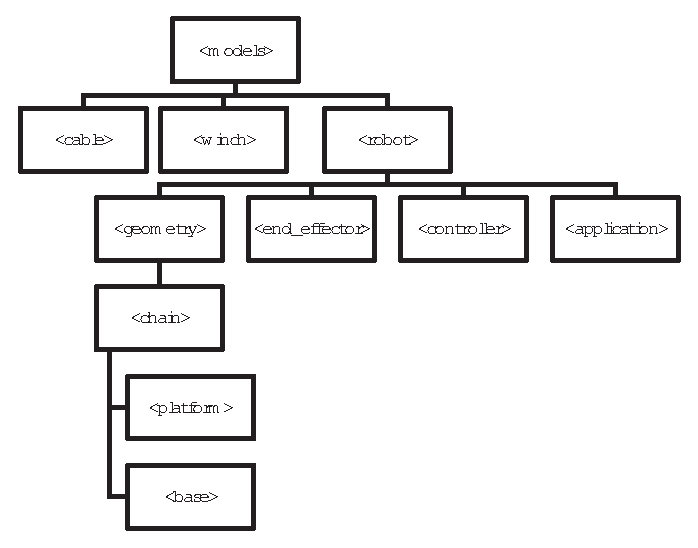
\includegraphics[width=0.8\textwidth]{XmlFileFormatStructure.eps}
  \caption{Logical structure of the XML file format}
  \label{fig:XmlFileFormatStructure}
\end{figure}
It is conceivable that XML files which only contain cable or winch information
within the \<models> tag facilitate data-exchange of these components. These
can be considered as databases of their respective kind. The contents of the
\<models> tag for a specific cable robot using one type of winch and cable
would then be as such:
\begin{verbatim}
<models>
  <robot name="IPAnema2" id="1">
    <!-- properties of the robot will be here -->
  </robot>
  <winch name="Winde1" id="1">
    <!-- properties of the winch will be here -->
  </winch>
  <cable name="SteelCable1" id="1">
    <!-- properties of the cable will be here -->
  </cable>
</models>
\end{verbatim}

The \<models> tag encompasses all the relevant data placed in the tags
\<cable>, \<winch> and \<robot> and has the following attributes:

\begin{table}
  \centering
  \caption{\<models> tag attributes}
  \label{tab:XmlModelTag}
  \begin{tabular}{p{0.3\textwidth}p{0.18\textwidth}p{0.4\textwidth}}
    \hline\hline
    Attribute & Type & Description \\
    \hline
    version & String & Version number of XML schema.\\
    \hline\hline
  \end{tabular}
\end{table}

The relevant parameters for each robot will be placed in the \<robot> tag. The
\<robot> tag contains the attributes outlined in Table~\ref{tab:XmlRobotTag}.
The attributes in the \<robot> tag hold meta-information identifying specific
robot configurations.

\begin{table}
  \centering
  \caption{\<robot> tag attributes }
  \label{tab:XmlRobotTag}
  \begin{tabular}{p{0.3\textwidth}p{0.18\textwidth}p{0.4\textwidth}}
    \hline\hline
    Attribute  & Type  &  Description \\
    \hline
    name & String & Name of the robot / robot design.\\
    id & Int & Unique identifier for this robot.\\
    \[author] & String & Name of the Author or
    Institution responsible for this robot design.\\
    \[generator] & String & Reference to the software tool used to generate this robot.\\
    \[description] & String & Description of the robot design.\\
    \[motion\_pattern] & String (enum) & Type of motion\_pattern this
    robot is able to generate. This indicates the number of
    translational (T) and rotational (R) degrees of freedom, e.g.: 3R3T
    has six d.o.f in Cartesian space. Permitted values are 1T, 2T, 3T,
    1R2T, 2R3T and 3R3T.\\
    \hline\hline
  \end{tabular}
\end{table}

The relevant parameters for each cable will be placed in the \<cable> tag. This
tag does not contain any further sub-tags as the total information relevant to
individual cables is considered relatively small. As such meta-information and
cable parameters are both described within the attributes of the \<cable> tag
presented in section~\ref{sec:XmlCable} cable parameters.

The relevant parameters for each winch will be placed in the \<winch> tag. The
\<winch> tag contains the attributes outlined in Table~\ref{tab:XmlWinchTag}.
The attributes in the \<winch> tag hold meta-information identifying specific
robot configurations.

\begin{table}
  \centering
  \caption{\<winch> tag attributes }
  \label{tab:XmlWinchTag}
  \begin{tabular}{p{0.3\textwidth}p{0.18\textwidth}p{0.4\textwidth}}
    \hline\hline
    Attribute  & Type & Description \\
    \hline
    Name & String & Name of that particular winch type.\\
    Id & Int & Unique identifier for winch type.\\
    \[creator] & String & Name of the creator or institution responsible
    for this robot design.\\
    \[description] & String & Description of winch type.\\
    \hline\hline
  \end{tabular}
\end{table}

\subsection{Cable Parameters}\label{sec:XmlCable}%
Unlike the robot parameters, cable parameters are not considered unique for a
single application. Hence cable types are defined separately in within the
cable tag. These types can be grouped to provide a library of cables which can
be part of a specific robot, or an independent database with only cable types.
The \<cable> tag contains the attributes outlined in
Tab.~\ref{tab:XmlCableTag}. The attributes in the \<cable> tag hold
meta-information identifying cable types and specific cable parameters.

\begin{table}
  \centering
  \caption{\<cable> tag attributes}
  \label{tab:XmlCableTag}
  \begin{tabular}{p{0.3\textwidth}p{0.18\textwidth}p{0.4\textwidth}}
    \hline\hline
    Attribute  & Type  &  Description \\
    \hline
    name & String & Name of that particular cable.\\
    id & Int & Unique identifier for cable type.\\
    \[radius] & Scalar & Radius of the cable \[m].\\
    \[weight] & Scalar & Specific weight of the cable \[kg/m].\\
    \[damping] & Scalar & Specific damping\\
    \[elasticity]& Scalar & Specific elasticity of the cable \[1/N].\\
    \[breaking\_load]& Scalar & Breaking load in \[N]\\
    \[minimum\_load] & Scalar & Minimum load in \[N]\\
    \[max\_length] & Scalar & Maximum cable length in \[m]\\
    \hline\hline
  \end{tabular}
\end{table}

\subsection{Winch}%
Winches are complex assemblies with many different possible layouts. The focus
in this tag will be on parameters directly affecting the cable robot. Similarly
to the cable parameters the winch parameters are combined to only contain
information of specific winches, so that they can be grouped as a database, or
applied to several robot geometries.

Winch parameters are described in the \<winch> tag. Due to the complexity the
physical parameters are grouped in relevant sub-tags within the \<winch> tag.

\begin{table}
  \centering
  \caption{Tags contained within the \<winch> tag}
  \label{tab:XmlWinchTagOverview}
  \begin{tabular}{p{0.3\textwidth}p{0.18\textwidth}p{0.4\textwidth}}
    \hline\hline
    Tag  & Attributes  &  Description \\
    \hline
    \<cable> & In Tab.~\ref{tab:XmlCableTag2} & Relevant winch parameters in relation to the cables.\\
    \<motor> & In Tab.~\ref{tab:XmlMotorTag} & Parameters of the motor drive.\\
    \<drum> & In Tab.~\ref{tab:XmlDrumTag} & Parameters of the cable drum.\\
    \<guiding\_limit> & In Tab.~\ref{tab:XmlGuidinglimitTag} & Description of the possible cable direction vectors from the point of exit\\
    \<linear\_drive> & In Tab.~\ref{tab:XmlLineardriveTag} & Parameters of a linear drive (if used)\\
    \<anchoring> & In Tab.~\ref{tab:XmlAnchoringTag} & Physical description of the anchoring mechanisms (for evaluating attachment to frame)\\
    \hline\hline
  \end{tabular}
\end{table}

Each tag defined in Table~\ref{tab:XmlWinchTagOverview} contains further
attributes to include winch parameters. These attributes listed in the
following tables.

The \<cable> tag contains the attributes listed in Tab.~\ref{tab:XmlCableTag2}.
These attributes contain specific winch parameters relating to the cable
actuated by the winch.

\begin{table}
  \centering
  \caption{\<cable> tag attributes}
  \label{tab:XmlCableTag2}
  \begin{tabular}{p{0.3\textwidth}p{0.18\textwidth}p{0.4\textwidth}}
    \hline\hline
    Attribute & Type & Description \\
    \hline
    nr\_cables & Int & Number of cables per winch. \\
    transmission\_ratio & Scalar & The ratio between motor turns and cable length.\footnote{This value is the best estimate, and theoretically could be calculated with enough information on the winch geometry, but as it is deemed essential to cable robot manipulation it is explicitly stated here. It is conceivable that some winches may have a non-inear transmission ratio; but as of yet the XML Schema does not accommodate for this. Should the need exist a separate tag within the \<winch> tag is likely.} \\
    \[f\_max] & Scalar & Maximum tension force exerted on the cable \[N].\\
    \[f\_hold\_max] & Scalar & Maximum holding force \[N].\\
    \[string\_orientation] & String & Nominal direction of the cable in $\Re^3$\\
    \[dl\_max] & Scalar & Maximum cable length variation \[m]\\
    \[l\_min]& Scalar & Minimum cable length \[m].\\
    \[max\_velocity] & Scalar & Maximum cable velocity \[m/s].\\
    \[max\_acceleration] & Scalar & Maximum cable acceleration \[m/s$^2$].\\
    \[max\_jerk] & Scalar& Maximum cable jerk \[m/s$^3$].\\
    \[position\_sensor\_accuracy] & Scalar & Accuracy of the position sensors \[m].\\
    \[force\_sensor\_accuracy]& Scalar & Accuracy of the force sensors \[N].\\
    \[spring\_constant] & Scalar & Spring constant of the winch \[m/N].\\
    \[length\_offset] & Scalar & Length offset for the cable length \[m].\\
    \hline\hline
  \end{tabular}
\end{table}

The \<motor> tag contains the attributes listed in Tab.~\ref{tab:XmlMotorTag}.
These attributes contain specific winch parameters relating to the motor
specifications.

\begin{table}
  \centering
  \caption{\<motor> tag attributes}
  \label{tab:XmlMotorTag}
  \begin{tabular}{p{0.3\textwidth}p{0.18\textwidth}p{0.4\textwidth}}
    \hline\hline
    Attribute & Type  &  Description \\
    \hline
    motor\_type & String & Type of motors (i.e. servo, stepper, etc.)\\
    \[inertia] & Scalar & Motor inertia in \[kg m$^2$]\\
    \[mass] & Scalar & Motor mass in [kg]\\
    \[max\_power]& Scalar & Motor power [W]\\
    \[angular\_velocity] & Scalar & Angular velocity of motor [rads/s]\\
    \[angular\_acceleration] & Scalar & Angular acceleration of motor[rad/s$^2$]\\
    \[gear\_ratio] & Scalar & Gear ratio of the drive train\\
    \hline\hline
  \end{tabular}
\end{table}

The \<drum> tag contains the attributes listed in Table~\ref{tab:XmlDrumTag}.
These attributes contain specific winch parameters relating to the cable drum
of the winch. All drum parameters are optional parameters.
\begin{table}
  \centering
  \caption{\<drum> tag attributes}
  \label{tab:XmlDrumTag}
  \begin{tabular}{p{0.3\textwidth}p{0.18\textwidth}p{0.4\textwidth}}
    \hline\hline
    Attribute & Type  &  Description \\
    \hline
    \[r\_drum]  &  Scalar & Radius of the drum in [m]\\
    \[l\_drum]  &  Scalar & Length of the drum in [m]\\
    \[nr\_groove] &Scalar & Number of turns of the cable groove on the drum\\
    \[groove\_depth] & Scalar & Groove depth in [m]\\
    \[dfriction]& Scalar & Dynamic friction of drum on mount [N]\\
    \[sfriction]& Scalar & Static friction of drum on mount [N]\\
    \[backlash] & Scalar & Backlash [m]\\
    \hline\hline
  \end{tabular}
\end{table}

The \<guidinglimit> tag contains the attributes listed in
Tab.~\ref{tab:XmlGuidinglimitTag}. These attributes describe the possible cable
feed directions of the winch geometry.

\begin{table}
  \centering
  \caption{\<guidinglimit> tag attributes}
  \label{tab:XmlGuidinglimitTag}
  \begin{tabular}{p{0.3\textwidth}p{0.18\textwidth}p{0.4\textwidth}}
    \hline\hline
    Attribute & Type & Description \\
    \hline
    \[aperture] & Scalar & Angle of the aperture of to define a cone of possible cable orientations in [rad]\\
    \[cone\_offset] & Position Vector & Apex point offset from point $A_i$.\\
    \hline\hline
  \end{tabular}
\end{table}

The \<lineardrive> tag contains the attributes listed in
Tab~\ref{tab:XmlLineardriveTag}. These attributes describe cable winch if a
drum is replaced by a linear drive.

\begin{table}
  \centering
  \caption{\<lineardrive> tag attributes}
  \label{tab:XmlLineardriveTag}
  \begin{tabular}{p{0.3\textwidth}p{0.18\textwidth}p{0.4\textwidth}}
    \hline\hline
    Attribute & Type & Description \\
    \hline
    \[nr\_pulleys] & Int & Number of pulleys\\
    \[min\_length] & Scalar & Minimal length \[m]\\
    \[max\_length] & Scalar & Maximum length \[m]\\
    \[inertia\_moment] & Scalar & Moment of intertia of the entire assembly \[kg\ m$^2$]\\
    \[dfriction] & Scalar & Dynamic friction \[N]\\
    \[sfriction] & Scalar & Satic friction \[N]\\
    \hline\hline
  \end{tabular}
\end{table}

The \<anchoring> tag contains the attributes listed in
Tab.~\ref{tab:XmlAnchoringTag}. These attributes describe cable winch if a drum
is replaced by a linear drive

\begin{table}
  \centering
  \caption{\<anchoring> tag attributes}
  \label{tab:XmlAnchoringTag}
  \begin{tabular}{p{0.3\textwidth}p{0.18\textwidth}p{0.4\textwidth}}
    \hline\hline
    Attribute & Type & Description \\
    \hline
    \[type] & String & A description of the type of anchoring\\
    \[max\_force] & Scalar & Maximum force permitted for this anchoring \[N]\\
    \[acting\_moment] & Position Vector & Vector defining the moment exerted by the winch in \[m]\\
    \hline\hline
  \end{tabular}
\end{table}

\subsection{Geometry and Layout}%
Layout and geometry of the cable robot are described in the \<geometry> tag.
This describes the physical layout which is unique to each robot even for exact
copies of functionality and parts will always contain positioning errors which
can be reflected here. For every winch-platform pair (or cable connection to
the platform) one \<chain> tag is added. This chain describes the geometrical
positions of these kinematic links and mostly governs the robots properties.
The number of cables is represented by the number of \<chain> tags within the
\<geometry> tag. Each chain has its own identification number in order to pair
the right winch and cable types to one specific chain. The \<chain> tag
contains the attributes outlined in Tab.~\ref{tab:XmlChainTag}. The attributes
in the \<chain> tag hold meta-information identifying a chain and pairing the
correct cable/winch type.
%
\begin{table}
  \centering
  \caption{\<chain> tag attributes}
  \label{tab:XmlChainTag}
  \begin{tabular}{p{0.3\textwidth}p{0.18\textwidth}p{0.4\textwidth}}
    \hline\hline
    Attribute & Type & Description \\
    \hline
    id & Int & Unique identifier for this chain beginning with 1\\
    \[winch\_type] & String & Identification of a specific winch which is defined using a \<winch> tag.\\
    \[cable\_type] & String & Identification of a specific cable which is defined using a \<cable> tag.\\
    \hline\hline
  \end{tabular}
\end{table}

The geometric parameters are defined through the tags described in
Tab.~\ref{tab:XmlChainSubTag}.

\begin{table}
  \centering
  \caption{Tags within the \<chain> tag}
  \label{tab:XmlChainSubTag}
  \begin{tabular}{p{0.3\textwidth}p{0.18\textwidth}p{0.4\textwidth}}
    \hline\hline
    Tag & Attribute & Description \\
    \hline
    \<base> & Position Vector & Vector identifying the characteristic exit point of the cable defined in the world coordinate system $\mathcal K_0$. (In the case of a winch with pulley kinematics this would be point $A_i$) in [m]\\
    \<base> & Rotation Matrix or Quaternion or Axis Angle & Winch orientation: When using pulley kinematics the direction of the rotation axis and the reference plane for the determination of the angles.\\
    \<base> & Radius="Scalar" & Radius of the Pulley in [m];\\
    \<platform> & Position Vector & Vector identifying the characteristic end point of the cable on the platform. Defined in the coordinate system of the platform ($\mathcal K_p$)\\
    \<platform> & Rotation Matrix or Quaternion or Axis Angle & Orientation of the coordinate system $\mathcal K_{Bi}$ which describes the characteristics of the cable end point. Defines a normal cable direction.\\
    \hline\hline
  \end{tabular}
\end{table}

A typical robot geometry can be defined as follows:
\begin{verbatim}
<models>
  <robot name="IPAnema2">
    <geometry>
      <!-- A Simple Winch-->
      <chain id=1>
        <base x="1.0" y="2.0" z="0.0"/>
        <platform x="0.1" y="0.05" z="0.0"/>
      </chain>
      <!-- A Winch with orientation -->
      <chain id=2>
        <base x="-1.0" y="2.0" z="0.0" q0="1" q1="0" q2="0" q3="0"/>
        <platform x="-0.1" y="0.05" z="0.0"/>
      </chain>
      <!-- More chain tags follow to describe further connections -->
    </geometry>
  </robot>
  <!-- More robots,  winches, or cable parameters can be placed here -->
</models>
\end{verbatim}
The example defines a cable robot named "IPAnema2" with two winches which is of
cause of little practical use. The first winch is place at $a_1=[1.0, 2.0
,0.0]^T$ and the cable is connected to the mobile platform at $b_1=[0.1,
0.05, 0.0]^T$. The reference coordinate system for the winches is not rotated
with respect to the world coordinate frame since the respective attributes in
the \<base> and \<platform> tags is left out and the default values apply. For
the second winch ($a_2=[-1.0, 2.0, 0.0]^T, b_2=[-0.1, 0.05,
0.0]^T$) an orientation is described for the winches. Here the quaternion
$Q=[1,0,0,0]$ is used to the orientation of the winch.

\subsection{Mobile Platform}%
The \<end\_effector> tag is used to describe the attributes of the mobile
platform. It is to be placed in the \<robot> tag. The \<end\_effector> tag
contains the tags and attributes described in Tab.\ref{tab:XmlEndeffectorTag}.
The attributes in the \<end\_effector> tag holds meta-information of the
platform and specific physical parameters. The geometric information for the
platform's anchor points are stored in the \<chain> tag.

\begin{table}
  \centering
  \caption{Tags within the \<end\_effector> tag}
  \label{tab:XmlEndeffectorTag}
  \begin{tabular}{p{0.3\textwidth}p{0.18\textwidth}p{0.4\textwidth}}
    \hline\hline
    Attribute & Type  &  Description \\
    \hline
    \<end\_effector> & name=\-"String" & Name of the platform\\
    \<end\_effector> & description=\-"String" & Description of platform\\
    \<end\_effector> & mass=\-"double" & Mass in \[kg]\\
    \<end\_effector> & swing\_angle=\-"double" & Permitted cable swing angle \[rad]\\
    \<inertia> & Moment of Inertia Tensor & Platform moment of inertia tensor \[kg\ m$^2$]\\
    \<centre\_of\_gravity> & Position Vector & Center of gravity of the platform define in the platform coordinate system ($\mathcal K_p$) [m$^3$]\\
    \hline\hline
  \end{tabular}
\end{table}

Within the \<end\_effector> tag there are the attributes "name", "description",
"mass", and "swing\_angle", in addition to two tags \<inertia> and
\<centre\_of\_gravity>  which contain more complex data structures inertia
tensor and position vector.

\subsection{Controller}%
The \<controller> tag is used to describe the attributes of the control loop of
the cable robot. It is to be placed in the \<robot> -tag. The \<controller>-tag
contains the attributes described in Tab.~\ref{tab:XmlController}. The
attributes in the \<controller> tag holds meta-information of the controller
and specific physical parameters.

\begin{table}
  \centering
  \caption{\<controller> tag attributes}
  \label{tab:XmlController}
  \begin{tabular}{p{0.3\textwidth}p{0.18\textwidth}p{0.4\textwidth}}
    \hline\hline
    Attribute & Type & Description \\
    \hline
    ipo\_clock & Scalar & interpolator cycle time \[s]\\
    dim\_x & Int & Dimensions of controller variables\\
    delay\_time & Scalar & Time Constant of the delay time in \[s]\\
    time\_discrete & Bool & Indicator whether the control is in discrete time steps "1" or continuous "0".\\
    \hline\hline
  \end{tabular}
\end{table}

The number of inputs and outputs for the controller is defined (similar to with
the \<chain> tag) through the number of tags and is not explicitly stated.
Attributes of the tags  \<input\_port> and \<output\_port> are described in
Tab.~\ref{tab:XmlInputTag} and Tab.~\ref{tab:XmlOutputTag} respectively. The
attributes in of these tags hold meta-information of the input/output.

\begin{table}
  \centering
  \caption{\<input\_port> tag attributes}
  \label{tab:XmlInputTag}
  \begin{tabular}{p{0.3\textwidth}p{0.18\textwidth}p{0.4\textwidth}}
    \hline\hline
    Attribute & Type & Description \\
    \hline
    type & String & Type of input; "enumerated" string with the following values:
    \{lin\_position, rot\_position, lin\_velocity, rot\_velocity, lin\_acceleration, rot\_acceleration, force, torque\}\\
    chain\_id & Int & Identifier of the relevant chain id\\
    \hline\hline
  \end{tabular}
\end{table}


The \<output\_port>-tag and the \<input\_port>-tag, have the same structure.

\begin{table}
  \centering
  \caption{\<output\_port> tag attributes}
  \label{tab:XmlInputTag}
  \begin{tabular}{p{0.3\textwidth}p{0.18\textwidth}p{0.4\textwidth}}
    \hline\hline
    Attribute & Type & Description \\
    \hline
    type & String & Type of output; "enumerated" string with the following values:
    \{lin\_position, rot\_position, lin\_velocity, rot\_velocity, lin\_acceleration, rot\_acceleration, force, torque\}\\
    chain\_id & Int & Identifier of the relevant chain id\\
    \hline\hline
  \end{tabular}
\end{table}

\subsection{Application}
The \<application> tag is used to describe the attributes of the control loop
of the cable robot. It is to be placed in the \<robot> tag. The
\<application>-tag contains the attributes described in
Tab.~\ref{tab:XmlApplicationTag}. The attributes in the \<application> tag
holds meta-information of the specific application for which the cable robot is
design and physical parameters.

\begin{table}
  \centering
  \caption{\<application> tag attributes}
  \label{tab:XmlApplicationTag}
  \begin{tabular}{p{0.3\textwidth}p{0.18\textwidth}p{0.4\textwidth}}
    \hline\hline
    Attribute & Type & Description \\
    \hline
    name & String & Name of the application\\
    \[description] & String & Further description of the application\\
    \[load\_mass] & Scalar & max. mass acting on the platform \[N]\\
    \[load\_moment] & Scalar & max. moment acting on the platform \[Nm]\\
    \[min\_cable\_load] & Scalar & min. acceptable cable load \[N]\\
    \[max\_cable\_load] & Scalar & max. acceptable cable load \[N]\\
    \hline\hline
  \end{tabular}
\end{table}


\chapter{Literature}
The following books are advised as basics for software development:
\begin{itemize}
\item Erich Gamma, Richard Helm, Ralph E. Johnson: \emph{Design Patterns.
    Elements of Reusable Object-Oriented Software}. Prentice Hall 1994.

\item Bjarne Stroustrup: \emph{The C++ Programming Language: Special
    Edition}
    (4th Ed.). Addison Wesley 2000.
\end{itemize}
The following book is helpful to get into the development of Windows GUI using
the Microsoft Foundation Classes (MFC) and the document-view architecture.
\begin{itemize}
\item David J. Kruglinski, George Sheperd, Scot Wingo: \emph{Inside Visual
    C++ 6.0}. MicrosoftPress, 1998.
\end{itemize}
To understand openGL it is worthwhile to study \emph{The red book}:
\begin{itemize}
\item Dave Shreiner, Graham Sellers, John M. Kessenich, Bill M. Licea-Kane:
    \emph{OpenGL Programming Guide: The Official Guide to Learning OpenGL,
    Version 4.3 (8th Edition)}. Addison-Wesley, 2013.
\end{itemize}

Although this documentation focuses on the software part, some fundamental
issues about (cable-driven) parallel robot are essential to understand how
WireLib and WireCenter work. The reference book by Merlet \cite{Merlet2006} is
worthwhile reading to get into parallel robots and lately \cite{Pott2018}
provides a basis for all aspects of cable robot questions.

\begin{thebibliography}{10}
\bibitem{Bouchard2010} Bouchard, S., Moore, B., Gosselin, C.: {O}n the
    ability of a cable-driven robot to generate a prescribed set of wrenches.
\newblock Journal of Mechanisms and Robotics \textbf{2}(1), pp. 1--10 (2010)

\bibitem{Hassan2007} Hassan, M., Khajepour, A.: {M}inimum-norm {S}olution for
    the {A}ctuator
  {F}orces in {C}able-based {P}arallel {M}anipulators based on {C}onvex
  {O}ptimization.
\newblock In: ICRA, pp. 1498--1503 (2007)

\bibitem{Pott2012} Pott, A.: {I}nfluence of {P}ulley {K}inematics on
    {C}able-{D}riven {P}arallel {R}obots.
\newblock In: {L}atest {A}dvances in
  {R}obot {K}inematics, pp. 197--204. Springer (2012)

\bibitem{Pott2009} Pott, A., Bruckmann, T., Mikelsons, L.: {C}losed-form
    {F}orce {D}istribution for {P}arallel {W}ire {R}obots.
\newblock In: {C}omputational {K}inematics, 25--34. Springer (2009)

\bibitem{Verhoeven2004} Verhoeven, R.: {A}nalysis of the {W}orkspace of
    {T}endon-based {S}tewart {P}latforms.
\newblock Ph.D. thesis, {University of Duisburg-Essen}, Duisburg (2004)

\bibitem{Pott2013} Andreas Pott.
\newblock {A}n improved {F}orce {D}istribution {A}lgorithm for
  {O}ver-{C}onstrained {C}able-{D}riven {P}arallel {R}obots.
\newblock In {Frederico Thomas} and {Alba P{\'e}rez Gracia}, editors, {\em
  {C}omputational {K}inematics 2013}.

\bibitem{Pott2018} Andreas Pott.
\newblock {\em Cable-driven Parallel Robots: Theory and Application.}
\newblock Springer, Berlin, 2018.

\bibitem{Merlet2006} Jean-Pierre Merlet.
\newblock {\em {P}arallel {R}obots, 2nd {E}d}.
\newblock Springer-Verlag, 2006.

\bibitem{Perreault2010} Simon Perrault, Philippe Cardou, Cl{\'e}ment Gosselin,
    and Martin J.-D. Otis.
\newblock {G}eometric determination of the interference-free
  constant-orientation workspace of parallel cable-driven mechanisms.
\newblock {\em ASME Journal of Mechanisms and Robotics}, 2(3), 2010.

\end{thebibliography}

\end{document}
% ----------------------------------------------------------------
